%# -*- coding: utf-8-unix -*-
%%==================================================
%% thesis.tex
%%==================================================

% 双面打印
\documentclass[bachelor, openright, twoside, english]{sjtuthesis}
% \documentclass[bachelor, openany, oneside, submit]{sjtuthesis}
% \documentclass[master, review]{sjtuthesis}
% \documentclass[%
%   bachelor|master|doctor|coursepaper, % 必选项,分别是学士,硕士,博士学位论文以及课程论文
%   fontset=fandol|windows|mac|ubuntu|adobe|founder, % 字体选项
%   oneside|twoside,        % 单面打印,双面打印(奇偶页交换页边距,默认)
%   openany|openright,      % 可以在奇数或者偶数页开新章|只在奇数页开新章(默认)
   % english,                % 启用英文模版
%   review,     % 盲审论文,隐去作者姓名、学号、导师姓名、致谢、发表论文和参与的项目
%   submit      % 定稿提交的论文,插入签名扫描版的原创性声明、授权声明
% ]

% 逐个导入参考文献数据库

% \usepackage[
%   separate-uncertainty = true,
%   multi-part-units = repeat
% ]{siunitx} 

\usepackage{hyperref}



\usepackage{url}  %Required
\usepackage{graphicx}  %Required
\usepackage{booktabs}
\usepackage{xspace}
\usepackage{color}
% \usepackage{subfig}
\usepackage{multirow}% http://ctan.org/pkg/multirow
\usepackage{hhline}% http://ctan.org/pkg/hhline
\usepackage[colorinlistoftodos]{todonotes}
\usepackage{siunitx}
\usepackage{amsfonts,amsthm,amsmath}
\usepackage{enumitem}
% \usepackage[belowskip=-15pt,aboveskip=0pt]{caption}
\usepackage[skip=2pt]{caption} % example skip set to 2pt
%\usepackage[belowskip=0pt,aboveskip=0pt]{caption}

% \setlength{\intextsep}{10pt plus 2pt minus 2pt}
\theoremstyle{definition}

\newtheorem{problem}{Problem}

\newcommand{\nop}[1]{}
\newcommand{\Todo}{{\textbf{\color{red}{todo-}}}}
\newtheorem{definition}{Definition}
% general terms for methods
\newcommand{\deepQLearning}{Deep Q-Learning\xspace}
\newcommand{\deepQNetwork}{Deep Q-Network\xspace}
\newcommand{\dqn}{DQN\xspace}

%notations
\newcommand{\notationFont}{\mathit}
\newcommand{\notationVec}{\mathbf}

\newcommand{\agent}{\notationFont{G}}
\newcommand{\agentVec}{\pmb{G}}
% \newcommand{\environment}{\notationFont{E}}
\newcommand{\environmentVec}{\notationVec{E}}
\newcommand{\user}{\notationFont{u}}
\newcommand{\action}{\notationFont{a}}
\newcommand{\actionVec}{\notationVec{a}}
\newcommand{\staterep}{\notationFont{s}}
\newcommand{\staterepVec}{\notationVec{S}}
\newcommand{\obervationrepVec}{\notationVec{O}}
\newcommand{\reward}{\notationFont{r}}
\newcommand{\rewardTotal}{\notationFont{R}}
\newcommand{\queueLength}{\notationFont{L}}
\newcommand{\numOfVehicles}{\notationFont{N}}
\newcommand{\distriOfVehicles}{\notationFont{D}}
\newcommand{\averageWaitingTime}{\notationFont{W}}
\newcommand{\image}{\notationFont{M}}
\newcommand{\phase}{\notationFont{p}}
\newcommand{\pressure}{\notationFont{P}}
\newcommand{\delay}{\notationFont{V}}
\newcommand{\switch}{\notationFont{C}}
\newcommand{\emergencyStop}{\notationFont{O}}
\newcommand{\numleft}{\notationFont{F}}
\newcommand{\durationleft}{\notationFont{D^F}}
\newcommand{\setOfVehicle}{\notationFont{J}}
\newcommand{\setOfLane}{\notationFont{I}}
\newcommand{\laneIndex}{\notationFont{i}}
\newcommand{\vehicleIndex}{\notationFont{j}}

\newcommand{\qnetwork}{\notationFont{Q}}
\newcommand{\expNotation}{\textsl}
\newcommand{\WE}{\expNotation{WE}\xspace}
\newcommand{\EW}{\expNotation{EW}\xspace}
\newcommand{\NS}{\expNotation{NS}\xspace}
\newcommand{\SN}{\expNotation{SN}\xspace}


\newcommand{\WEs}{\expNotation{WE-Straight}\xspace}
\newcommand{\WEl}{\expNotation{WE-Left}\xspace}
\newcommand{\SNs}{\expNotation{SN-Straight}\xspace}
\newcommand{\SNl}{\expNotation{SN-Left}\xspace}


\newcommand{\baselineNotation}{\textsf}
\newcommand{\FT}{\baselineNotation{FixedTime}\xspace}
\newcommand{\SOTL}{\baselineNotation{SOTL}\xspace}
\newcommand{\Greenwave}{\baselineNotation{GreenWave}\xspace}
\newcommand{\Maxpressure}{\baselineNotation{MaxPressure}\xspace}
\newcommand{\GWRL}{\baselineNotation{GWRL}\xspace}
\newcommand{\NIPS}{\baselineNotation{GRL}\xspace}
\newcommand{\Deeplight}{\baselineNotation{IntelliLight}\xspace}
% \newcommand{\PressLight}{\expNotation{PressLight-s}\xspace}
\newcommand{\base}{\baselineNotation{base}\xspace}
\newcommand{\SDeeplight}{\baselineNotation{base+seg}\xspace}
\newcommand{\NDeeplight}{\baselineNotation{base+neigh}\xspace}
\newcommand{\SNDeeplight}{\baselineNotation{base+neigh+seg}\xspace}
\newcommand{\PressLight}{\baselineNotation{PressLight}\xspace}
% \newcommand{\PressLight}{\expNotation{CTRL}\xspace}

\newcommand{\HeavyFlat}{{HeavyFlat}}
\newcommand{\HeavyPeak}{{HeavyPeak}}
\newcommand{\LightFlat}{{LightFlat}}
\newcommand{\LightPeak}{{LightPeak}}

\addbibresource{bib/thesis.bib}
% \addbibresource{bib/chap2.bib}

%# -*- coding: utf-8-unix -*-
% !TEX program = xelatex
% !TEX root = ../thesis.tex
% !TEX encoding = UTF-8 Unicode
%TC:ignore
\title{面向多路口交通信号灯控制的深度强化学习算法}
\author{陈诧姹}
\advisor{张伟楠}
% \coadvisor{某某教授}
\defenddate{2019年6月10日}
\coursename{某某课程}
\school{上海交通大学}
\institute{电子信息与电气工程学院}
\studentnumber{515021910302}
\cnacademicdegree{工学学士}
\major{计算机科学与技术}
\keywords{上海交大, 饮水思源, 爱国荣校}

\englishtitle{Deep reinforcement learning for multi-intersection traffic signal control}
\englishauthor{\textsc{Chacha Chen}}
\englishadvisor{Prof. \textsc{Weinan Zhang}}
% \englishcoadvisor{Prof. \textsc{Uom Uom}}
\englishschool{Shanghai Jiao Tong University}
\englishinstitute{\textsc{Depart of Computer Sience and Engineering, School of Electronic Information and Electrical Engineering} \\
  \textsc{Shanghai Jiao Tong University} \\
  \textsc{Shanghai, P.R.China}}
\englishinstitutemaster{Depart of Computer Sience and Engineering, \\ School of Electronic Information and Electrical Engineering}
\englishmajor{A Very Important Major}
\englishdate{Dec. 17th, 2014}
\enacademicdegree{Bachelor of Engineering}
\englishstudentid{515021910302}
\englishkeywords{SJTU, bachelor thesis, XeTeX/LaTeX template}
%TC:endignore
  % NOTE: the enclosed commands must be executed in preamble

\begin{document}

% 无编号内容:中英文论文封面、授权页
\maketitle
\makeatletter

\ifsjtu@coursepaper
% 摘要 部分课程论文需要,可以自行选择添加或者去除
% %# -*- coding: utf-8-unix -*-
% !TEX program = xelatex
% !TEX root = ../thesis.tex
% !TEX encoding = UTF-8 Unicode
%%==================================================
%% abstract.tex for SJTU Master Thesis
%%==================================================

\begin{abstract}


\end{abstract}

\begin{englishabstract}


\end{englishabstract}



% 目录 部分课程论文需要,可以自行选择添加或者去除
% \tableofcontents

\else
  \ifsjtu@submit\relax
    \includepdf{pdf/original.pdf}
    \cleardoublepage
    \includepdf{pdf/authorization.pdf}
    \cleardoublepage
  \else
    \ifsjtu@review\relax
    % exclude the original claim and authorization
    \else
      \makeDeclareOriginal
      \makeDeclareAuthorization
    \fi
  \fi
  \frontmatter % 使用罗马数字对前言编号

  % 摘要
  %# -*- coding: utf-8-unix -*-
% !TEX program = xelatex
% !TEX root = ../thesis.tex
% !TEX encoding = UTF-8 Unicode
%%==================================================
%% abstract.tex for SJTU Master Thesis
%%==================================================

\begin{abstract}


\end{abstract}

\begin{englishabstract}


\end{englishabstract}



  % 目录、插图目录、表格目录
  \tableofcontents
  \listoffigures
  \addcontentsline{toc}{chapter}{\listfigurename}     % 将插图目录加入全文目录
  \listoftables
  \addcontentsline{toc}{chapter}{\listtablename}      % 将表格目录加入全文目录
  \listofalgorithms
  \addcontentsline{toc}{chapter}{\listalgorithmname}  % 将算法目录加入全文目录

  \include{tex/symbol} % 主要符号、缩略词对照表
\fi

\makeatother
\mainmatter % 使用阿拉伯数字对正文编号

% 正文内容
% introduction.tex

\section{Introduction}
\label{sec:introduction}
Traffic congestion is a growing problem that continues to plague urban areas with negative outcomes to both the traveling public and society as a whole. These negative outcomes will only grow over time as more people flock to urban areas. In 2014, traffic congestion costs Americans over \$160 billion in lost productivity and wasted over 3.1 billion gallons of fuel~\cite{Econ14}. Traffic congestion was also attributed to over 56 billion pounds of harmful CO2 emissions in 2011~\cite{schrank20152015}. 
In the European Union, the cost of traffic congestion was equivalent to 1\% of the entire GDP~\cite{schrank2012tti}.
Mitigating congestion would have significant economic, environmental and societal benefits.
Signalized intersections are one of the most prevalent bottleneck types in urban environments, and thus traffic signal control plays a vital role in urban traffic management.

\begin{figure}[t]
\centering
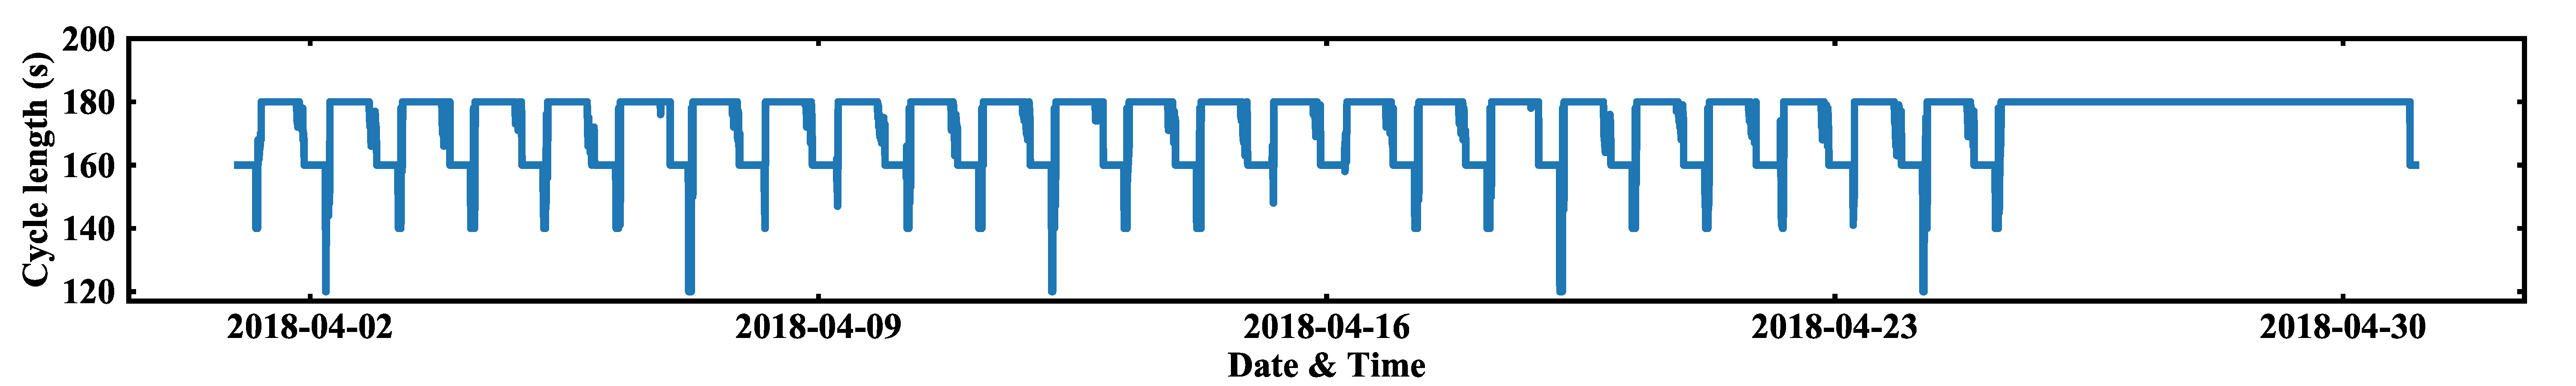
\includegraphics[width=0.99\textwidth]{figures/timing.pdf} 
\caption{Traffic signal timing in a city. The cycle length rarely changes.}
\label{fig:timing}
\end{figure}


\subsection{Current Situation}
In many modern cities today, the widely-used adaptive traffic signal control systems such as SCATS~\cite{SCATS} and SCOOT~\cite{hunt1981scoot,hunt1982scoot} heavily rely on manually designed traffic signal plans. Such manually set traffic signal plans are designed to be dynamically selected according to the traffic volume detected by loop sensors. However, many intersections do not have loop sensors installed or the loop sensors are poorly maintained. Moreover, the loop sensors are activated only when vehicles pass through them, thus they can only provide partial information about the vehicle through them. As a result, the signal cannot perceive and react to the real-time traffic patterns, and engineers need to manually change the traffic signal timings in the signal control system under certain traffic condition scenarios. Figure~\ref{fig:timing} shows the traffic signal timing at an intersection in a city of China and the traffic signal timing rarely changes regardless of the real traffic changes throughout the day.


\subsection{Opportunities}
\emph{First, today we have much richer information that can be collected from various sources.} Traditional traffic signal control relies on data from loop sensors, which can only sense the vehicle passing. However, new data sources are quickly becoming available that can serve as input for traffic signal control purposes. For instance, street-facing surveillance cameras used for security purposes can also provide a more detailed depiction of  the traffic situation on nearby roads -- specifically, how many cars are waiting in the lane, how many cars are taking turns, where they are located, and how fast they are traveling. In addition, large-scale trajectory data can be collected from various sources such as navigation applications (e.g., Google Maps),  ride-sharing platforms (e.g., Uber) and GPS-equipped vehicles that share information with the nearby infrastructure (e.g., connected vehicles). Such data provide us with more insight about how vehicles arrive to intersections. We have reached a stage of abundant mobility information that can describe the traffic dynamics in the city more clearly, which is an essential resource for us to improve the traffic control system.


 
\begin{figure}[htbp]
\centering
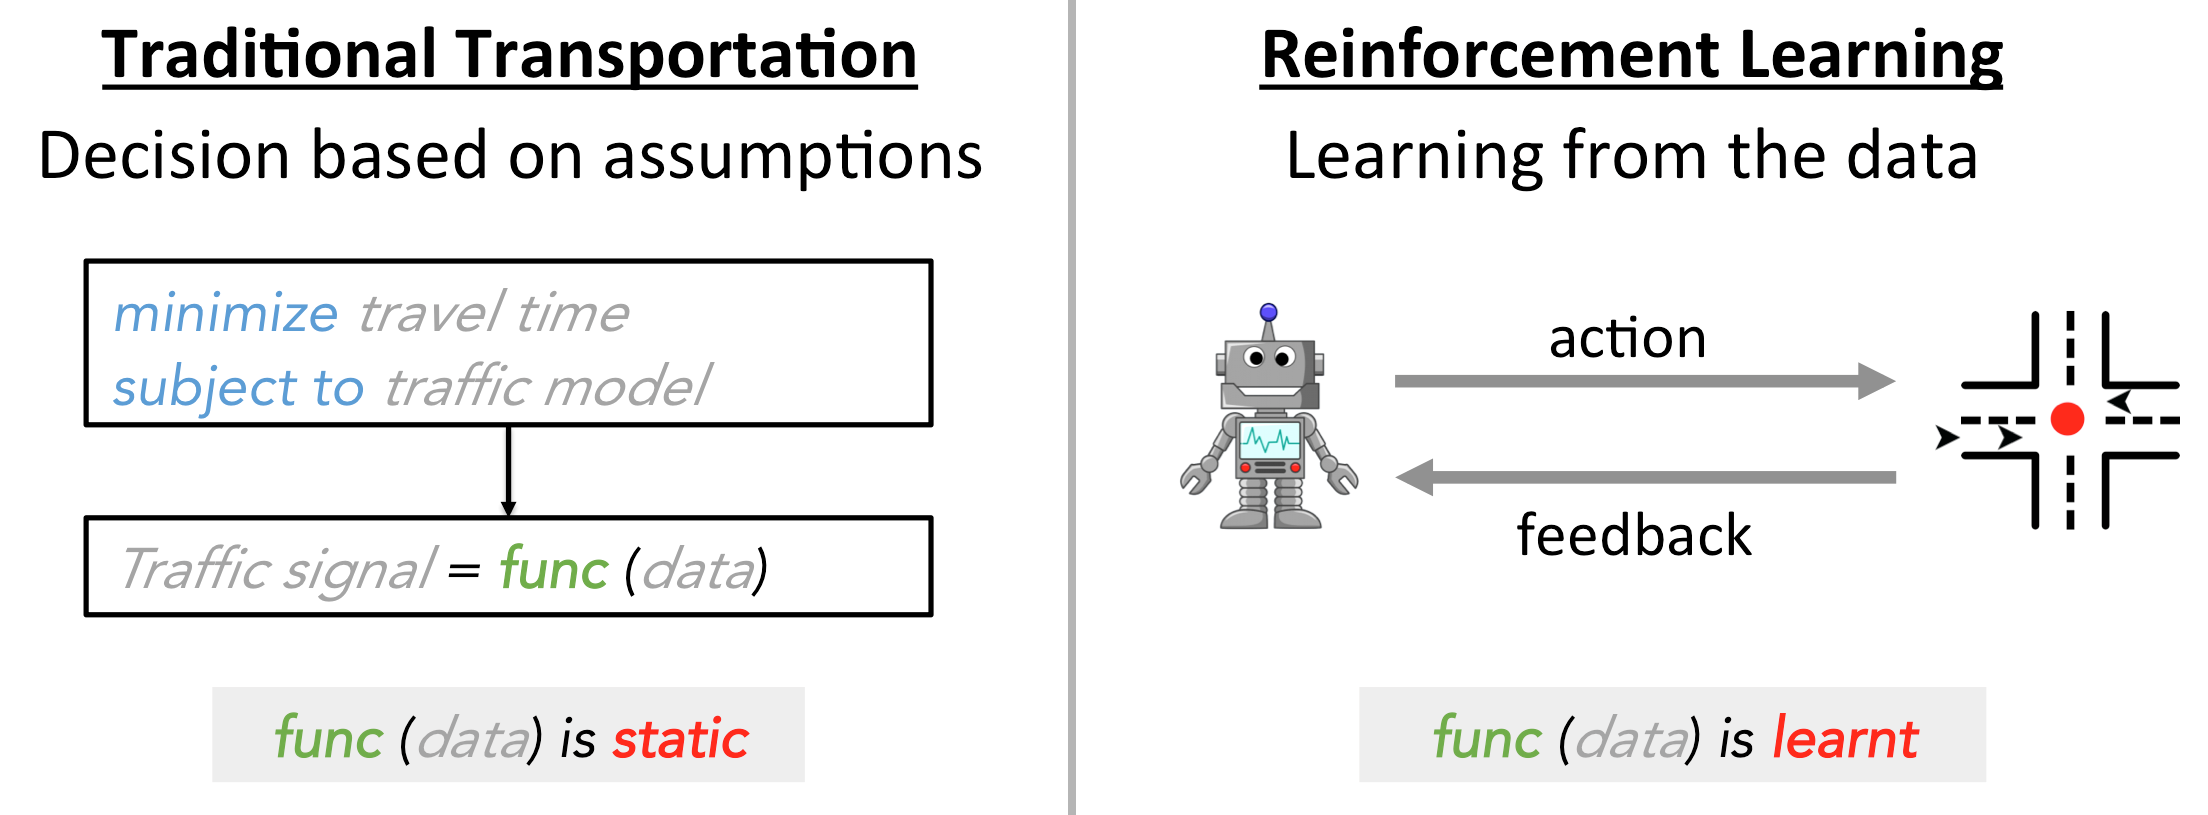
\includegraphics[width=0.7\columnwidth]{fig/optimizationvsRL.png}
\caption{Difference between traditional transportation approach and machine learning approach.}
\label{fig:optvsrl}
\end{figure}

\emph{Second, today we have much stronger computing power and advanced computational models.} The typical approach that transportation researchers take is to cast traffic signal control as an optimization problem under certain assumptions about the traffic model, e.g., vehicles come in a uniform and constant rate~\cite{RPM04}.  Various (and sometimes strong) assumptions have to be made in order to make the optimization problem tractable. The key issue here is that these assumptions deviate from the real world and often do so significantly. As we know, real-world traffic condition evolves in a complicated way, affected by many factors such as driver's preference, interactions with vulnerable road users (e.g. pedestrians, cyclists, etc.), weather and road conditions, just to name a few. These factors can hardly be fully described in a traffic model.


On the other hand, machine learning techniques can directly learn from the observed data without making unrealistic assumptions about the model. However, typical supervised learning does not apply here because existing traffic signal control systems follow pre-defined signal plans so we do not have enough training data to differentiate good and bad traffic signal plan strategies. Instead, we have to first take actions to change the signal plans and then learn from the outcomes. This trial-and-error approach is also the core idea of reinforcement learning (RL). In essence, an RL system generates and executes different strategies (e.g., for traffic signal control) based on the current environment. It will then learn and adjust the strategies based on the feedback from the environment. This reveals the biggest difference between transportation approaches and our RL approaches, which is illustrated in Figure~\ref{fig:optvsrl}: in traditional transportation research, the model $func(data)$ is static; in reinforcement learning, the model is dynamically learned through trial-and-error in the real environment.





% !TEX root = main.tex
% \chapter{Introduction}
% \label{chap:intro}

\chapter{Related Work}
\label{chap:related}
\textbf{Individual Traffic Signal Control.}
Individual traffic signal control has been investigated extensively in the field of transportation. These methods try to optimize the travel time or delay of vehicles~\cite{Gart83,Henr84,Boil06,SeHe97,Liang18}, building on the assumption that vehicles are arriving and moving in a specific pattern. Recently, reinforcement learning based methods attempt to address this problem by directly learning from the data~\cite{Wier00,MaDH16}. Earlier work using tabular Q-learning~\cite{APK03,ElAb10} can only deal with discrete state representations. Recent work using deep Q-learning~\cite{liLW16,VaOl16,wei2018intellilight} and policy gradient~\cite{MSCH17,Casa17PG} can cope with more complex continuous state representation, and hence have shown better performance.

\textbf{Conventional Multi-intersection Traffic Signal Control.}
Conventional multi-intersection control usually requires the intersections to have the same cycle length, coordination can be achieved by setting a fixed offset (i.e., the time interval between the beginnings of green lights) among all intersections~\cite{urbanik2015signal} in grid networks with homogeneous blocks. In fact, it is not an easy task to even provide coordination along an arterial, given traffic of opposite directions usually cannot be facilitated simultaneously. To solve this problem, some optimization-based methods~\cite{robertson1969transyt,little1981maxband} are developed to minimize vehicle travel time and/or the number of stops at multiple intersections. 
Systems like SCATS and SCOOT also have internal selection or optimization processes to modify cycle length, phase splits and offsets ~\cite{kergaye2010comparative}. Instead of optimizing offsets, max-pressure~\cite{MP13,MP13book} aims to maximize throughput of the network so as to minimizing the travel time. However, these approaches still rely on assumptions to simplify the traffic condition, and do not guarantee optimal results in the real world.

\textbf{RL-based Multi-intersection Traffic Signal Control.}
Since recent advances in RL improve the performance on isolated traffic signal control~\cite{VaOl16,wei2018intellilight}, efforts have been made to design strategies that control multiple intersections. \textit{One way} is to consider explicit coordination mechanisms between learning agents using coordination graphs\cite{KWBV08,VaOl16}, extending \cite{Wier00} using max-plus algorithm. Since all the above methods need to negotiate between the agents in the whole network, they are computationally expensive. \textit{Another way} is to use individual RL agents to control the traffic signals in the multi-intersection system~\cite{ElAA13,ALUK10,da2006adaptive}. These methods are more scalable, since each agent makes its own decision based on the information from itself and neighboring intersections without explicit coordination. Our proposed method also follows this direction. However, none of the existing studies draw a connection with traditional transportation methods. 

%they only focus on rewards and overlook the adaptability of the algorithms to the real traffic. Therefore, they cannot interpret why the learned light signal changes corresponding to the traffic. In this paper, we try to test the algorithms in different traffic setting, and add more interpretation other than just reward.

\nop{
Conventional control methods in isolated intersections use closed-form solutions given by optimization of operational parameters based on assumptions and constraints, while reinforcement learning methods have proven useful in this problem as they are able to learn from data collected from sensors in a more intelligent and adaptive way. \Todo-Guanjie, make it shorter


\begin{itemize}
\item Coordinated method
\item non-Coordinated method
\item centralized control(searching space)
\end{itemize}

Isolated traffic signal control has been investigated extensively in the field of transportation. These methods try to optimize the travel time or delay of vehicles~\cite{Gart83,Henr84,Boil06,SeHe97}, building on the assumption that vehicles are arriving and moving in a specific pattern. Recently, reinforcement learning based methods attempt to attack this problem by directly learning from the data~\cite{wiering2000multi,mannion2016experimental}. Earlier work using tabular Q-learning~\cite{APK03,ElAb10} can only deal with discrete state representations. Recent work using deep Q-learning~\cite{li2016traffic,van2016coordinated,wei2018intellilight} and policy gradient~\cite{mousavi_traffic_2017,mousavi_traffic_2017} can cope with more complex continuous state representation, and hence have shown better performance.

However, major challenges lie in the control of multi-intersection scenario, i.e., along an arterial and inside a network. Current methods generally have two categories, centralized methods, and decentralized methods~\cite{SQAS15}. 


Centralized methods are implemented either with pre-defined or with traffic-responsive methods, while both of them are not easy to scale.  Pre-defined centralized approaches usually use historical data to calculate splits and cycle times so as to maximize the flow in a specific direction. One of the widely-used pre-defined centralized coordinated methods in transportation engineering is through "Green Wave", i.e., vehicle will see a progressive cascade of green lights, to optimize the travel time of vehicles along an arterial. The problem with fixed coordination is that the solution is based on an aggregated average traffic pattern, and therefore does not necessarily address real-time situations satisfactorily. Traffic responsive centralized systems, on the other hand, use a centralized agent to control all intersections for the sake of coordination. Each intersection is typically controlled by traffic-responsive methods for changing signal phases. For systems like SCATS or SCOOT, the decisions are made after internal selection and optimization inside the control systems, which may not reflect real-world consequences. \todo{ZY will work on this part}Centralized methods work well only with well-defined traffic volume patterns. In cities where these patterns are not clearly separable (e.g., cities where business centers are no longer located exclusively downtown), coordination may not be effective. What's more, when adding new intersections into the system, centralized methods are not easy to scale, since it may require a large number of central updates of control strategies, or even learning from scratch. 

\nop{Isolated traffic responsive systems, on the other hand, use inductive loop sensors to determine if there is a long queue of stopped cars, but this decision is only locally optimal.
\todo{In both SCATS and SCOOT systems there are coordination between intersections. Maybe say "the decisions are made after internal selection and optimization inside the control systems, which may not reflect real-world consequences"}

In this sense, traffic responsive coordinated control may have a better performance. One type of solution is centralized methods which requires a centralized agent to control all intersections for the sake of coordination. Each intersection is typically controlled by fixed-time plans for changing signal phases, which is largely reply \todo{dependent?} on prior knowledge. For systems like SCATS or SCOOT, the baseline plans of signal settings are predetermined based on engineering experience. This approach works well only in traffic networks with well defined traffic volume patterns\todo{these adaptive methods  do address changes in traffic}. In cities where these patterns are not clearly separable (e.g., cities where business centers are no longer located exclusively downtown), coordination may not be effective. What's more, when adding new intersections into the system, centralized methods are not easy to scale, since it may require a large number of central updates of control strategies, or even learning from scratch. 
}

In this sense, decentralized methods may be more scalable and practicable. Decentralized methods make use of isolated traffic signal control methods, using the information from both target and surrounding intersections. They are computationally less demanding because they only need and maintain relevant information from surrounding intersections/controllers. By plugging new intersection controllers into the system, the decentralized systems are easy to scale. 

However, decentralized methods assume relatively static traffic environments, and are hence far from the real case. What's more, they only focus on rewards and overlook the adaptability of the algorithms
to the real traffic. Therefore, they cannot interpret why the learned light signal changes corresponding to the traffic. In this paper, we try to test the algorithms in different traffic settings and add more interpretations other than reward. As far as we know, it is the first time that the policy learned by the reinforcement learning control agents are interpreted using the traditional transportation coordination method on an arterial.

\nop{Multi-intersection traffic light control has attracted a lot of attention in recent years due to its essential role in adjusting traffic. Current methods generally have two categories, centralized methods, and de-centralized methods. 

Centralized methods use a centralized agent to control all intersections for the sake of cooperation. Each intersection is typically controlled by fixed-time plans for changing signal phases, which is largely reply on prior knowledge. For systems like SCATS or SCOOT, the cooperation rules are defined by human experts (based on ). These rules do not adapt to dynamically changing traffic in real time. 

In general, centralized methods and systems can not scale to large arterials. Traditional centralized systems are usually designed around the larger scale, therefore, adding some controllers requires a large number of central updates of computers and softwares. The operation is relatively complicated and the operator must adjust many parameters. The maintenance of highly skilled and trained operators is expensive.


Decentralized systems rely on the control strategies of individual signal. They are computationally less demanding because they only need and maintain relevant information from surrounding intersections/controllers.

By plugging new controllers into the system, distributed systems are scalable and easy to scale.

The establishment and operation of a decentralized system is often inexpensive because there is no need for a reliable and direct communication network between the central computer and the local controller in the field. As a result, inexpensive communication alternatives such as wireless communication networks have created viable options that significantly reduce system cost}
}

% \input{introduction}
\chapter{Deep Reinforcement Learning for Traffic Signal Control along Arterials}
\label{chap:arterial}
% !TEX root = main.tex

% !TEX root = main.tex
\section{Overview}
\label{sec:intro}
Traffic congestion continues to plague urban environments. Traffic signals serve as one of the most critical bottlenecks that cause congestion, but properly timing signals can often effectively mitigate congestion. Many studies proposed methods to optimize signal timings at isolated intersections. These studies range from manually adjusting signal timings based on expected traffic patterns over some time period~\cite{Mill63}, to actuated signals that adjust signal timings around pre-set values based on current traffic patterns~\cite{CoGD13}, and lastly to adaptive signals that more flexibly adjust signal timings to optimize some objective (usually minimize travel time or queue lengths at the intersection). More recently, reinforcement learning (RL) techniques have been applied to the real-time traffic signal control problem for a single intersection~\cite{VaOl16,wei2018intellilight}; these efforts have shown that RL might provide superior performance over conventional methods. 

However, in urban environments, signals are often in close proximity and this complicates the signal timing problem. Specifically, vehicles departing from one signal influence the arrival pattern of vehicles to the next downstream intersection. Thus, optimizing of signal timings for adjacent traffic signals must be done jointly, which is commonly known as coordinating signal timings. Failure to do so can lead to decisions being made at one signal that can deteriorate traffic operations at another. This is similar to the prisoner's dilemma~\cite{poundstone1993prisoner} in game theory in which locally optimal decisions lead to deterioration of global performance. 

Much effort has been performed to design strategies that explicitly consider coordination between adjacent signals. This includes manually adjust offsets (i.e., time between green signal initiation at adjacent intersections)~\cite{urbanik2015signal}, coordinated graphs for information sharing between intersections~\cite{KWBV08,VaOl16}, or simply using a single, central agent to control all the intersections simultaneously~\cite{brockfeld2001optimizing}. However, explicitly coordinating in this way offers many drawbacks. Current coordinated control requires prior knowledge of traffic patterns and road length to calculate optimal offsets, road structure information to build coordinated graph, etc. The obtained solutions are specifi c to the road network structure. When these features change (e.g., when new intersections are considered), the prevailing coordination policy must be created again. Centralized approaches can alleviate this but these result in large-scale optimization problems that are often not computationally feasible, especially in real-time. Information sharing approaches also rely on large communications networks to share information between signals, and such information is not feasible to obtain. Thus, a central question becomes: \textit{can traffic signal controls operating locally with limited information sharing be able to properly coordinate operations on arterials?}

The chapter proposes a method that implicitly provides coordination through a decentralized RL approach. One of the most emphasized point against implicit-coordination is that control will lead to local optimum without explicit coordination. However, this is only true when traffic signals cannot exchange any information between them, like players engaging in a non-cooperative game. If the information can be shared, even it is between adjacent traffic signals only, it is still possible to achieve promising performance with limited communication.

However, such an attempt is non-trivial with respect to the design of rewards and states in RL. While one of the most important measure in transportation area is the average travel time of all vehicles which is hard to measure instantly, existing studies~\cite{Wier00,VaOl16,wei2018intellilight} take an ad-hoc approach to define reward and state for traffic signal control. Usually they define the reward function as a weighted linear combination of several components, such as queue length, waiting time, number of switches in traffic signal, and sum of delay. Their states include components such as queue length, number of cars, waiting time, and current traffic signal. In recent work~\cite{VaOl16,wei2018intellilight}, images of vehicles' positions on the roads are also considered in the state. 

These ad-hoc design will cause several problems that hinder the application of RL in the real world. First, the engineering details in formulating the reward and state could significantly affect the results. For example, if the reward is defined as a weighted linear combination of several terms, the weights on each terms are tricky to set and the minor difference in weight setting could lead to dramatically different results and policies. Second, the state representation could be in a high-dimensional space, especially when using traffic images as part of the state representation~\cite{VaOl16,wei2018intellilight}. Such a high-dimensional state representation will need much more training data samples to learn and the model may not even converge.

In this chapter, we propose a specific reward and state design that is provably suitable for optimizing the average travel time of all vehicles. Specifically, inspired by a classical transportation method~\cite{MP13}, we use the ``pressure'' as reward and the phase and distribution of vehicles as state. We carefully examine this method under an arterial setting with common signal control strategies that were noted in the transportation field~\cite{newell1981blocking}. Specifically, we compare our method with the optimal coordination strategy obtained from the transportation field, which provides a green wave in which vehicles do not have to stop while traversing the arterial. Under the synthetic data where providing a green wave is the optimal solution, the proposed method can achieve the same performance and automatically form a green wave, which proves our effectiveness in achieving coordination. \textit{This is the first time that a RL method in multi-intersection control is interpreted in connection with traditional methods in transportation area.} In summary, our contributions are as follows:
\begin{itemize}
\item We propose that without explicit coordination strategy, RL method through proper reward and state design can also achieve the effect of coordination along the arterial. 
\item We interpret our RL policy in connection with traditional transportation methods. Our model is tested under a well-designed experiment setting on synthetic data, where there is a closed form optimal solution that has been mathematically justified by transportation theories. To the best of our knowledge, this is the first time that the policy learned by RL is corresponded with the cooperation strategy of traditional transportation methods.
\item Our approach is tested on both synthetic and real-world data and the results show that our method achieves the same optimal performance under simplified settings on synthetic data and outperforms various baseline methods in real-world data.
\end{itemize}

\nop{
\begin{figure}[htbp!]
  \centering
   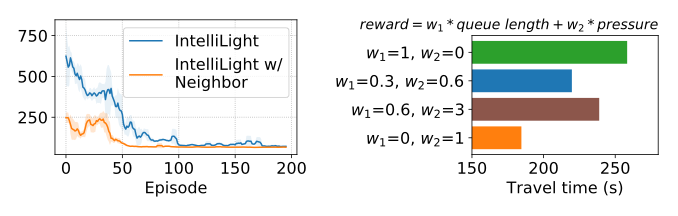
\includegraphics[width=0.48\textwidth]{figures/intro.png}
    \caption{Simultaneous signal setting  determination and coordination}
   \label{fig:intro}
   \vspace{-5mm}
\end{figure}


Conventional coordination consider explicit coordination through analytical optimization under simplified assumption, which cannot be dynamically adjusted to real-time traffic. In recent years, reinforcement learning (RL) techniques have been used on real-time traffic signal control for a single intersection and shown superior performance over conventional methods. Meanwhile, much effort has been performed to design strategies that explicitly coordinate between intersections, such as hand-crafted offsets of phases between intersections, coordinated graphs for information sharing between intersections, or just using one central agent to control all the intersections. However, it is still an open question in the city-wide traffic light control: \textit{to explicitly coordinate, or not?}


Traffic signals are inherently connected:  departures from one intersection directly impact arrival patterns to the next. This leads to strategies that explicitly account for this coordination since adjusting one signal's timings will influence operations at others. Without explicit coordination between individual-level signals, a traffic signal can only optimize based on its own traffic conditions, which can easily lead to deterioration of traffic at other intersections. This is similar to the prisoner's dilemma in game theory. Individual agents move towards optimal solutions locally, but this does not yield a global optimal solution.

However, explicitly accounting for coordination is not computationally efficient. In fact, at the network-wide level, such problems are impossible to formulate and solve in a realistic manner when interactions among a large number of intersection are considered simultaneously. The current coordinated control requires prior knowledge (e.g., have to know traffic pattern and road length to calculate offset, road structure information to build coordinated graph, etc.) and proposes signal control plans for the specified road structure. With new intersections added into the system, the current coordinated control policy may need to be re-organized or re-learned from scratch. Local optimization is more computationally efficient than explicitly coordinated control since it only need to maintain local information.


The chapter stands in the line of non-explicit coordination for the signal control on the arterials. One of the most emphasized points in explicit-coordination is that control will lead to local optimum without explicit coordination. However, this is only true when traffic signals cannot exchange any information between them, like players engaging in a non-cooperative game. If information can be shared between traffic signals, it is still possible to achieve promising performance with limited communication.

However, such an attempt is non-trivial with following questions: a) for an individual intersection, what information of its neighbors needs to be shared to ensure a timely coordination? b) for multiple intersections, how can they learn to optimize the performance of the system as soon as possible to avoid spreading congestions?
To address the first question, in this chapter, we propose to use deep reinforcement learning (DRL) techniques for individual-level control, given the distribution of the vehicle on the approaching and receiving lanes as contextual information from neighboring intersections.
For the second question, learned knowledge from source intersection are transferred to a new one. With each intersection control considered as a subproblem in the larger arterial, we can then re-use the source’s knowledge (e.g., Q-function in RL) for each subproblem in the target, rather than learning from scratch for target intersections.

}


% !TEX root = main.tex

\section{Related Work}
\subsection{Individual traffic signal control.}
Individual traffic signal control has been investigated extensively in the field of transportation. These methods try to optimize the travel time or delay of vehicles~\cite{Gart83,Henr84,Boil06,SeHe97}, building on the assumption that vehicles are arriving and moving in a specific pattern. Recently, reinforcement learning based methods attempt to address this problem by directly learning from the data~\cite{Wier00,MaDH16}. Earlier work using tabular Q-learning~\cite{APK03,ElAb10} can only deal with discrete state representations. Recent work using deep Q-learning~\cite{liLW16,VaOl16,wei2018intellilight} and policy gradient~\cite{MSCH17} can cope with more complex continuous state representation, and hence have shown better performance.

\subsection{Conventional coordinated traffic signal control.}
Conventional coordinated control usually requires the intersections to have the same cycle length, and traffic of selected movements is facilitated through modifying the offset (i.e., the time interval between the beginnings of green lights) between consecutive intersections. In grid networks with homogeneous blocks, like in dense downtown areas, the coordination can be achieved by setting a fixed offset among all intersections~\cite{urbanik2015signal}. However, few networks are so uniform for such simple treatments. In fact, it is not an easy task to even provide coordination along an arterial, given traffic of opposite directions usually cannot be facilitated simultaneously. To solve this problem, some optimization-based methods, such as TRANSYT~\cite{robertson1969transyt} and MAXBAND~\cite{little1981maxband}, are developed to minimize vehicle travel time and/or number of stops at multiple intersections. 
Some traffic control systems such as SCATS and SCOOT also have internal selection or optimization processes to modify cycle length, phase splits and offsets ~\cite{kergaye2010comparative}. However, such approaches still rely on assumptions to simplify the traffic condition, and do not guarantee optimal results in real world.

\subsection{RL-based coordinated traffic signal control.}
Since recent advances in RL  improve the performance on isolated traffic signal control~\cite{VaOl16,wei2018intellilight}, efforts have been performed to design strategies that cooperate multiple RL agents. \cite{KWBV08} and \cite{VaOl16} consider explicit coordination mechanisms between learning agents using coordination graphs, extending \cite{Wier00} using max-plus algorithm. \cite{yang2005intelligent} and~\cite{france2003multiagent} propose to use hierarchical multi-agent RL for global optimization on traffic signal control. Since all the above methods need to negotiate between the agents in the whole network,  they are computationally expensive. 

There are also a line of studies that use individual RL agents to control the traffic signals in the multi-intersection system~\cite{ElAA13,ALUK10,da2006adaptive}. These methods are more scalable, since each agent makes its own decision based on the information from itself and neighboring intersections without explicit coordination. Our proposed method also follows this direction. However, none of existing studies draw a connection with traditional transportation methods. We are the first work to draw such a connection and show that our RL method can automatically learn a green wave policy.

%they only focus on rewards and overlook the adaptability of the algorithms to the real traffic. Therefore, they cannot interpret why the learned light signal changes corresponding to the traffic. In this chapter, we try to test the algorithms in different traffic setting, and add more interpretation other than just reward.

\nop{
Conventional control methods in isolated intersections use closed-form solutions given by optimization of operational parameters based on assumptions and constraints, while reinforcement learning methods have proven useful in this problem as they are able to learn from data collected from sensors in a more intelligent and adaptive way. \Todo-Guanjie, make it shorter


\begin{itemize}
\item Coordinated method
\item non-Coordinated method
\item centralized control(searching space)
\end{itemize}

Isolated traffic signal control has been investigated extensively in the field of transportation. These methods try to optimize the travel time or delay of vehicles~\cite{Gart83,Henr84,Boil06,SeHe97}, building on the assumption that vehicles are arriving and moving in a specific pattern. Recently, reinforcement learning based methods attempt to attack this problem by directly learning from the data~\cite{wiering2000multi,mannion2016experimental}. Earlier work using tabular Q-learning~\cite{APK03,ElAb10} can only deal with discrete state representations. Recent work using deep Q-learning~\cite{li2016traffic,van2016coordinated,wei2018intellilight} and policy gradient~\cite{mousavi_traffic_2017,mousavi_traffic_2017} can cope with more complex continuous state representation, and hence have shown better performance.

However, major challenges lie in the control of multi-intersection scenario, i.e., along an arterial and inside a network. Current methods generally have two categories, centralized methods, and decentralized methods~\cite{SQAS15}. 


Centralized methods are implemented either with pre-defined or with traffic-responsive methods, while both of them are not easy to scale.  Pre-defined centralized approaches usually use historical data to calculate splits and cycle times so as to maximize the flow in a specific direction. One of the widely-used pre-defined centralized coordinated methods in transportation engineering is through "Green Wave", i.e., vehicle will see a progressive cascade of green lights, to optimize the travel time of vehicles along an arterial. The problem with fixed coordination is that the solution is based on an aggregated average traffic pattern, and therefore does not necessarily address real-time situations satisfactorily. Traffic responsive centralized systems, on the other hand, use a centralized agent to control all intersections for the sake of coordination. Each intersection is typically controlled by traffic-responsive methods for changing signal phases. For systems like SCATS or SCOOT, the decisions are made after internal selection and optimization inside the control systems, which may not reflect real-world consequences. \todo{ZY will work on this part}Centralized methods work well only with well-defined traffic volume patterns. In cities where these patterns are not clearly separable (e.g., cities where business centers are no longer located exclusively downtown), coordination may not be effective. What's more, when adding new intersections into the system, centralized methods are not easy to scale, since it may require a large number of central updates of control strategies, or even learning from scratch. 

\nop{Isolated traffic responsive systems, on the other hand, use inductive loop sensors to determine if there is a long queue of stopped cars, but this decision is only locally optimal.
\todo{In both SCATS and SCOOT systems there are coordination between intersections. Maybe say "the decisions are made after internal selection and optimization inside the control systems, which may not reflect real-world consequences"}

In this sense, traffic responsive coordinated control may have a better performance. One type of solution is centralized methods which requires a centralized agent to control all intersections for the sake of coordination. Each intersection is typically controlled by fixed-time plans for changing signal phases, which is largely reply \todo{dependent?} on prior knowledge. For systems like SCATS or SCOOT, the baseline plans of signal settings are predetermined based on engineering experience. This approach works well only in traffic networks with well defined traffic volume patterns\todo{these adaptive methods  do address changes in traffic}. In cities where these patterns are not clearly separable (e.g., cities where business centers are no longer located exclusively downtown), coordination may not be effective. What's more, when adding new intersections into the system, centralized methods are not easy to scale, since it may require a large number of central updates of control strategies, or even learning from scratch. 
}

In this sense, decentralized methods may be more scalable and practicable. Decentralized methods make use of isolated traffic signal control methods, using the information from both target and surrounding intersections. They are computationally less demanding because they only need and maintain relevant information from surrounding intersections/controllers. By plugging new intersection controllers into the system, the decentralized systems are easy to scale. 

However, decentralized methods assume relatively static traffic environments, and are hence far from the real case. What's more, they only focus on rewards and overlook the adaptability of the algorithms
to the real traffic. Therefore, they cannot interpret why the learned light signal changes corresponding to the traffic. In this chapter, we try to test the algorithms in different traffic settings and add more interpretations other than reward. As far as we know, it is the first time that the policy learned by the reinforcement learning control agents are interpreted using the traditional transportation coordination method on an arterial.

\nop{Multi-intersection traffic light control has attracted a lot of attention in recent years due to its essential role in adjusting traffic. Current methods generally have two categories, centralized methods, and de-centralized methods. 

Centralized methods use a centralized agent to control all intersections for the sake of cooperation. Each intersection is typically controlled by fixed-time plans for changing signal phases, which is largely reply on prior knowledge. For systems like SCATS or SCOOT, the cooperation rules are defined by human experts (based on ). These rules do not adapt to dynamically changing traffic in real time. 

In general, centralized methods and systems can not scale to large arterials. Traditional centralized systems are usually designed around the larger scale, therefore, adding some controllers requires a large number of central updates of computers and softwares. The operation is relatively complicated and the operator must adjust many parameters. The maintenance of highly skilled and trained operators is expensive.


Decentralized systems rely on the control strategies of individual signal. They are computationally less demanding because they only need and maintain relevant information from surrounding intersections/controllers.

By plugging new controllers into the system, distributed systems are scalable and easy to scale.

The establishment and operation of a decentralized system is often inexpensive because there is no need for a reliable and direct communication network between the central computer and the local controller in the field. As a result, inexpensive communication alternatives such as wireless communication networks have created viable options that significantly reduce system cost}
}


% !TEX root = main.tex
\section{Method}

In this section, we first present our definition of traffic signal control as a Markov game, and then we propose a MARL approach with the independent Q-learning to solve the game. To support the efficacy of our proposed method, we prove that our reward design is a surrogate of average travel time and that the state design could describe the system dynamic.

\subsection{Traffic signal control as a Markov Game}

\subsubsection{Game Settings}
We model the traffic signal control task for multiple intersections by a Partially Observable Markov Decision Process (POMDP) in a fully cooperative setting, defined by a tuple $\Gamma=<\pmb{S},\pmb{P},\pmb{A},\pmb{R},\pmb{O},\mathit{N},\gamma>$, where $\pmb{S},\pmb{P},\pmb{A},\pmb{R},\pmb{O},\mathit{N},\gamma$ are the sets of states, transition probability functions, joint actions, reward functions, private observations, number of agents and a discount factor respectively. Given two sets $\mathcal{X}$ and $\mathcal{Y}$, we use $\mathcal{X}\times \mathcal{Y}$ to denote the Cartesian product of $\mathcal{X}$ and $\mathcal{Y}$, i.e., $\mathcal{X}\times \mathcal{Y}=\{ (x,y ) | x\in \mathcal{X},  y\in\mathcal{Y}\}$. The definitions are given as follows:
\begin{itemize}[leftmargin=*]
    \item $N$: $N$ homogeneous agents identified by $i\in\pmb{I}=\{1,\dots N\}$ are defined as the signal controllers for $N$ intersections in the environment.
    \item $\pmb{S},\pmb{O}$: At each time step $t$, agent $i$ draws private observations $o^t_i\in \pmb{O}$ correlated with the true environment state $s^t\in \pmb{S}$ according to the observation function $\pmb{S}\times \pmb{I}\rightarrow \pmb{O}$. A typical environmental state $s$ includes the vehicle distribution and traffic signal phase (green light to any combination of traffic movements receiving the right-of-way). In this work, we define the observation for each agent $i$ with three components: current phase and the distribution of vehicles around the intersection $i$. We use the array 
    \begin{equation}
    \label{eq:observation}
    o^t=\{<p, x(l,m)_k, x(m)>|\ l\in L_a, m\in Out_l \subset L_e\, k=1,\cdots, K\} 
    \end{equation}
    to represent the observation, where $p=\{(l,m)\}$ is a phase that gives green light for several traffic movements from approaching lanes $L_a$ to exiting lanes $L_e$, and $Out_l$ is the set of lanes that output from $l$. $x(l,m)_k$ represents the number of vehicles on $k$-th segment on $l$ to $m$, and $x(m)$ represents the number of vehicles on $m$. In this chapter, each lane is binned into 3 segments $(K=3)$, and we denote the segment nearest to the intersection as the first segment $x(l,\cdot)_1$.
    \item $\pmb{P},\pmb{A}$. In traffic signal control task, each intersection can choose which phase to take. Hence, agent $i$'s action set $\pmb{A}_i$ is defined as its own phase pool which is mostly pre-defined in the real world. Each action candidate $a_{i,m}\in \pmb{A}_i$ is a phase that is parameterized by a one-hot vector. At time step $t$, each agent takes an action $a_i^t\in \pmb{A}_i$, forming a set of joint action $\pmb{a}^t=\pmb{A}_1,\dots,\pmb{A}_N$, which induces a transition in the environment according to the state transition function
    \begin{equation}
    \pmb{P}(s^{t+1}|s^t,\pmb{a}^t): \pmb{S}\times \pmb{A}_1 \times \dots \times \pmb{A}_N \rightarrow \pmb{S}
    \end{equation}
    In this chapter, each agent have an action pool of four permissible phases: $WE-Straight$ (Going Straight from West and East), $SN-Straight$ (Going Straight from South and North), $WE-Left$ (Turning Left from West and East), $SN-Left$ (Turning Left from South and North). Note that in the real world the signal phases may organize in a cyclic way, while our action makes the traffic signal plan more flexible. Also, there may be different number of phases in the real world, four phases is not a must; it can also include only two phases:  $(WSES, NSSS)$.
    \item $\pmb{R}$: Each agent $i$ obtains rewards $r_i^t$ by a reward function
    \begin{equation}
    \pmb{R}_i(s^t,a^t): \pmb{S}\times \pmb{A}_1 \times \dots \times \pmb{A}_N \rightarrow \mathbb{R}
    \end{equation}
    As described in Section~\ref{sec:intro}, we want to minimize the average travel time. Considering the credit-assignment problem arises in MARL with many agents, i.e., the contribution of an agent's behavior is drowned by the noise of all other agents' impact on the reward function, we set minimizing the travel time of vehicles passing through each intersection instead of the total environment as our objective. While the travel time itself is hard to model instantly, we use a surrogate reward $r_i^t$ using the pressure $P_i^t$ of the intersection $i$
        \begin{subequations}
        \label{eq:reward-detail}
        \begin{align}
        r_i^t & = - P_i^t = - \sum_{(l,m)\in i}|w^t(l,m),  i \in\pmb{I}| \\
        w(l,m) & = \frac{x(l,m)}{x_{max}(l)}-\sum_{p\in Out_m}\frac{r(m,p)\cdot x(m,p)}{x_{max}(m,p)}\\
        \end{align}
        \end{subequations}
    where $x(l,m)$ is the number of vehicles on lane $l$ that will enter lane $m$, $x_{max}(l)$ is the maximum capacity of lane $l$ and $\frac{x(l,m)}{x_{max}(l)}$ denotes the density of vehicles on lane $l$; the average density on $l$'s downstream lane $m$ is a weighted sum of $m$'s density over different phases $\sum_{p\in Out_m}\frac{r(m,p)\cdot x(m,p)}{x_{max}(m)}$, where $r(m,p)$ indicates the ratio of vehicles that entering $p$ from $m$. Then the weight of a phase $w(l,m)$ is the density of the input link $l$ $\frac{x(l,m)}{x_{max}(l)}$ minus the average density of the downstream links $\sum_{p\in Out_m}\frac{r(m,p)\cdot x(m,p)}{x_{max}(m)}$.
    If we regard all the intersections have the same maximum capacity $x_{max}$ and $x(l,m)^{down}=\sum_{p\in Out_m}{r(m,p)\cdot x(m,p)}$ as the downstream number of vehicles and $x(l,m)$ as the upstream number of vehicles, then 
    \begin{equation}
    w(l,m)= x(l,m)-x^{down}(l,m)
    \end{equation}
    is simply the difference between the upstream and downstream number of vehicles.
    
    
    \item $\gamma$: Each agent $i$ aims to maximize its total discounted reward
    \begin{equation}
    G^t_i=\Sigma_{k=t}^\infty\gamma^{k-t}r_i^t
    \end{equation}
    from time step $t$ onwards, where the discount factor $\gamma \in [0, 1]$ controls the importance of immediate rewards versus future rewards. 
        
\end{itemize}

\subsubsection{Learning Process}

Each policy $\pi$ has a corresponding action-value function that gives the expected return conditioned on the state and action, when acting according to that policy:

\begin{equation}
Q^\pi(s,a) = \mathbb{E}[G_t|s_t=s,a_t=a,\pi]
\end{equation}

The optimal policy $\pi^*$ can be found by iteratively improving an estimate of the optimal action-value function
\begin{equation}
\label{eq:q_max}
Q^*(s, a) := \max_\pi Q^\pi(s, a)
\end{equation}
using sample-based updates. Once $Q^*$
is sufficiently approximated, acting greedy with respect to it yields the optimal policy.

The Q-value function is estimated using a function approximator with weight vector $\theta: Q(s, a; \theta)$. We adpot Deep Q-Network (DQN) as function approximator and iteratively improves an estimate of $Q^*$ by minimizing the sequence of loss functions, where $i$ stands for the $i$-th iteration:
\begin{equation}
\label{eq:loss}
\mathcal{L}_i(\theta_i) = \mathbb{E}_{s,a,r,s'}[(y_i^{DQN}-Q(s,a;\theta_i))^2]
\end{equation}

\begin{equation}
\label{eq:loss2}
y_i^{DQN}=r+\gamma\max_{a'}Q(s',a';\theta_{i-1})
\end{equation}

To stabilize the training process, we maintain an experience replay memory as described in~\cite{MKSR+15} by adding the new data samples in and removing the old samples occasionally. Periodically, the agent will take samples from the memory and use them to update the network as is stated in Equation~\ref{eq:loss} and~\ref{eq:loss2}. 


\section{Justification of RL agent}
To theoretically support the efficacy of our proposed method, we provide the proof of the design of the reward and state by showing that in a simplified transportation system,
(1) the states we use can fully describe the system dynamics, and (2) using Equation~\ref{eq:reward-detail} as reward function in RL is equivalent to optimizing travel time as in the transportation methods.
Consider the arterial scenario described in Example~\ref{eg:inter}.
Some important notations of the chapter are summarized in Table~\ref{tab:notations}.

\begin{table}[htb]
\centering
  \caption{Notations}
  \label{tab:notations}
  \begin{tabular}{cl}
    \toprule
    Notation&Meaning\\
    \midrule
    $\distriOfVehicles_{\laneIndex,k} $ & Number of vehicles on the segment $k$ of lane $\laneIndex$ \\
    $L_a$ & set of approaching lanes for a intersection \\
    $L_e$ & set of exiting lanes for a intersection \\
    $In_l$ & Set of lanes input to l\\
    $Out_l$ & Set of lanes output from l\\
	$(l,m)$ &\begin{tabular}[c]{@{}l@{}}a traffic movement that a green signal is on from \\lane  $l$ to $m$
	\end{tabular} \\
    $x(l,m)$ & number of vehicles leaving $l$ and entering $m$\\
    $x(l,m)_k$ & number of vehicles on $k$-th segment\\
    $x_{max}(l,m)$ & maximum capacity of link $l$ \\
    $r(l,m)$ & turning ratio of traffic movements from $l$ to $m$\\
    $c(l,m)$ & discharge rate of phase $(l,m)$, vehicles per timestep\\
    $C(l,m)$ & saturation flow of phase $(l,m)$, vehicles per timestep\\
    $\pmb{I}$ & set of intersections, elements $i$\\
    $a(l,m)$ & movement $(l,m)$ activated (=1) or not (=0)  \\
	$P_i$ & pressure on intersection $n$\\
    $L$ & length of a road segment\\
  \bottomrule
\end{tabular}
\end{table}

\begin{example}
\label{eg:inter}
Figure~\ref{fig:SFM} associates a distinct traffic movement with each approaching lane $l\in L_a$ and each $m\in Out_l$, where $Out_l$ is the set of lanes output from lane $l$. 
Again, let $x(l,m)(t)$ be the associated number of vehicles at beginning of period $t$, $X(t) = \{x(l,m)(t)\}$ is the $state$ of the movement network. There are three variables that we consider independent of $X(t)$: 
\begin{itemize}
    \item Turning ratio $r(l,m)$: For each $l$ and time $t$, $r(l,m)$ is iid random variables with mean value equal to probability $R(l,m)$. 
    \item Discharging rate $c(l,m)$: For each $(l,m)$ and time $t$, the queue discharging rates $c(l,m)$ are non-negative bounded iid random variables,  i.e., $c(l,m)\leq C(l,m)$, $C(l,m)$ denotes the saturation flow rate.
    \item Demand $d(l,m)(t)$:  For each entry lane $l$, $d(l,m)$ are also non-negative bounded iid random variables. 
\end{itemize}

At the end of each period $t$, an action $p^t=\{(l,m)|l\in \}$ must be selected from the action set $\pmb{A}^t = \{a^t(l,m)\}$ as a function of $X^t$ for use in period $(t+1)$,indicating the agent will give green light for movements from $l$ to $m$, see bottom of Figure~\ref{fig:SFM}. 
\end{example}
\begin{figure}[h!]
\centering
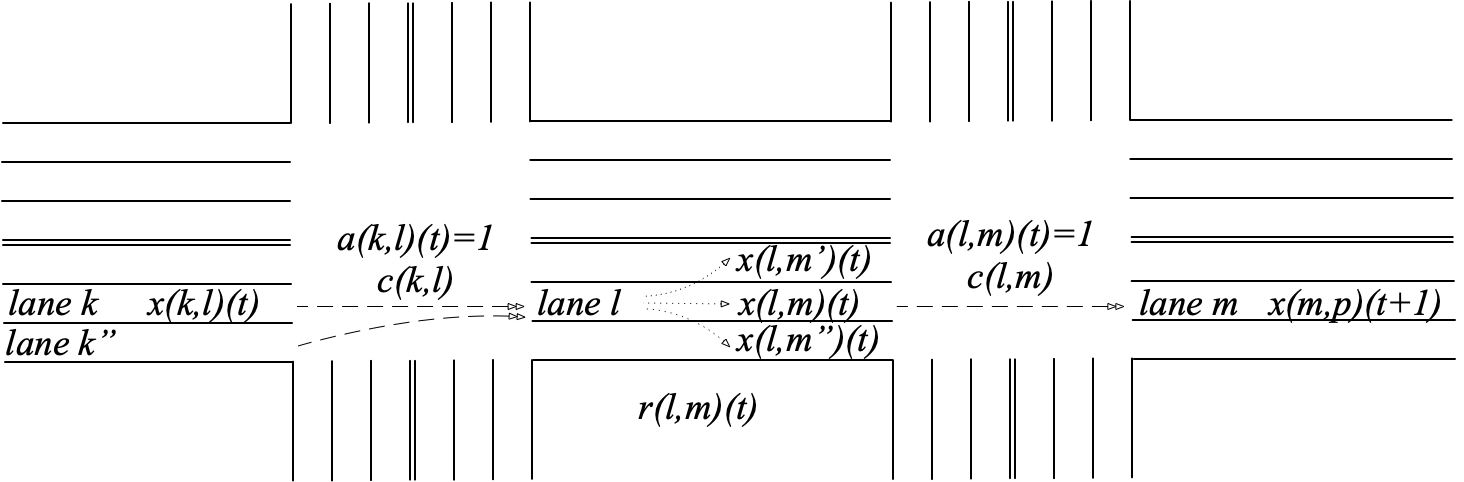
\includegraphics[width = 250pt]{figures/SFM1.png}
\caption{The transition of traffic movements}.
\label{fig:SFM}
\end{figure}


\subsection{Justification of State Design}

\subsubsection{Traffic movement process}
We now develop the equations of evolution of the state $X(t)$. For each $(l,m)$ and $t$, the queuing process consists of receiving and discharging. The evolution of  $x(l,m)$ is captured by the following equation:


\begin{equation}
\begin{split}
\label{eq:queue-process}
      & x(l,m)(t+1) \\
    = &\ x(l,m)(t) + \ \underbrace{ \Sigma_{k\in In_l} min[c(k,l)\cdot a(k,l)(t),\ x(k,l)]\cdot r(l,m)}_{receiving\ vehicles}\\
    - &\ \underbrace{ min\{c(l,m)\cdot a(l,m)(t),\ x(l,m)(t)\}\cdot \mathbf{1}(x(m)\le x_{max}(m))}_{discharging\ vehicles} \\
\end{split}
\end{equation}
where $In_l$ represent the set of links input to $l$. For the second term in Equation~\ref{eq:queue-process}, when $l$ is the receiving lane, up to $x(k,l)$ vehicles will move from queue $(k,l)$ if $a(k,l)(t)=1$ and they will join $(l,m)$ if $r(l,m)=1$
For the third term in Equation~\ref{eq:queue-process}, when traffic movement $(l,m)$ is actuated, i.e., $a(l,m)(t)=1$, up to $x(l,m)$ vehicles will leave queue $(l,m)$ and be routed to queue $(m,p)$ if there is no blockage on lane $m$, i.e., $x(m)\leq x_{max}(m)$, where $x_{max}(m)$ means the maximum capacity on lane $m$. 

\nop{
    \begin{equation}
    x(l,m)(t+1) = x(l,m)(t)+\delta(l,m)(t)
    \end{equation}
    where,
    \begin{align*}
    g_l(t) = min\{c(l,m)(t+1)\cdot a(l,m)(t),\ x(l,m)(t)\}\cdot \mathbf{1}(x(m)\le x_{max}(m)), \\ l\in\mathcal{L}, m\in Out_l
    \end{align*}
    
    \begin{align*}
    f_l(t) = \sum_k min[c(k,l)(t+1)\cdot a(k,l)(t),\ x(k,l)]\cdot r(l,m)(t+1)\\
     l\in \mathcal{L}, k\in In_l\\
    \end{align*}
}

For entry lanes of the system which have exogenous arrivals and no input lanes, the update equation is different: Equation~\ref{eq:queue-process} is modified to:
\begin{equation}
\begin{split}
\label{eq:queue-process-entry}
      & x(l,m)(t+1) \\
    = & x(l,m)(t) +  d(l,m)(t)\\
    - & min\{c(l,m)\cdot a(l,m)(t),\ x(l,m)(t)\}\cdot \mathbf{1}(x(m)\le x_{max}(m)) \\
\end{split}
\end{equation}

In~\cite{MP13}, the time frame $t\rightarrow t+1$ is assumed to be the lane travel time, which has 2 disadvantages: (1) It assumes all the lane travel time is the same no matter the link length. (2) It is resource consuming to take the traffic conditions $x(k,l)$ of nearby intersections. We can modify  the traffic movement equation at lane-level to segment-level.  The movement process on segment nearest to the intersection as following Equation~\ref{eq:queue-process-segnment}.
\begin{equation}
\begin{split}
\label{eq:queue-process-segnment}
      & x(l,m)_1(t+1) \\
    = &\ x(l,m)_1(t) + \ x(l,m)_2(t)\\
    - &\ min\{c(l,m)\cdot a(l,m)(t),\ x(l,m)_1(t)\}\cdot \mathbf{1}(x(m)\le x_{max}(m)) \\
\end{split}
\end{equation}
 where $x(l,m)_1$ is the number of vehicles on the segment, $x(l,m)_2$ is the number of vehicles on the outer segment.
 
Suppose the initial state $X(1)={x(l,m)(1)}$ is a non-negative bounded random variable. Since $A(t)={a(l,m)(t)}$ is a function of the current state $X(t)$, and since $c(l,m)$, $r(l,m)$, $d(l,m)(t)$ are all independent of $X(1),...,X(t)$, the process $X(t)$ is a \textit{\textbf{Markov chain}}. The transition probabilities of the chain $X(t)$ depends on the control policy.
 


\subsubsection{The defined state fully describes the system dynamic}
Through the lane movement evolution equation demonstrated above, the evolution of an individual intersection could be derived, which is a combination of the equations of all the connected links involved. Hence, for a single intersection $i$, 
\begin{itemize}
\item $c(l,m)$ the saturation flow rate is the constant physical feature of each lane.
\item $a(l,m)$ can be inferred from the agent's action.
% \item $X(i)$, $X(i')$ and $X(i'')$ should be provided to the local agent.
\item $x(l,m)_1$, $x(l,m)_2$ and $x(m)$ are provided to the local agent as in our state definition in Equation~\ref{eq:observation}.

\end{itemize}


\subsection{Justification of Reward Design}
\subsubsection{Our RL agent stabilizes the local traffic movement.}
Inspired by~\cite{MP13}, we first relax its assumptions about physical queue expansion in the arterial. Then the goal of our RL agents is proven to stabilize the queue length and thus maximizes the system throughput and minimizes the travel time of vehicles.

\theoremstyle{Definition}

\begin{definition}[Movement process stability] 
The movement process $X(t) = \{x(l, m)(t)\}$ is stable in the mean (and $u$ is a stabilizing control policy) if for
some $K<\infty$, Equation~\ref{eq:stability} holds. Movement stability in the mean implies that the chain is positive recurrent and has a unique steady-state probability distribution. $E$ denotes expectation. 
\begin{equation}
\label{eq:stability}
    \sum_{t=1}^{T}\sum_{(l,m)}E[x(l,m)(t)]<K,\quad\text{$\forall 
   T$.}
\end{equation}
\end{definition}

\begin{definition}[Max-pressure control policy~\cite{MP13}] 
At each period $t$, the agent selects the action with maximum pressure $\theta$ at every state $X$:
\begin{equation}
\tilde{A}^*(X) = argmax_{\tilde{A}\in \pmb{A}}\theta(\tilde{A}, X)
\end{equation}
where the pressure definition of each action $\tilde{A}\in\pmb{A}$ is shown as follows:
\begin{equation}
\theta(\tilde{A},X) = \sum_{l,m:a(l,m)=1}c(l,m)\cdot \tilde{w}(l,m)(X)
\end{equation}
where, $\tilde{w}(l,m)(X) = x(l,m)-\sum_{p\in Out_m}r(m,p)\cdot x(m,p)$ is the weight of each phase. In the following part, we denote quantities of max-pressure policy with hat, i.e., $\tilde{A}$ to differentiate with the quantities of RL policy without hat.
\end{definition}


\begin{theorem}
\label{theo:stable} Without considering the physical queue expansion, action $\tilde{A}^*$ selected by max-pressure control policy and action $A^*$ selected by our RL policy is stabilizing the system whenever the average demand is admissible, i.e., $d\in D^o$,
\end{theorem}

\textbf{Proof.}  For max-pressure control policy, Theorem 1 in~\cite{MP13} shows that given a time period $t=1,\ldots,T$ there exist $k<\infty$ and $\epsilon>0$ such that under $\tilde{A}^*$:
\begin{equation}
\label{eq:stability-proof}
\epsilon\cdot\frac{1}{T}\sum_{t=1}^TE[X(t)]\leq k + \frac{1}{T}\cdot E[X(1)]^2
\end{equation}
where $X(1)$ denotes the state when $t=1$. We include it here to stay self-contained.

For an optimal RL control policy $\pi$, the agent selects the action $A$ with maximum reward $Q^*$ at every state $X$, as stated in Equation~\ref{eq:q_max}
\begin{equation}
A^*(X) = argmax_{A\in \pmb{A}}Q^*(A, X)
\end{equation}

The difference between the pressure definition in RL reward and max-pressure is that our RL agent use the weighted pressure considering link storage capacity $x_{max}$ as Equation~\ref{eq:reward-detail}-b. The stability also holds by simply replacing $x(l,m)$ with $x(l,m)/x_{max}$.

\begin{theorem}
\label{theo:stable} Considering the physical queue expansion in the arterial environment, action $A^*$ selected by our RL policy is also stabilizing the movement.
\end{theorem}

Different from~\cite{MP13}, we establish the proof of Theorem~\ref{theo:stable} by relaxing the constraints of ignoring physical queue expansion in the arterial environment. Under arterial environment, there is:
\begin{itemize}
    \item The storage capacity $x_{max}$ on side street lane $m^{side}$ is assumed to be infinity, the second term in Equation~\ref{eq:reward-detail}-b is zero, thus we have $w(l,m^{side})=\frac{x(l,m^{side})}{x_{max}(l)}>0$.
    \item When the the downstream lane $m^{main}$ along the arterial is saturated, the second term in Equation~\ref{eq:reward-detail}-b is approximately 1 because of the queue expansion, thus phase weight $w(l,m^{main})\approx \frac{x(l,m^{main})}{x_{max}(l)} -1 < 0$. 
\end{itemize}

This means when we consider the physical queue expansion in the arterial, $w(l,m^{side}) > w(l,m^{main})$, the control policy will prohibit letting more vehicles pushing into the downstream intersection thus prevent the queue spill back and blocks the movements of vehicles in other phases. Accordingly, $K$ in Equation~\ref{eq:stability} is now set to be $K\leq x_{max}$, which constrains admissible demand to be $d\in D^{min,o} \subset D^o$. 


\subsubsection{RL is maximizing throughput and minimizing the travel time.} Given that the traffic movement process of each intersection is stable, the system is accordingly stable. In an arterial environment when there is no U-turn, it does not exists that both $x(m,l)$ and $x(l,m)$ are saturated, then the actions that RL agents take will not form grid lock or block the network, thus can efficiently utilize the green time. Within the given time period $T$, our RL agent can provides the maximum throughput, thus minimize the travel time of all vehicles within the system.






% !TEX root = main.tex
\section{Experiment}

\subsection{Experiment setting}


\subsubsection{Traffic network setting}
The experiments are run on CityFlow simulator, an open-source microscopic simulation package with flexible settings in network design, traffic simulation and traffic light control. 

% (Simulation of Urban Mobility)~\footnote{\url{http://sumo.dlr.de/index.html}}, an open-source microscopic simulation package with flexible settings in network design, traffic simulation and traffic light control. 


\paragraph{Simulating environments}
Without losing generality, we have three kinds simulating environments:
\begin{enumerate}[wide,noitemsep,topsep=0pt]
\item Arterial with 6 intersections. This part of experiments are conducted on an arterial with 6 four-leg intersections, see Figure~\ref{fig:Traffic-direc-pattern}. Each lane is 5 meters wide and 300 meters long. We use this environment to show the effectiveness of our method on synthetic uniform data and synthetic dynamic data with detailed explanation. For synthetic uniform data when there is no turning traffic, there is one lane on each direction. For synthetic dynamic data with turning traffic, there are 3 lane on each direction.

\begin{figure}[htb]
  \centering
	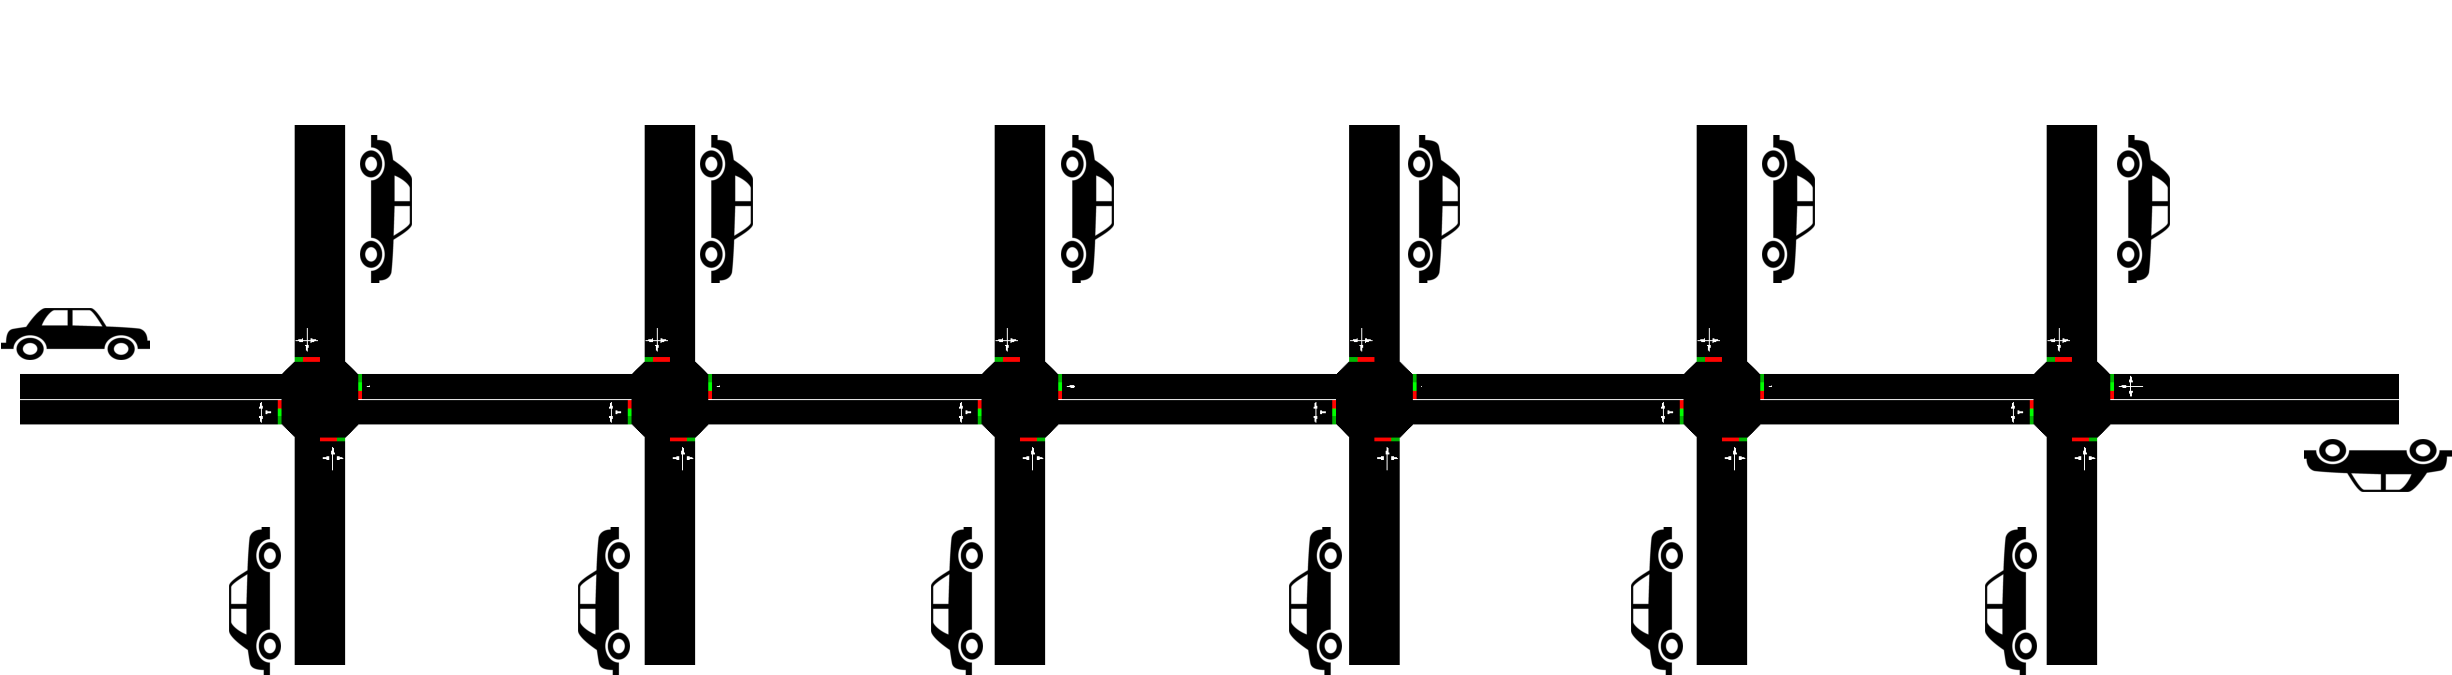
\includegraphics[width=\textwidth]{figures/arterial_6.pdf}
     \caption{Bidirectional traffic on an arterial with 6 intersections.}   
    \label{fig:Traffic-direc-pattern}
\end{figure}

% \item A heterogeneous arterial consisted of a 300-meters intersection and a 150-meters intersection. We use this environment to show the transferability of our model between heterogeneous intersections.
% \item Synthetic real-world scenario. By analyzing the traffic pattern of the data in Jinan, China and Hangzhou, China, the synthetic real data was generated to have the same statistical feature as the real-world data. The road network % we found out that, by a 24-hour time frame, the traffic patter of real-world data could be classified into 4 categories as it is shown in Figure~\ref{fig:Traffic-pattern}\Todo{draw pattern}. 

\item A real-world arterial in State College, Pennsylvania. This is an arterial with 5 intersections, each of which is a 4-leg intersection with 100 meters of both upstream and downstream sides. The arterial is one-way with two lanes, while the side streets have bi-directional traffic with one lane for each direction. Its arterial image is shown in~\ref{fig:real-intersection}(a).

\item A real-world arterial in Jinan, China. The arterial of Qingdao Road in Jinan, China has the same structure as aforementioned homogeneous arterial with 3 intersections. Its aerial image is shown in~\ref{fig:real-intersection}(b).

\end{enumerate}


\begin{figure*}[t!]
  \centering
  \begin{tabular}{c}
   \includegraphics[width=0.8\textwidth]{figures/case_beaver.png}\\ 
    \begin{tabular}[c]{@{}c@{}}(a) Beaver Avenue in State College, Pennsylvania, USA: \\a 5-intersection arterial with unidirectional traffic on the arterial\\ and bidirectional traffic on the side streets.\end{tabular}\\
   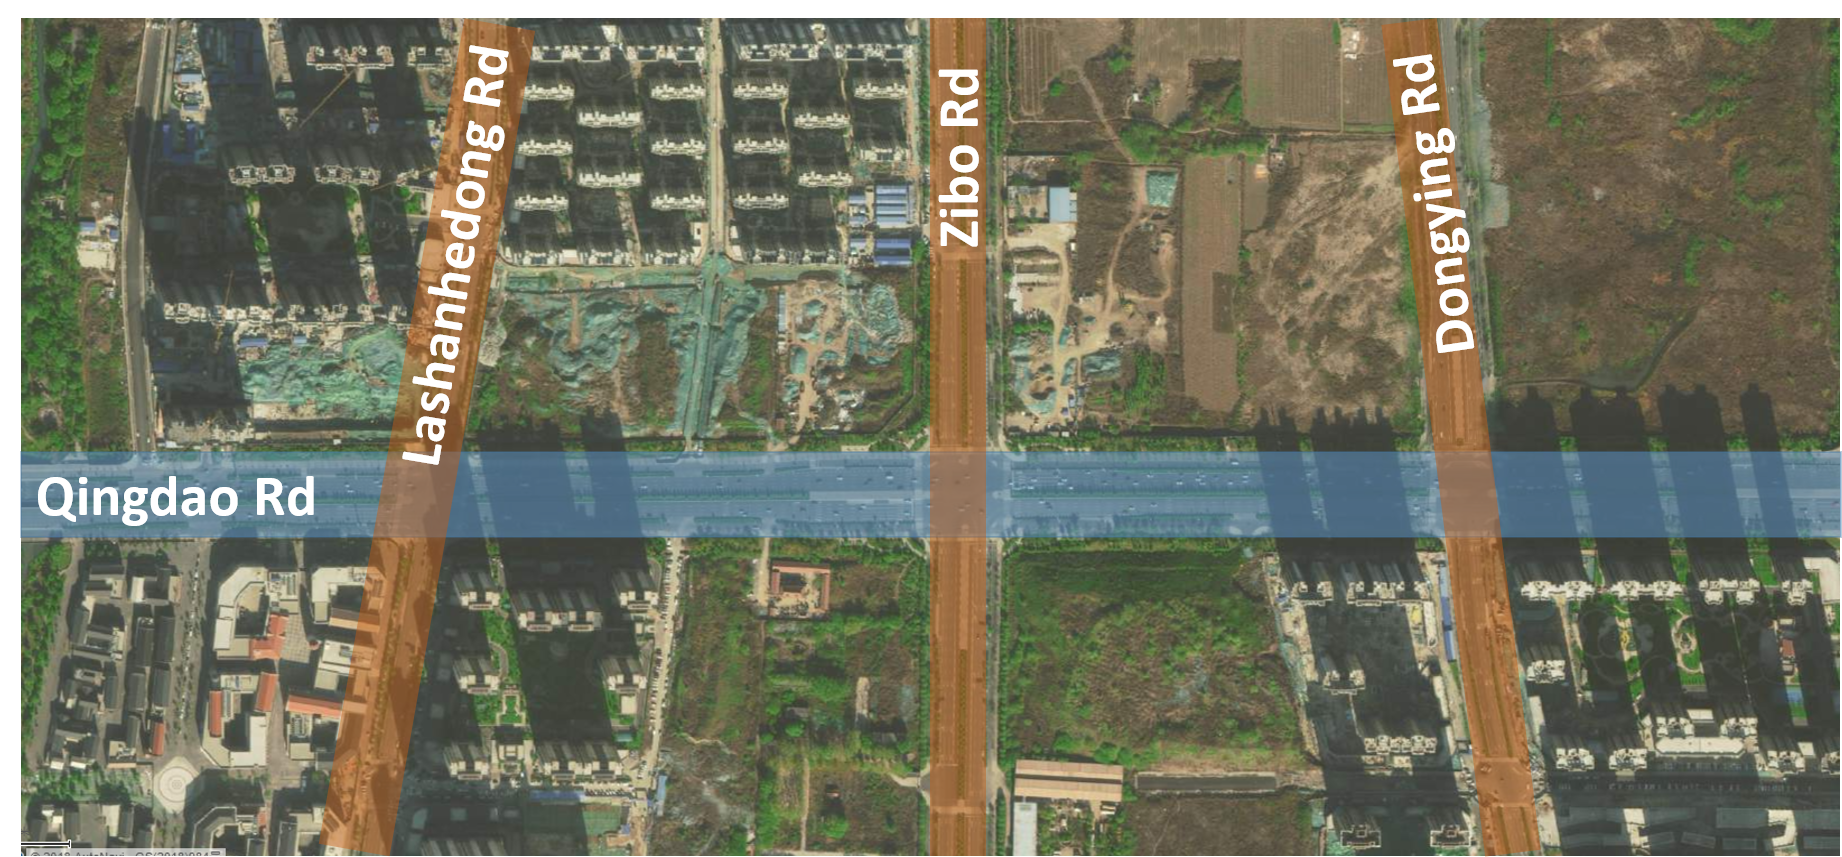
\includegraphics[width=0.8\textwidth]{figures/case_intersection_note.png}\\
   \begin{tabular}[c]{@{}c@{}}(b) Qingdao Road in Jinan, China:\\ a 3-intersection arterial with bidirectional traffic \\on both the arterial and the side streets.\end{tabular}\\
%   \begin{tabular}[c]{@{}c@{}}(a) Beaver Avenue in State College, Pennsylvania, USA: \\a 5-intersection arterial with unidirectional traffic on the arterial\\ and bidirectional traffic on the side streets.\end{tabular}&
%   \begin{tabular}[c]{@{}c@{}}(b) Qingdao Road in Jinan, China:\\ a 3-intersection arterial with bidirectional traffic \\on both the arterial and the side streets.\end{tabular}\\
   \end{tabular}
   
     \caption{Real-world arterials for experiment.}
    \label{fig:real-intersection}
\end{figure*}

The free-flow speed on the road segments in above settings is set to 40 kilometers/hour. The traffic light in this part of experiment contains four phases: (1) WE-straight (green on WE straight going lane), (2) SN-straight (red on SN straight going lane), (3) WE-left (green on WE left turning lane), (4) SN-left (green on SN left turning lane) Every time the phase switches, a 5-second combined yellow and all-red time are followed to clear the intersection. Note that phase (3) and phase (4) would be disabled for when there is no turning traffic.
 
\subsubsection{Evaluation metric}
Following existing studies, we use the most frequently used measure, i.e., average travel time, to evaluate the performance (other measures show similar performance and are not shown here due to space limit):

\begin{itemize}
% \item \textbf{Queue length} ($Queue$) calculates average queue length over time, where the
% queue length at time $t$ is the sum of queue lengths over all approaching lanes. 
% \item  \textbf{Pressure} calculates the average pressure as defined above on each intersections at each time step. The pressure denotes the queuing stability inside the road network.
\item  \textbf{Travel time} calculates average travel time the vehicles spent on approaching lanes (in seconds). This is the most frequently used measure for traffic signal performance in transportation field.
\end{itemize}

% We also use \textbf{number of training rounds to converge} to measure the effectiveness of the training process of reinforcement learning agents.  

\subsubsection{Compared methods}
We compare our model with the following methods. It should be noted that all methods except the offsets of $\FT$ are carefully tuned and their best results are reported~\footnote{The codes including parameter settings is available at authors' website}. 

\begin{itemize}[wide,noitemsep,topsep=0pt]

\item \textbf{\FT}: Fixed-time with random offset~\cite{Roess2011t}. Each phase has fixed time of 15 seconds. For uni-directional traffic, there are only 2 phases (WE-straight, SN-straight). For traffic with turning vehicles, there are 4 phases. 

% The optimal cycle length of each intersection is calculated by close form solution as Equation~\ref{eq:cycle-length} given by the Webster's theory~\cite{Roess2011t}. The phase split percentage is equivalent with the percentage between the demand for a designated phase and total demand. The offsets are randomly selected to mimic an arterial with all traffic signals progressing independently. 

% \begin{equation}
% \label{eq:cycle-length}
% C_{min}=\frac{N\times{l}}{1-(\frac{v_c}{3600/h})}
% \end{equation}
% where $N$ is the number of phases in one cycle; $l$ is the lost time of a signal phase; $v_c$ is the maximum summation of volumes of critical lanes; $h$ headway of saturated traffic flow. 

\item \textbf{\Greenwave}: Green wave coordination on the arterial for unidirectional traffic~\cite{Roess2011t}. All intersections share the same cycle length, which is the maximum value of the cycle length for individual intersections calculated using Equation~\ref{eq:cycle-length}. The phase split percentage is equivalent with the percentage between the demand for a designated phase and total demand. Offsets between intersections are equivalent to the free-flow travel time between two consecutive intersections. %Vehicles traveling in the direction of green wave can benefit from a progressive cascade of green light without stopping at any intersections. 
\begin{equation}
\label{eq:cycle-length}
C_{min}=\frac{N\times{l}}{1-(\frac{v_c}{3600/h})}
\end{equation}
This is the most classical method in transportation field to implement coordination. However, \Greenwave is only an optimal solution for unidirectional and uniform traffic on the arterial. 

\item \textbf{\Maxpressure}: Max pressure control policy ~\cite{varaiya2013max}. \Maxpressure maximizes network throughput. The phase is determined by the pressure defined by the algorithm.

% optimal offsets to maximize the weighted combination of bandwidths for both directions of traffic along the arterial~\cite{little1981maxband}. The cycle length and phase split is calculated in the same  way as \Greenwave.

\item \textbf{\Deeplight} is an individual deep reinforcement learning approach proposed in \cite{wei2018intellilight}. This method does not consider context information.
%  \Deeplight is a single intersection control model that uses a representation of the local traffic information as state and reward function.

In addition to the baseline methods, we also consider several variations of our model.

\item \textbf{\SDeeplight}: By changing the state of \Deeplight from number of vehicles on each approaching lanes to the number of vehicles on each segment of lanes (coming vehicle distribution), with this more delicate state design, the agents will have more information than \Deeplight agents.

% \item \textbf{\SNDeeplight} The state is further modified as same as our proposed state, i.e., number of lane segments' vehicles on both approaching lanes and exiting lanes.

\item \textbf{\SNDeeplight} Our proposed method. 

Note that all the learning methods share the same neural network structure.


% \item \textbf{\NIPS} is a coordinated reinforcement learning approach for multi-intersection control~\cite{VaOl16}. Specifically, the coordination is achieved by designing a coordination graph and the joint local Q-function is defined on two intersections directly. Thus, this method can only optimize the joint action between two intersections.

\end{itemize}

% We denote our proposed method as \textbf{\PressLight}. We also compare a variation of our proposed method without network sharing, denoted as \textbf{\MDeeplight}.  

\subsection{Datasets}

\subsubsection{Synthetic data}

In the first part of the experiment, we use eight different configurations for synthetic traffic data, detailed in Table~\ref{tab:synthetic-table}. Note that all the traffic flow is uni-directed and there is no turning traffic. All the traffic is uniform, the demand in Table~\ref{tab:synthetic-table} is equal to critical lane volume ratios in the system, which is practically used to determine the phase split in field.

% Under each configuration, we have two variants on traffic: through traffic only (denoted as $\withoutturn$) and traffic with turns (20\% turning right and 20\% left, denoted as $\withturn$).Since all the traffic is uniform and evenly split among lanes, the demand in Table~\ref{tab:synthetic-table} is equal to critical lane volume ratios in the system, which is practically used to determine the phase split in field.

% \begin{table}[tbp!]
% \begin{center}
% \caption{Configurations for synthetic traffic data}
% \label{tab:synthetic-table}
% \begin{tabular}{c|c|c|c|c}
% \toprule
%  & \begin{tabular}[c]{@{}c@{}}Demand\\pattern \end{tabular}&\begin{tabular}[c]{@{}c@{}}
%   Arterial \\demand (cars/h)\end{tabular} &  \begin{tabular}[c]{@{}c@{}}Side-road\\ demand (cars/h) \end{tabular} &\begin{tabular}[c]{@{}c@{}}  Config\\ \#\end{tabular} \\ \hline
% %   \multicolumn{5}{*}{uniform}\\
% %   \hline
%  \multirow{4}{*}{Uniform} 
%  &\multirow{2}{*}{Unidirectional} & {300}    & 180   &1  \\ \cline{3-5} 
%                  &                & {700}    & 420   &2  \\\cline{2-5}
%  &\multirow{2}{*}{Bidirectional}  & {300}    & 180   &3  \\ \cline{3-5} 
%                   &               & {700}    & 300   &4  \\\bottomrule
%  \multirow{4}{*}{Dynamic} 
%  &\multirow{2}{*}{Flat} & {300}    & 180   &5  \\ \cline{3-5} 
%                   &               & {700}    & 420   &6  \\\cline{2-5}
%  &\multirow{2}{*}{Fluctuated}  & {300}    & 180   &7  \\ \cline{3-5} 
%                   &              & {700}    & 300   &8  \\\bottomrule
% \end{tabular}
% \end{center}
% \end{table}
\begin{table}[tbp!]
\begin{center}
\caption{Configurations for synthetic traffic data}
\label{tab:synthetic-table}
\begin{tabular}{c|c|c|c}
\toprule
  \begin{tabular}[c]{@{}c@{}}Demand\\pattern \end{tabular}&\begin{tabular}[c]{@{}c@{}}
  Arterial \\demand (cars/h)\end{tabular} &  \begin{tabular}[c]{@{}c@{}}Side-road\\ demand (cars/h) \end{tabular} &\begin{tabular}[c]{@{}c@{}}  Config\\ \#\end{tabular} \\ \hline
  % \multicolumn{5}{*}{uniform}\\
  % \hline
\multicolumn{4}{c}{Uniform}  \\
\hline
 \multirow{2}{*}{Unidirectional} & {300}    & 180   &1  \\      \cline{2-4} 
                                & {700}    & 420   &2  \\      \cline{1-4}
 \multirow{2}{*}{Bidirectional}  & {300}    & 180   &3  \\      \cline{2-4} 
                               & {700}    & 300   &4  \\      \bottomrule
\multicolumn{4}{c}{Dynamic}  \\
                 \hline
 \multirow{2}{*}{Flat} & {300}    & 180   &5  \\               \cline{2-4} 
                                & {700}    & 420   &6  \\     \cline{1-4}
 \multirow{2}{*}{Fluctuated}  & {300}    & 180   &7  \\        \cline{2-4} 
                                & {700}    & 300   &8 \\     \bottomrule
\end{tabular}
\end{center}
\end{table}

\paragraph{Traffic $\withoutturn$}
We test our method under through traffic $\withoutturn$ in the experiment for the following reasons: 

\begin{itemize}
\item Under this situation, we can verify whether the proposed technique has reached the optimal solution. In general, the problem of finding a globally optimal solution for agents with partial information is known to be intractable~\cite{bernstein2002complexity}. But under synthetic uniform unidirectional traffic without turning, the optimal solution is known ($\Greenwave$ on the arterial). So we only need to verify whether $\PressLight$ has reached the same state as $\Greenwave$ to know whether our method has converged to the optimal solution.
\item The through-only traffic do exist in real world, especially for arterials and highways. For example, the US Highway-1 near Monmouth Junction prohibits left-turn and always allows right-turn traffic.
\end{itemize}

\paragraph{Synthetic dynamic data to have the same statistical feature as real-world data in Jinan and Hangzhou, China} This dataset was synthesized after a statistical analysis of real-world traffic pattern in Jinan and Hangzhou. Specifically, we care the turning ratio, the maximum traffic volume and the ratio of arterial traffic flow and side-street flow most. This parameters are carefully chosen to imitate reality. As a result, all the vehicles on approaching lanes  will have 10\% of possibility to turn left and 30\% turning right. The maximum traffic volume is set to be 700 for over-saturated scenario and 300 for under-saturated scenario. The ratios of arterial traffic flow and side-street flow are chosen to be 0.3 and 0.6 respectively.

% \paragraph{Traffic $\withturn$}
% We also test our method under traffic with turns for a more general setting. All the vehicles on approaching lanes will have 20\% of possibility to turn left and 20\% turning right. For unidirectional settings, the traffic on side streets might only have left turns or right turns with 20\% of overall traffic.

\subsubsection{Real-world data}

% \subsubsection{Real-world data}
\paragraph{Traffic profile in State College, Pennsylvania, the United States} This traffic dataset was collected during a traffic signal re-timing project in State College, Pennsylvania, USA. Traffic movement counts were manually collected for each intersection in the downtown area for morning, midday and afternoon peak hours. The data were aggregated into hourly volumes for left turn, through and right turn movements. We use the traffic volumes of intersections on Beaver Avenue, an one-way arterial in downtown State College. Its aerial image is shown in Figure~\ref{fig:real-intersection}(a).

\begin{center}
\begin{table*}[]
\centering
\caption{Performance on synthetic data in the arterial with 6 intersections}
\label{tab:synthetic-result}
% Please add the following required packages to your document preamble:
% \usepackage{multirow}
% Please add the following required packages to your document preamble:
% \usepackage{multirow}
% Please add the following required packages to your document preamble:
% \usepackage{multirow}
\begin{tabular}{|c|c|c|c|c|c|c|c|c|}
\hline
Measure                  & \multicolumn{8}{c|}{Average travel time}                                        \\ \hline
\multirow{2}{*}{Config.} & \multicolumn{4}{c|}{Synthetic uniform} & \multicolumn{4}{c|}{Synthetic dynamic} \\ \cline{2-9} 
                         & 1       & 2        & 3       & 4       & 5       & 6        & 7       & 8       \\ \hline
\FT                          & 70.17        & 124.56   & 70.17   & 124.56  & 93.29   & 325.48   & 109.50  & 246.25  \\ \hline
\Greenwave                       & 62.36    & 75.88    & 65.31   & 79.93   & 98.39   & 263.36   & 124.09  & 286.85  \\ \hline
\Maxpressure                       & 63.29  & 161.60   & 66.39   & 147.88  & 74.30   & 262.26   & 82.37   & 225.60  \\ \hline
\Deeplight                      & 64.45     & 86.86    & 67.09   & 102.73  & 65.07   & 233.17   & 66.77   & 258.33  \\ \hline
\PressLight                     & 62.33     & 75.73    & 59.42   & 74.98   & 59.96   & 160.48   & 61.34   & 184.51  \\ \hline
\end{tabular}
\end{table*}
\end{center}

\begin{center}
\begin{table*}[tp!]
\centering
\caption{Comparison with variants of our methods}
\label{tab:variants-result}
\begin{tabular}{|c|c|c|c|c|c|c|c|c|}
\hline
\multicolumn{9}{|c|}{Variants of our methods}                                                                                                                                                                                     \\ \hline
Measure                      & \multicolumn{8}{|c|}{Average travel time}          \\ \hline
\multicolumn{1}{|c|}{Config} & \multicolumn{1}{c|}{1} & \multicolumn{1}{c|}{2} & \multicolumn{1}{c|}{3} & \multicolumn{1}{c|}{4} & \multicolumn{1}{c|}{5} & \multicolumn{1}{c|}{6} & \multicolumn{1}{c|}{7} & \multicolumn{1}{c|}{8} \\ \hline
\Deeplight     & 64.45                  & 86.86                  & 67.09                  & 102.73                 & 65.07                  & 233.17                 & 66.77                  & 258.33                 \\ \hline
\SDeeplight                   & 62.54                  & 81.03                  & 59.89                  & 92.26                  & 59.06                  & 207.98                 & 60.23                  & 191.86                 \\ \hline
\SNDeeplight     & 62.70 &	81.17	& 59.92	&95.86	&61.20	&200.28	&61.76	&196.34\\ \hline

IRL+n  & 62.84 &	83.63 &	61.49 &	90.68 &	67.32 &	201.56 &	68.47 &	281.21 \\ \hline

\PressLight    & 62.33                  & 81.19                  & 59.90                  & 84.71                  & 59.96                  & 160.48                 & 61.34                  & 184.51                 \\ \hline
\end{tabular}
\end{table*}
\end{center}

% % \begin{table}[]
% \begin{center}
% \begin{table*}[tp!]
% \caption{Performance on synthetic data in the arterial with homogeneous intersections}
% % \label{tab:synthetic-result}
% \begin{tabular}{|l|l|l|l|l|l|l|l|l|}
% \hline
% Measure & \multicolumn{4}{l|}{Average travel time} & \multicolumn{4}{l|}{Average pressure} \\ \hline
% Config. & 1        & 2       & 3        & 4        & 1       & 2       & 3       & 4       \\ \hline
% \multicolumn{9}{|c|}{3 INTERSECTIONS}                                                      \\ \hline
% FT      & 66.86    & 57.08   & 146.78   & 117.17   & 0.34    & 0.45    & 4.94    & 6.07    \\ \hline
% GW      & 62.80    & 53.71   & 67.50    & 65.28    & 0.18    & 0.28    & 0.87    & 2.01    \\ \hline
% MP      & 65.87    & 57.52   & 73.16    & 80.40    & 0.48    & 0.57    & 1.28    & 12.42   \\ \hline
% IRL     & 61.38    & 52.62   & 69.8     & 65.42    & 0.05    & 0.05    & 0.77    & 1.53    \\ \hline
% NIPS    &          &         &          &          &         &         &         &         \\ \hline
% NEW     & 60.48    & 52.5    & 66.43    & 65.56    & 0.05    & 0.05    & 0.43    & 1.42    \\ \hline
% \multicolumn{9}{|c|}{10 INTERSECTIONS}                                                     \\ \hline
% FT      & 111.31   & 78.78   & 180.78   & 129.20   & 0.24    & 0.29    & 1.87    & 2.94    \\ \hline
% GW      & 95.74    & 69.64   & 100.68   & 80.74    & 0.15    & 0.24    & 0.71    & 1.67    \\ \hline
% MP      & 95.37    & 73.44   & 112.39   & 128.92   & 0.29    & 0.49    & 1.42    & 4.57    \\ \hline
% IRL     & 93.78    & 66.86   & 110.14   & 91.01    & 0.05    & 0.02    & 0.96    & 2.18    \\ \hline
% NIPS    &          &         &          &          &         &         &         &         \\ \hline
% NEW     & 91.52    & 67.45   & 92.26    & 103.44   & 0.06    & 0.07    & 0.76    & 2.35    \\ \hline
% \end{tabular}
% \label{tab:result_syn}
% \end{table*}
% \end{center}

% \begin{center}
% \begin{table*}[tp!]
% \caption{Performance on synthetic data in the arterial with homogeneous intersections}
% \label{tab:synthetic-result}
% \centering
% \begin{tabular}
% {p{0.05\textwidth}p{0.03\textwidth}p{0.03\textwidth}p{0.03\textwidth}p{0.03\textwidth}p{0.03\textwidth}p{0.03\textwidth}p{0.03\textwidth}p{0.03\textwidth}|p{0.035\textwidth}p{0.035\textwidth}p{0.035\textwidth}p{0.035\textwidth}p{0.035\textwidth}p{0.035\textwidth}p{0.035\textwidth}p{0.035\textwidth}}
% \toprule
% Measure & \multicolumn{8}{c|}{$Queue$}& \multicolumn{8}{|c}{$Time$} \\
% \hline
% Config. & 1     & 2     & 3     & 4     & 5    & 6      & 7     & \multicolumn{1}{c|}{8}     & 1      & 2     & 3      & 4      & 5      & 6      & 7      & 8      \\
% \hline
% \multicolumn{17}{c}{2-intersection arterial under traffic $\withoutturn$ (through traffic only)}                                                                                                                                               \\
% \hline
% \FT      & 0.62  & 0.91  & 2.09   & 3.07  & 1.26 & 1.83   & 4.20   & \multicolumn{1}{c|}{6.24}  & 52.65  & 49.17 & 62.86  & 58.43  & 52.65  & 49.17  & 62.85  & 58.43  \\
% \Greenwave      & 0.59  & 0.99  & 1.31  & \textbf{2.3}   & 1.19 & 1.98   & 4.25  & \multicolumn{1}{c|}{6.24}  & 51.77  & 49.01    & \textbf{51.92}  & \textbf{52.29}  & 51.79  & 49.01  & 60.27  & 56.53  \\
% \Max & -     & -     & -     & -     & 1.89 & 1.69   & 2.21  & \multicolumn{1}{c|}{\textbf{5.72}}  & -      & -     & -      & -      & 57.36  & 47.81  & 53.88  & 56.57  \\
% \Deeplight     & 0.70   & 0.70   & 1.28  & 4.81  & 1.55 & 1.61   & 2.60   & \multicolumn{1}{c|}{7.86}  & 54.53  & 47.43 & 53.01  & 63.57  & 53.79   & 47.24  & 52.05  & 58.75  \\
% \NIPS    & 0.56  & 0.80   & 1.59  & 2.77  & \textbf{0.73} & 1.79 & 21.65 & \multicolumn{1}{c|}{10.00}    & 51.31  & 47.5  & 52.06  & 52.55  & 50.33  & 54.42  & 272.76 & 67.46  \\
% \PressLight    & \textbf{0.41}  & \textbf{0.54}  & \textbf{1.00}     & 2.80   & 0.83 & \textbf{0.92}   & \textbf{1.95}  & \multicolumn{1}{c|}{6.23}  & \textbf{50.03}  & \textbf{45.73} & 52.13  & 53.83  & \textbf{50.11}  & \textbf{45.52}  & \textbf{51.94}  & \textbf{56.18}  \\
% \hline
% \multicolumn{17}{c}{3-intersection arterial under traffic $\withoutturn$ (through traffic only)}                                                                                                                                               \\
% \hline
% \FT      & 0.98  & 0.52  & 2.12  & 3.09  & 1.96 & 1.04   & 4.23  & \multicolumn{1}{c|}{6.27}   & 65.91  & 57.5  & 79.96  & 69.3   & 65.9   & 57.53  & 79.93  & 69.32  \\
% \Greenwave      & 0.53  & 0.92  & 1.15  & \textbf{2.1}   & 1.06 & 1.85   & 4.5   & \multicolumn{1}{c|}{6.42}  & 63.85  & 56.73 & \textbf{63.86}  & \textbf{60.02}  & 63.86  & 56.71  & 76.49  & 66.77  \\
% \Maxband & -     & -     & -     & -     & 1.54 & 2.09   & \textbf{2.00}  & \multicolumn{1}{c|}{\textbf{5.48}}  & -      & -     & -      & -      & 67.45  & 57.87  & 67.52  & \textbf{64.37}  \\
% \Deeplight     & 0.8   & 0.55  & 1.55  & 4.13  & 1.05 & 1.16   & 2.72  & \multicolumn{1}{c|}{9.28}  & 67.41  & 52.90  & 67.56  & 69.48  & 63.31  & 53.52  & 66.52  & 70.38  \\
% \NIPS    & 0.563 & 0.346 & 2.88  & 2.92 & 1.19 & 1.39   & 3.77  & \multicolumn{1}{c|}{26.11} & 64.45  & 53.02 & 80.05  & 142.09 & 63.79  & 53.94  & 69.29  & 109.49 \\
% \PressLight    & \textbf{0.35}  & \textbf{0.43}  & \textbf{0.89}  & 2.36  & \textbf{0.72} & \textbf{0.76}   & 2.03  & \multicolumn{1}{c|}{6.22}  & \textbf{61.94}  & \textbf{52.54} & 64.08  & 62.17  & \textbf{62.50}   & \textbf{52.33}  & \textbf{65.06}  & 65.27  \\
% \hline
% \multicolumn{17}{c}{4-intersection arterial under traffic $\withoutturn$ (through traffic only)}                                                                                                                                               \\
% \hline
% \FT      & 0.56  & 0.87  & 2.13  & 3.11  & 1.12 & 1.75   & 4.25  & \multicolumn{1}{c|}{6.81}   & 75.04  & 62.61 & 92.31  & 76.31  & 75.04  & 62.62  & 92.31  & 76.31  \\
% \Greenwave      & 0.5   & 0.94  & 1.06  & \textbf{2.17}  & 1.01 & 1.88   & 4.53  & \multicolumn{1}{c|}{6.9}   & 72.75  & 61.78 & \textbf{72.71}  & \textbf{66.07}  & 72.76  & 61.79  & 87.79  & 74.42  \\
% \Maxband & -     & -     & -     & -     & 1.79 & 2.38   & 1.84  & \multicolumn{1}{c|}{\textbf{5.66}}  & -      & -     & -      & -      & 79.44  & 64.91  & 76.39  & 72.66  \\
% \Deeplight     & 0.6   & 0.58  & 1.63  & 9.51  & 0.79 & 0.92   & 3.3   & \multicolumn{1}{c|}{9.62}  & 75.57  & 58.83 & 80.42  & 190.5  & 70.74  & 57.18  & 78.02  & 78.54  \\
% \NIPS    & 0.54  & 0.60   & 1.28  & 5.99  & 0.56 & 1.18   & 8.59  & \multicolumn{1}{c|}{29.86} & 72.94  & 59.44 & 91.23  & 77.75  & 69.95  & 56.74  & 95.21  & 197.8  \\
% \PressLight    & \textbf{0.32}  & \textbf{0.40}   & \textbf{0.87}  & 2.47  & \textbf{0.50}  & \textbf{0.70}    & \textbf{1.61}  & \multicolumn{1}{c|}{6.53}  & \textbf{70.68}  & \textbf{56.92} & 73.23  & 67.13  & \textbf{70.37}  & \textbf{56.67}  & \textbf{73.07}  & \textbf{72.30}   \\
% \hline
% \multicolumn{17}{c}{10-intersection arterial under traffic $\withoutturn$ (through traffic only)}                                                                                                                                               \\
% \hline
% \FT      & 1.24  & 1.71  & 2.12  & 3.10  & 2.65 & 3.57   & 4.22  & \multicolumn{1}{c|}{6.16}  & 131.51 & 96.23 & 136.36 & 101.21 & 131.88 & 96.45  & 136.61 & 101.33 \\
% \Greenwave      & 0.36  & 0.60  & 0.79  & \textbf{1.61}  & 1.28 & 2.19   & \textbf{1.48}  & \multicolumn{1}{c|}{\textbf{3.40}}  & 103.24 & 76.62 & 105.98 & 81.65  & 112.46 & 84.22  & 103.88 & 86.53  \\
% \Maxband & -     & -     & -     & -     & 1.91 & 2.48   & 1.67  & \multicolumn{1}{c|}{4.96}  & -      & -     & -      & -      & 108.89 & 78.73  & 103.32 & 84.11  \\
% \Deeplight     & 0.65  & 0.47  & 1.71  & 3.55  & 0.57 & 0.79   & 2.31  & \multicolumn{1}{c|}{7.60}  & 93.90  & 72.41 & 108.27 & 97.08  & 87.96  & 72.12  & 96.73  & 97.70  \\
% \NIPS    & 0.67  & 3.47  & 16.04 & 17.00 & 1.33 & 2.52   & 24.65 & \multicolumn{1}{c|}{31.91} & 109.53 & 82.59 & 248.72 & 263.04 & 109.85 & 144.72 & 212.51 & 206.55 \\
% \PressLight    & \textbf{0.34}  & \textbf{0.29}  & \textbf{0.75}  & 1.86  & \textbf{0.47} &  \textbf{0.65}  &  1.54 & \multicolumn{1}{c|}{4.43}      & \textbf{88.56}  & \textbf{70.45} & \textbf{88.56}  & \textbf{80.27}  &    \textbf{40.66} &   \textbf{70.78}  & \textbf{90.74}  & \textbf{83.41} \\ 

% \hline
% \multicolumn{17}{c}{4-intersection arterial under traffic $\withturn$ (with left and right turn traffic)}                                                                                                                                               \\
% \hline
% \FT      & 1.07 & 1.52 & 1.63 & 2.47 & 2.16 & 3.18   & 5.27 & 4.55 & 76.68 & 70.02 & 76.97 & 71.37 & 77.51 & 71.54 & 91.93 & 85.41 \\
% \Greenwave      & 0.49 & 0.85 & 0.81 & 1.81 & 1.24 & 2.20   & 1.55 & 2.27 & 67.26 & 62.77 & 67.20 & 65.51 & 67.26 & 62.97 & 67.20 & 65.51 \\
% \Maxband & -    & -    & -    & -    & 1.43 & 2.09   & 1.73 & 3.71 & -     & -     & -     & -     & 71.20 & 71.74 & 65.93 & 77.75 \\
% \Deeplight     & 0.33 & 0.69 & 0.67 & 1.13 & 0.66 & 1.6    & 1.3  & 1.31 & 64.99 & 61.68 & 66.67 & 62.41 & 65.28 & 63.02 & 68.68 & 67.43 \\
% \NIPS    & 0.33 & 0.67 & 0.88 & 1.05 & 0.86 & 228.00 & 5.08 & 1.99 & 65.69 & 61.98 & 68.43 & 62.82 & 67.59 & 75.50 & 84.87 & 69.01 \\
% \PressLight    & \textbf{0.28} & \textbf{0.63} & \textbf{0.56} & \textbf{1.00} & \textbf{0.53} & \textbf{1.44}   & \textbf{1.05} & \textbf{1.03} & \textbf{64.60} & \textbf{61.56} & \textbf{66.24} & \textbf{62.29} & \textbf{64.78} & \textbf{62.85} & \textbf{65.34} & \textbf{66.81} \\

% \bottomrule
% \end{tabular}
% \label{tab:result_syn}
% \end{table*}
% \end{center}


\paragraph{Surveillance camera data in Jinan, China}
The real-world dataset are collected by road-side surveillance cameras in Jinan, China over the time period from 08/01/2016 to 08/31/2016. In every second, the camera gathers records about the vehicles passing though the camera consisting time, camera ID, direction and vehicle plate ID. By analyzing these records with camera locations, the trajectories of vehicles are recorded.
We use the time of vehicles entering these intersections as traffic flow for experiments. We feed this real-world traffic into SUMO as on-line experiments. We select an arterial with 3 intersections, as shown in Figure~\ref{fig:real-intersection}(b). The reason we select this case is because all these 3 intersections have 4-way surveillance cameras that describe the comprehensive view of the traffic conditions.

\subsection{Performance on synthetic data}

\subsubsection{Comparison with state-of-the-art methods} 


% \begin{figure}[htb]
%   \centering
% 	\includegraphics[width=0.48\textwidth]{figures/offset_draft.pdf}
%      \caption{Bidirectional traffic on an arterial with 6 intersections.}   
%     \label{fig:case-study}
% \end{figure}

% \begin{figure*}[thb]
%   \centering
%   \begin{tabular}{cc}
%   \includegraphics[width=0.42\textwidth]{figures/offset_draft.pdf} &
% %   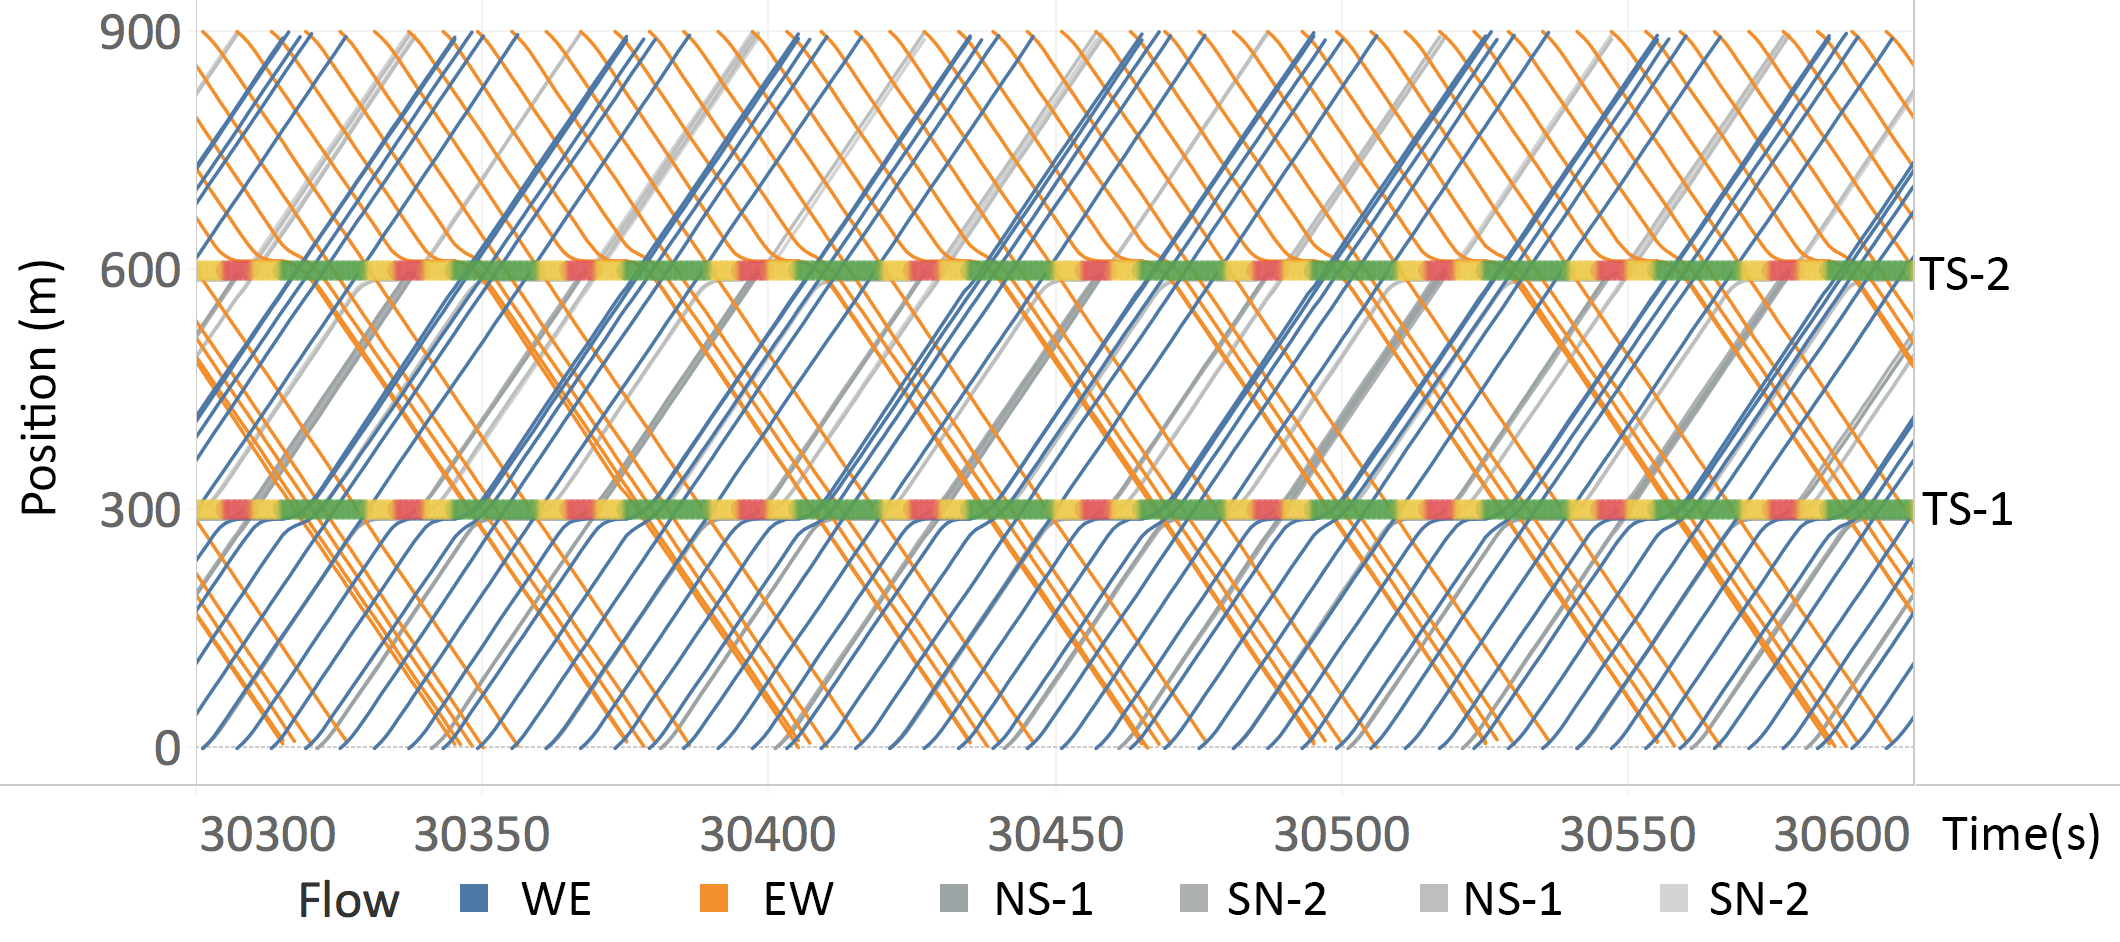
\includegraphics[width=0.45\textwidth]{figures/case_study_2_bi.png} \\
%   \begin{tabular}[c]{@{}c@{}}(a) Synthetic data configuration 1 on a 4-intersection arterial\end{tabular}&
% %   \begin{tabular}[c]{@{}c@{}}(b) Synthetic data configuration 5 on a 2-intersection arterial\end{tabular}\\
%   \end{tabular}
% \caption{Space-time diagrams with signal timing plans to illustrate the learned unidirectional (a) and bidirectional (b) green waves from synthetic data. The green-yellow-red bands represent the learned signal plans on \WE. Each line in space-time diagram stands for one vehicle's trajectory. The trajectory of a vehicle in the green wave will be a straight sloped line in the space-time diagram.}
%     \label{fig:case-study}
% \end{figure*}

We first compare our method with four other baselines under 8 configurations on an arterial with 6 intersections. From Table~\ref{tab:synthetic-result}, we can see that: 
% Note that \Maxband only works when there is bidirectional traffic. From Table~\ref{tab:synthetic-result}, we can see that: 

1) Our proposed method \PressLight can achieve the best performance for most of the settings compared with state-of-the-arts. \Greenwave is designed for unidirectional uniform traffic. Hence, under configuration 1 and 2, \Greenwave achieves best travel time. Our proposed method could achieve similar performance. This demonstrates that,even without explicit coordination, our RL agents can learn the coordination implicitly. For bidirectional or dynamic traffic (configuration 3-8), \Maxpressure is more capable. However, as a rule based control, the inherit parameters within \Maxpressure is hard to tune, thus emphasizing the effectiveness of our learning based agents. \Deeplight also achieves good performance for all of the settings and our method is always better, which verifies the effectiveness of our proposed state and reward design.

% Some baselines perform well on certain setting (e.g., \Greenwave achieves good travel time under configuration 1 and 2 and \Maxpressure is more capable dealing with bi-directional traffic (configuration 3-8), our proposed methods could always achieve similar or better performances. This also demonstrates that,even without explicit coordination, our RL agents can learn the coordination implicitly. Compared with individual control (\IRL), it is shown that coordination could be learned with our new design of sate and reward of RL agents. 

% including the method with explicit coordination strategies (\Greenwave) \nop{ \Maxband and \NIPS}, as is shown in Table~\ref{tab:synthetic-result}. This demonstrates that, even without explicit coordination, our RL agents can learn the coordination implicitly. Although some baselines perform well on certain setting (e.g., \Greenwave achieves good travel time under configuration 1 and 2, while our method also achieves similar performances), they perform badly in other configurations. This is because those methods are designed for these settings, e.g., \Greenwave is designed for unidirectional uniform traffic, \Maxband is designed for bidirectional uniform traffic, and \NIPS is designed for two-intersection regional control.
% {\color{blue}maxpressure is better than greenwave for bidirectional traffic}

2) For dynamic traffic, which is a more realistic, our method always achieves the best performance. In Table~\ref{tab:synthetic-result}, for configuration 5-8, our method steadily outperform all other baselines in terms of travel time. Is shows that learning agents is able to adapt to changing traffic. 

3)When the traffic volume grows to larger (configuration 4, 6 and 8), our method becomes much better than other baselines. This is because our agents, inspired by \Maxpressure, consider to balance the traffic pressure on all of the intersections with the road network.

In summary, our method \PressLight shows better performance under different configurations.

% When there is turning traffic $\withturn$, which is a more realistic setting, our method also outperform other methods. This is mainly because \Greenwave and \Maxband only consider the traffic that travels along the arterial, and \NIPS only optimizes the joint action for two intersections. In summary, our method \PressLight shows better performance under different configurations.

% \subsection{Performance on dynamic data}

\subsubsection{Comparison with variants of our proposed method}  
We compare several variation of our method to validate the effectiveness of state and reward design. Table~\ref{tab:variants-result} shows the performance of variants of our proposed method. First we can see that by adding context information, it immediately boost the performance of individual control agents for all settings. It is able to achieve similar best performance under unidirectional and traffic with small flow (configuration 1, 2, 3, 5 and 6). However, for over-saturated bidirectional traffic scenario, optimizing queue length of each agents individually would ignore the congestion on neighboring intersections. Hence, inspired by \Maxpressure, the reward is modified from minimizing queue length to minimizing the difference of queue lengths of all the approaching lanes and queue lengths of exiting lanes. To make sure that the agent is able to observe traffic distribution on exiting lanes, vehicle distribution on exiting lanes are added into state design. It turns out that by balancing the queues for each intersection, it further boost the performance under over-saturated traffic. In addition, another variants, \SNDeeplight, with same state but no modification on reward is investigated too. The result shows that given more state information would not significantly boost the performance, but somehow interfere the convergence speed thus resulting in no improvement compared to \SDeeplight.

% to optimize pressure, by which the queue 
% without information of exiting approaches, the agents may fail
% But it does not achieve best when the traffic volumes grow larger.

% \Todo{state that reward and state information is necessary}
% 3>2>1>0
% We compare a variation of our method to validate the effectiveness of sharing the network.
% Results in Table~\ref{tab:entropy} show that \PressLight shows a better stability than \MDeeplight under both homogeneous and heterogeneous situations. This is because the network parameters are shared transferred from a similar intersection agent model serves as a good guidance to help the model converge faster as well as build up its robustness. For arterials with heterogeneous intersections, the values of entropy of all settings for both \MDeeplight and \PressLight are higher than those in homogeneous settings, indicating the structure of network does affects the convergence of RL agents.


\subsubsection{Our proposed reward - pressure is correlated with travel time}  
To show the correlation of our proposed reward--pressure and average travel time, we draw a figure to show the process of convergence by plotting the average reward (pressure) each round with average travel time each round. Figure~\ref{fig:convergence} illustrates the correlation between pressure and travel time.

% \Todo{justifying reward figure -- convergence figure}

\begin{figure}[t!]
\centering
  \begin{tabular}{c}
   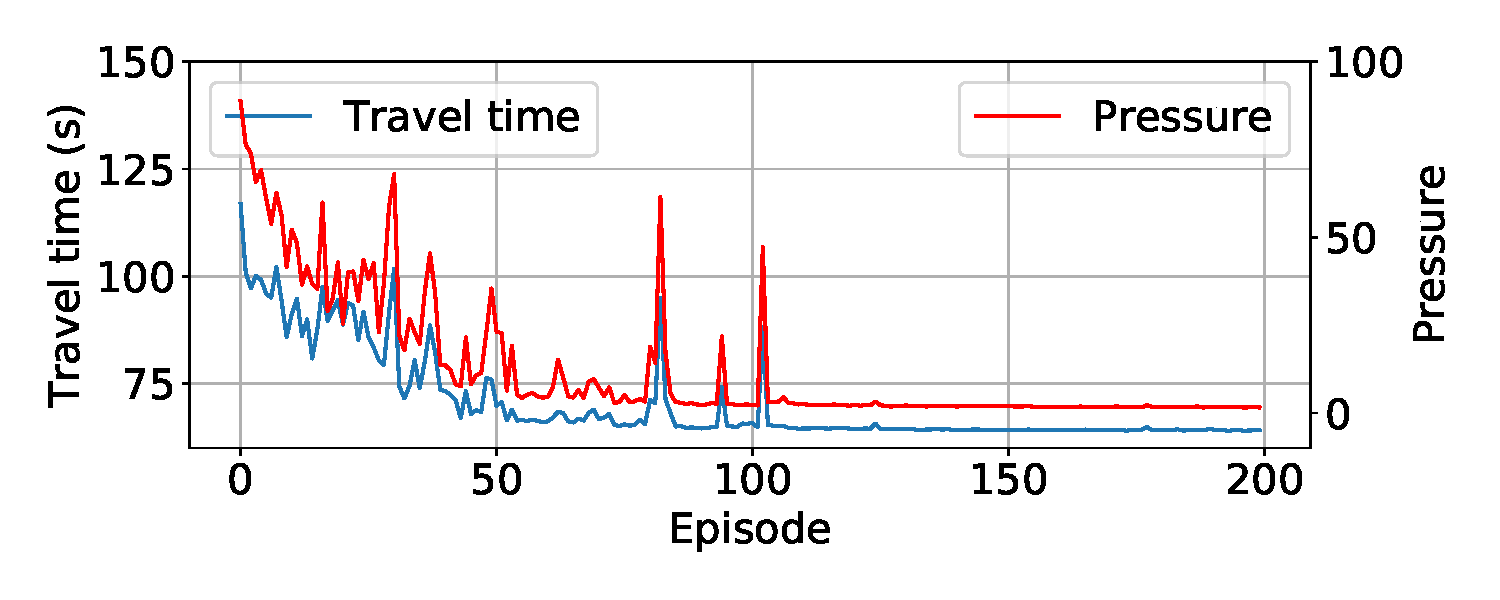
\includegraphics[width=0.8\textwidth]{figures/converg.pdf} \\
   \end{tabular}
     \caption{Correlation of average duration and pressure.}
    \label{fig:convergence}
\end{figure}



% \Todo{if we have time}
\subsubsection{Number of intersections}
% \Todo{table here}
We employ our model where we vary the number of intersections from 6 to 10. Table~\ref{tab:number_of_intersections} illustrates the performance of configuration 1-4 for our model and \Maxpressure. The conclusion could be drawn that our model could achieve better performance even when the number of intersections grows.

\begin{table}[]
\centering
\caption{Performance in a 10-intersection arterial}
\label{tab:number_of_intersections}
\begin{tabular}{|c|c|c|c|c|}
\hline
Measure & \multicolumn{4}{c|}{Average travel time} \\ \hline
Config. & 1        & 2        & 3       & 4        \\ \hline
\Maxpressure      & 68.78    & 129.63   & 68.78   & 129.63   \\ \hline
\textbf{\PressLight}    &      \textbf{66.27}    &     \textbf{88.88}     & \textbf{67.18}   & \textbf{79.61}    \\ \hline
\end{tabular}
\end{table}


\begin{table}[]
\centering
\caption{Performance on real-world data}             
\begin{tabular}{|c|c|c|}
\hline
Config                             & Beaver               & Jinan          \\ \hline
Measure                            & Travel time          & Travel time    \\ \hline
\FT                                 & 336.29          & 317.40    \\ \hline
\Greenwave                                 & 332.06          & 370.30    \\ \hline
\Maxpressure                                 & 222.90          & 567.06    \\ \hline
\Deeplight                                & 338.52          & 58.18          \\ \hline
% \multicolumn{3}{|c|}{Variants of our methods}                              \\ \hline
% \SDeeplight                         & 151.70          & 56.12          \\ \hline
\textbf{\PressLight} & \textbf{92.00} & \textbf{54.87} \\ \hline
\end{tabular}
\label{tab:real_result}
\end{table}

% \begin{table}[t!]
% \centering
% \caption{Performance on real-world data}
% \begin{tabular}
% {p{0.06\textwidth}p{0.06\textwidth}p{0.08\textwidth}p{0.001\textwidth}p{0.06\textwidth}p{0.06\textwidth}}
% \toprule
%         & \multicolumn{2}{c}{\begin{tabular}[c]{@{}c@{}}Beaver  Avenue\\ in State College\end{tabular}} & & \multicolumn{2}{c}{\begin{tabular}[c]{@{}c@{}}Qingdao Road\\ in Jinan\end{tabular}} \\ \hline
%         & $Queue$   & \multicolumn{1}{l|}{$Time$\ \ \ } & & $Queue$   & $Time$ \\ \hline
% \FT      & 1.83    &  \multicolumn{1}{l|}{58.63} & & 7.85  & 159.20 \\
% \Greenwave & 1.24   &  \multicolumn{1}{l|}{48.56}& & 5.73  & 140.71  \\
% \Deeplight     & 0.7 &  \multicolumn{1}{l|}{38.29}&  & 2.80   & 95.86  \\
% \Maxband & -      &  \multicolumn{1}{l|}{- }&        & 1.84   & 97.97  \\
% \NIPS    & 1.83   &  \multicolumn{1}{l|}{37.28}&     & 1.39   & 97.66  \\  \hline
% \MDeeplight     &  0.62 & \multicolumn{1}{l|}{37.01}&  & 1.75 & 89.23  \\
% \PressLight     & \textbf{0.27}  &  \multicolumn{1}{l|}{\textbf{36.30}}&  & \textbf{1.34} & \textbf{86.25}  \\   
% \bottomrule
% \end{tabular}
% \label{tab:real_result}
% \end{table}


\subsubsection{Green wave learned from RL agents}

\begin{figure}[htb]
  \centering
	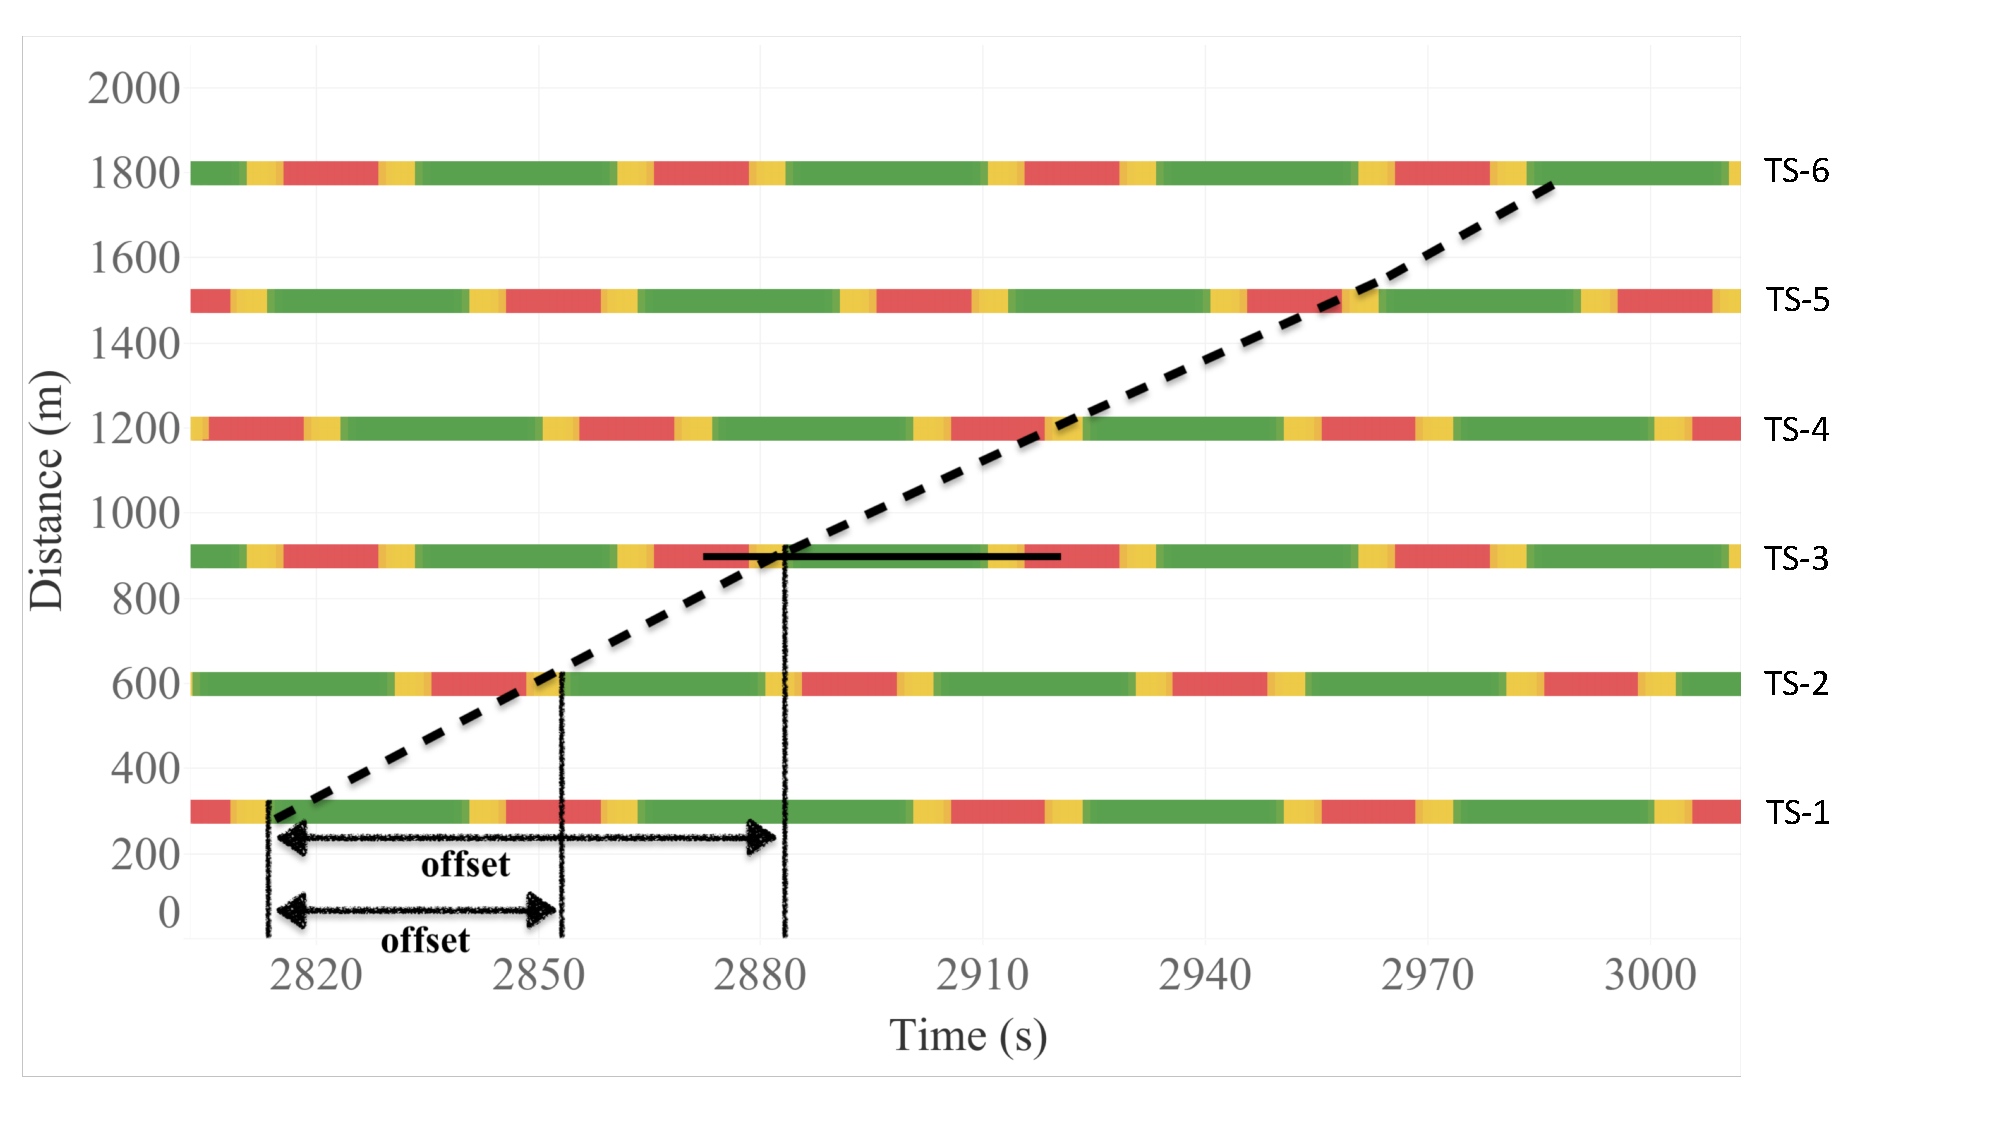
\includegraphics[width=0.8\textwidth]{figures/offset.pdf}
     \caption{Offsets between intersections learnt by RL agents}   
    \label{fig:case-study}
\end{figure}

To validate that our method can learn an optimal solution under ideal conditions (configuration 2), we use the synthetic setting where conventional coordination method \Greenwave can form a green wave for traffic along the arterial and is an optimal solution as stated in ~\cite{Roess2011t}. The \Greenwave offset $\Delta$ equals to the block length $l$ between two consecutive intersections divided by free-flow speed $v$, and the optimal phase split is equal to the percentage between the demand for a designated phase and total demand. In our experiments, $l\approx 300$ m, $v\approx 10$ m/s, hence, the optimal offset should be $\Delta\approx 30$ s, and the optimal phase split should be 1:0.6 (Green-\WE : Red-\WE). However, the min action time of our agents is 10s, hence the result of the control policy learned does not fit into the theoretically calculated optimal solution. Specifically, we use time-space diagrams to show trajectories of vehicles and phase plans of traffic signal controllers, as it is shown in Figure~\ref{fig:case-study}. 

\begin{figure*}[t!]
  \centering
  \begin{tabular}{c}
   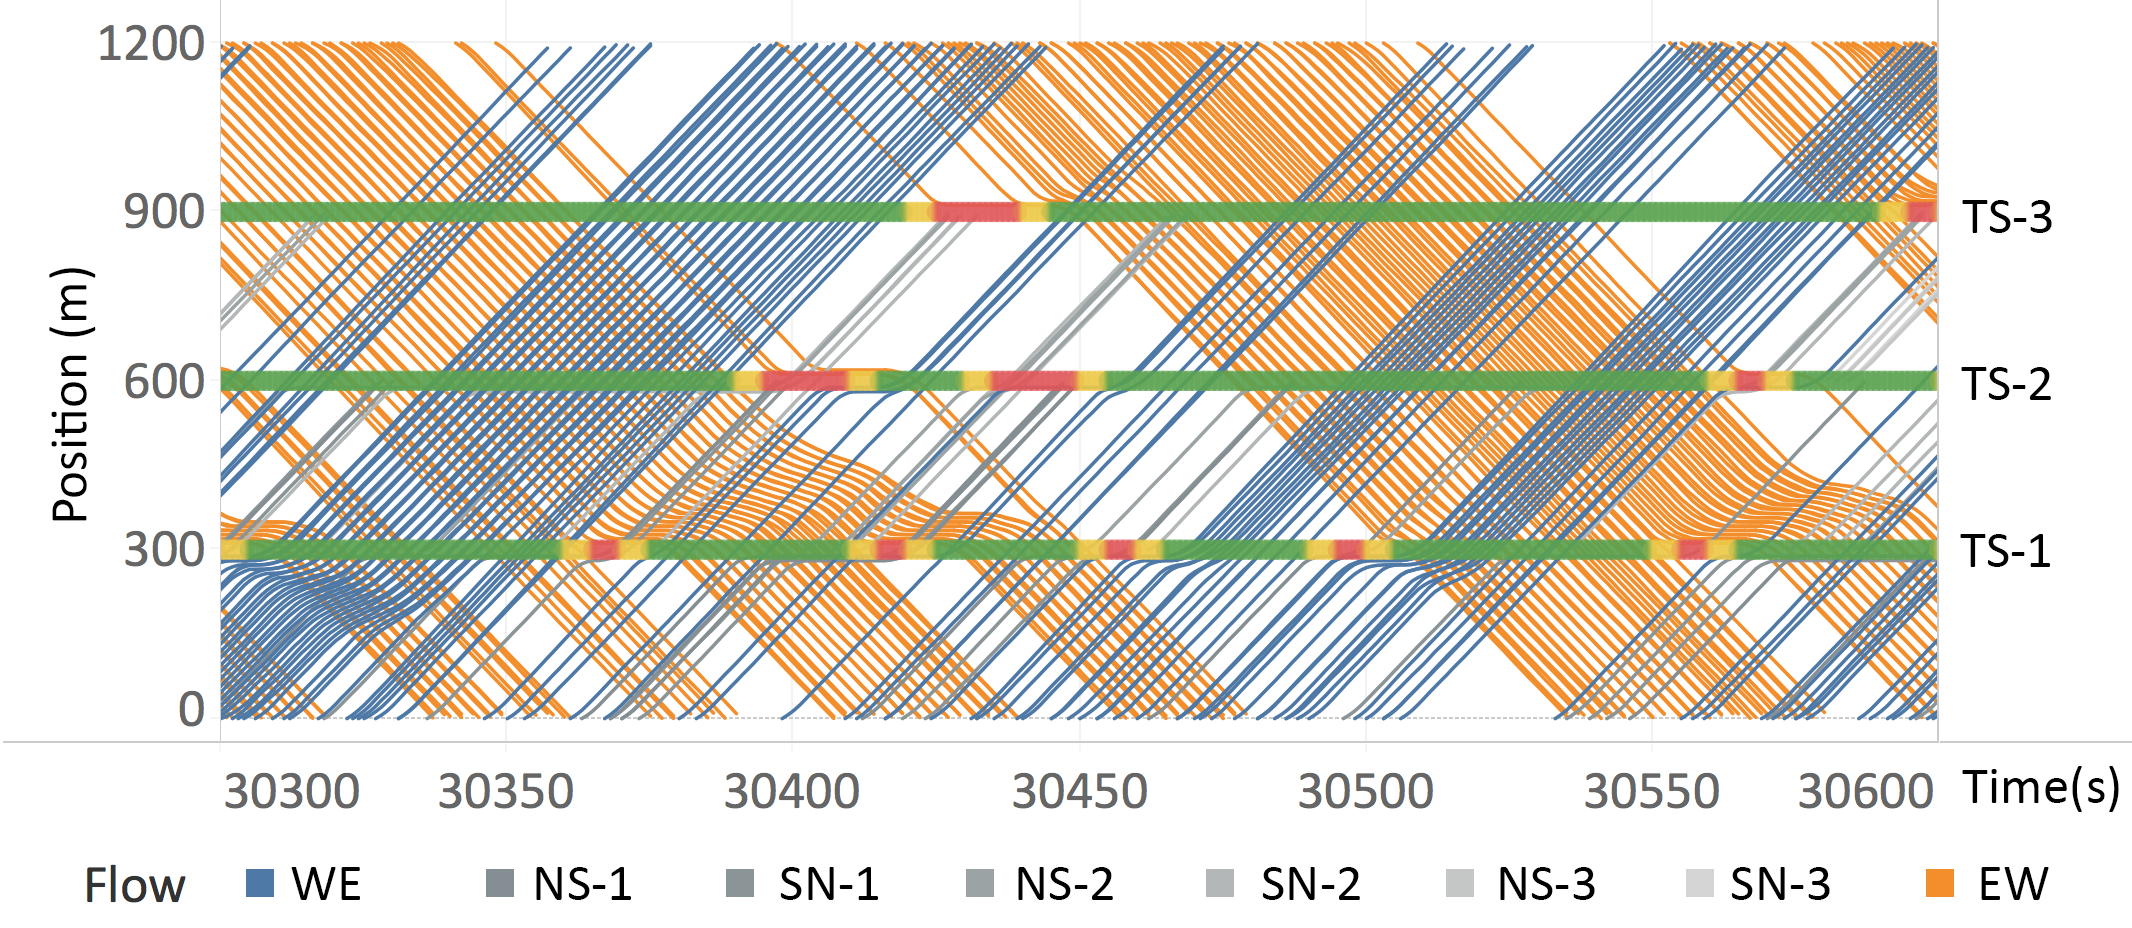
\includegraphics[width=0.85\textwidth]{figures/case_study_real_1.png} \\
   \end{tabular}
     \caption{Space-time diagram with signal timing plan to illustrate the learned coordination strategy from real-world data on the arterial of Qingdao Road in the morning (around 8:30 a.m.) of August 6th.}
    \label{fig:case-study-real}
\end{figure*}

A time-space diagram is drawn with time on the horizontal axis and distance (from a reference point, here we use the westernmost point on the arterial as the reference point) on the vertical axis, exampled as Figure~\ref{fig:case-study} and~\ref{fig:case-study-real}. A learned offset was visualized in the diagram. Vehicles move across 6 traffic lights with distance from 0 to 1800. Hence, the dotted line in the Figure~\ref{fig:case-study} could be seen as a possible vehicle trajectory. The slope indicates free flow speed. Traffic signal offset is indicated and it is approximately 25s or 30s between every 2 traffic signals.

% Vehicle trajectories are plotted on the time-space diagram and the difference in distance over time (distance divided by time, or change in $y$ divided by $x$) represents the speed or a sloped line on the diagram. The trajectories for vehicles on the arterial always move left to right along with time, and as shown the distance traversed can be either eastbound (bottom to top of the diagram) or westbound (top to bottom). Vehicles can have a positive or negative slope that indicates the movements on the street network. Stopped vehicles (no change in distance) are shown as horizontal lines. Vehicles traversing green waves (always at their free-flow speed) will be straight sloped lines.


% Vehicle trajectories are plotted on the time-space diagram and the difference in distance over time (distance divided by time, or change in $y$ divided by $x$) represents the speed or a sloped line on the diagram. The trajectories for vehicles on the arterial always move left to right along with time, and as shown the distance traversed can be either eastbound (bottom to top of the diagram) or westbound (top to bottom). Vehicles can have a positive or negative slope that indicates the movements on the street network. Stopped vehicles (no change in distance) are shown as horizontal lines. Vehicles traversing green waves (always at their free-flow speed) will be straight sloped lines.


For unidirectional traffic, as is shown in Figure~\ref{fig:case-study}(a), our method not only forms a green wave for vehicles on the arterial, but also learns the optimal cycle length and phase split, which is 50s and 1:0.6 (Green-\WE:25s Red-\WE:15s Yellow-phase:5+5). 

% For bidirectional traffic, while it is hard to form a green wave because it has strict requirements on the road structures (i.e., the blocks along the arterial to be identical) and on the relationships between cycle length and free-flow speed, our method can also learn the bidirectional {\Greenwave} with zero offsets and the optimal cycle length equals to the free-flow travel time between consecutive intersections, as is shown in Figure~\ref{fig:case-study}(b). This experiment further proves the capability of out RL model to learn bidirectional {\Greenwave} signal settings without any prior knowledge, providing maximum green bandwidth for both directions ~\cite{Roess2011t}.


\subsection{Performance on real-world data}
\subsubsection{Comparison of different methods} In this section, we compare our method with baseline methods on real-world data. The overall results are shown in Table~\ref{tab:real_result}.
From Table~\ref{tab:real_result}, we can see that our method \PressLight achieves the best result over all the compared methods in terms of queue length and travel time, with a relative improvement of 61\% and
3\% in the setting of Beaver Avenue, and 4\% and 12\% in the setting of Qingdao Road correspondingly over the best baseline method.
% In addition, \PressLight outperforms \MDeeplight steadily, indicating the effectiveness of transferred knowledge.


\subsubsection{Green wave learned from RL agents}
In this section,
we make observations on the policies we learned from the real
data for the arterial of Qingdao Road (\WE and \EW ) at Lashanhedong Road (\SN-1 and \NS-1), Zibo Road (\SN-2 and \NS-2) and Dongying Road (\SN-3 and \NS-3) during the morning peak hour (around 8:30 a.m.) on August 6th. 


A time-space diagram is drawn with time on the horizontal axis and distance (from a reference point, here we use the westernmost point on the arterial as the reference point) on the vertical axis, exampled as Figure~\ref{fig:case-study-real}. 

Vehicle trajectories are plotted on the time-space diagram and the difference in distance over time (distance divided by time, or change in $y$ divided by $x$) represents the speed or a sloped line on the diagram. The trajectories for vehicles on the arterial always move left to right along with time, and as shown the distance traversed can be either eastbound (bottom to top of the diagram) or westbound (top to bottom). Vehicles can have a positive or negative slope that indicates the movements on the street network. Stopped vehicles (no change in distance) are shown as horizontal lines. Vehicles traversing green waves (always at their free-flow speed) will be straight sloped lines.

In Figure~\ref{fig:case-study-real}, most of the blue and orange lines are straight, indicating most vehicles on main road (including both \WE and \EW direction), are not stopped by red lights. This indicates that our method can automatically form a green wave under the real-world traffic.


% !TEX root = main.tex
\section{Conclusion}
In this chapter, we propose a novel RL method for multi-intersection traffic signal control on the arterials. We conduct extensive experiments using both synthetic and real-world experiments and demonstrate the superior performance of our method over state-of-the-art methods. Specifically, we draw a connection between reinforcement learning with conventional transportation control methods. It is the first time there exists a RL model automatically achieving coordination along a arterial without explicit priori knowledge. 
 
 We also acknowledge the limitations of our current approach and possible future directions could be the following. First, we can extend the tested corridor with more intersections, which will involve more complicated yet more realistic settings. The authors would expect increased computational cost while introducing more agents, however, our RL model is still elegant as there is no need for further model modifications. Secondly, our model is currently tested on a simulation environment, thus the feedbacks of control is also simulated. A field study is needed to validate our method in the real-world environment. Lastly, since the real-world traffic condition is a compound of cars, motorcycles, bikes and pedestrians, a comprehensive coordination between different parties should also be investigated. 
\chapter{PressLight: Learning Max Pressure Control for Signalized Intersections in Arterial Network}
\label{chap:presslight}
\section{Overview}
\label{sec:intro}


Traffic signals coordinate the traffic movements at the intersection and a smart traffic signal control algorithm is the key to transportation efficiency. Traffic signal control remains an active research topic because of the high complexity of the problem. The traffic situations are highly dynamic, thus require traffic signal plans to be able to adjust to different situations.

Recently, people start to investigate reinforcement learning (RL) techniques for traffic signal control. Several studies have shown the superior performance of RL techniques over traditional transportation approaches~\cite{Wier00,AbPK03,ALUK10,AbMB13,VaOl16,wei2018intellilight}. The biggest advantage of RL is that it directly learns how to take the next actions by observing the feedback from the environment after previous actions. 

\begin{figure}[]
\centering
\begin{tabular}{ccc}
   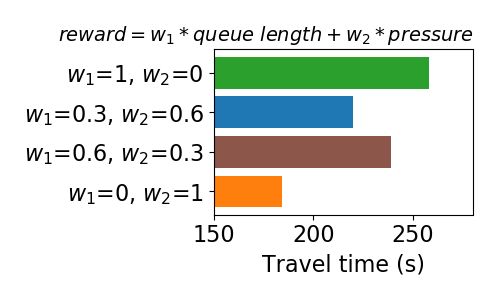
\includegraphics[width=0.45\textwidth]{figures/intro_1.png}&
   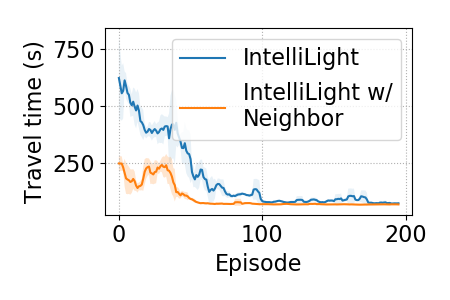
\includegraphics[width=0.4\textwidth]{figures/intro_0.png}\\
   \begin{tabular}[c]{@{}c@{}}(a) Performance w.r.t. reward\end{tabular} &
   \begin{tabular}[c]{@{}c@{}}(b) Convergence w.r.t. state\end{tabular} \\ 
   \end{tabular}
\label{fig:intro}
\caption{Performance of RL approaches is sensitive to reward and state. (a) A heuristic parameter tuning of reward function could result in different performances. (b) The method with a more complicated state (\LIT~\cite{ZXZF+19} w/ neighbor) has a longer learning time but does not necessarily converge to a better result. }
\label{fig:intro}
\vspace{-3mm}
\end{figure}

One major issue of current RL-based traffic signal control approaches is that the setting is often heuristic and lacks proper theoretical justification from transportation literature. This often results in highly sensitive performance w.r.t. the setting and leads to a long learning process. We elaborate on this issue by examining two fundamental elements in RL setting: reward and state.

First, various reward designs have been proposed in the literature. The reason is that travel time, the ultimate objective, is hard to optimize directly. Travel time is a long-term reward depending on a sequence of actions, thus the effect of one action can hardly be reflected in terms of travel time. People thus choose short-term rewards like queue length or delay to approximate the travel time~\cite{hua19survey}. So the reward function is often defined as a weighted sum of these terms~\cite{VaOl16,BPT14,ElAb10,ElAA13,wei2018intellilight}. However, as shown in Figure~\ref{fig:intro}(a), tuning the weights on these terms could lead to largely different results in terms of travel time. Some literature~\cite{ZZXW+19} discusses how to define the reward by connecting with the existing transportation method, but they only focus on controlling a single intersection. In this chapter, we focus on the multi-intersection control scenario. 

Second, existing RL methods have a trend of using more complicated state representation. Recent studies use visual images to describe the full traffic situation at the intersection~\cite{VaOl16,wei2018intellilight}, which results in the dimension of the state in the scale of thousands. In the single intersection scenario,~\cite{ZZXW+19} reveals that additional information is not always helpful. Similar conclusions can also be found in the multi-intersection scenario. As shown in Figure~\ref{fig:intro}(b), complicated state definitions increase the learning time and may not necessarily bring significant gain. Note that we are not claiming that additional information is always not helpful. The choice of the state depends on the reward setting. Based on the reward design of \LIT~\cite{ZZXW+19}, neighboring information is not necessary in the case we show in Figure~\ref{fig:intro}(b). The question is, could we justify theoretically how much information is enough in state definition in order to optimize the reward function?


\begin{figure}
    \centering
    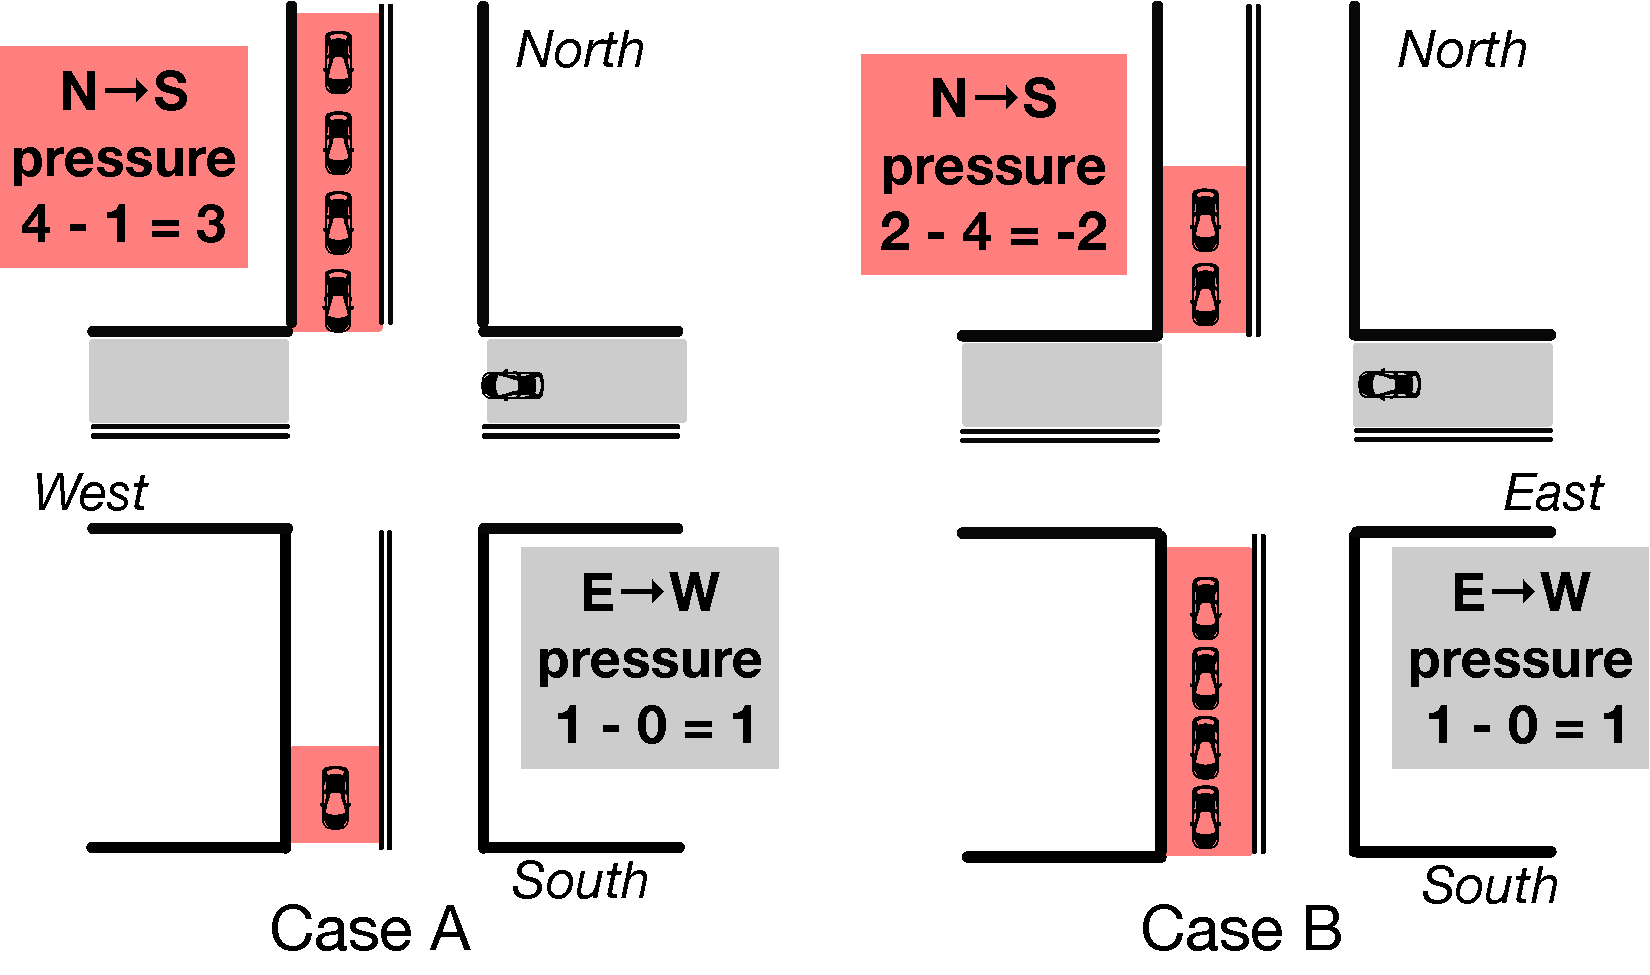
\includegraphics[width=0.8\textwidth]{figures/Maxpressure.pdf}
    \caption{Illustration of max pressure control in two cases. In Case A, green signal is set in the North$\rightarrow$South direction; in Case B, green signal is set in the East$\rightarrow$West direction.}
    \label{fig:pressure}
    \vspace{-2mm}
\end{figure}

The challenges we face in RL motivate us to look for support from transportation. In transportation literature, max pressure (MP) control is one of the state-of-the-arts in traffic signal control~\cite{MP13-adaptvie,MP13}. The key idea of MP is to minimize the ``pressure'' of an intersection, which can be loosely defined as the number of vehicles on incoming lanes minus the number of vehicles on outgoing lanes. Figure~\ref{fig:pressure} illustrates the concept of pressure. By setting the objective as minimizing the pressure of intersections, MP is proved to maximize the throughput of the whole road network\footnote{Maximizing throughput equals to minimizing travel time under certain conditions and minimizing travel time is the final goal for most traffic signal control problems.}. However, the solution of MP is greedy, which leads to locally optimal solutions. 

Our proposed solution is based on RL but theoretically grounded by MP method. The connection between RL and MP is that both approaches can essentially be framed as an optimization problem. In RL, long term reward is the objective for optimization and the solution is derived from trial-and-error search. In MP, the objective is to minimize pressure and the solution is derived from a greedy algorithm. Intuitively, if we set our reward function the same as the objective of MP, we can achieve the same result as MP. We first prove that under the assumption of no physical queue expansion, both our method and MP are maximizing throughput of the network. We further show that our method can relax the assumption on queue expansion and the conclusion still holds.

To further address the challenge on state design, we describe the system dynamics using the state features based on MP. MP provides evolution equations to formulate the state transition of the traffic as a Markov chain~\cite{MP13book}. In RL, the Markov decision process formally describes the dynamics of an environment. By including the variables from the evolution equation into state definition in RL, the state is a sufficient statistic for the system dynamics.

We conduct comprehensive experiments using both synthetic data and real data. We test our method in different traffic flow and network structure scenarios. We demonstrate the power of RL methods over traditional transportation approaches as RL optimizes the objective through trial and error. Our method also consistently outperforms state-of-the-art RL methods, which shows that theoretically supported reward design is necessary and the concise state design leads to an efficient learning process. We further discuss several interesting policies learned by our method to show that our method can achieve coordination along arterial.
\vspace{-3mm}

\section{Related Work}
\subparagraph{\textbf{Individual Traffic Signal Control.}}
Individual traffic signal control has been investigated extensively in the field of transportation, which tries to optimize the travel time or delay of vehicles~\cite{Gart83,Henr84,Boil06,SeHe97,Liang18}, assuming that vehicles are arriving and moving in a specific pattern. Recently, reinforcement learning based methods attempt to address this problem by directly learning from the data~\cite{Wier00,MaDH16}. Earlier work using tabular Q-learning~\cite{APK03,ElAb10} can only deal with discrete state representations. Recent work using deep RL~\cite{liLW16,VaOl16,wei2018intellilight,ZXZF+19,MSCH17,Casa17PG} can cope with more complex continuous state representation. ~\cite{ZZXW+19} noticed that it is not always true that the more complex the state definitions are, the better the performance will be. In~\cite{ZZXW+19}, they also investigated the proper reward design grounded by the individual intersection control method in transportation field. In this chapter, we are focusing on the multi-intersection scenario.

\subparagraph{\textbf{Conventional Multi-intersection Traffic Signal Control.}}
In conventional multi-intersection control, coordination can be achieved by setting a fixed offset (i.e., the time interval between the beginnings of green lights) among all intersections along an arterial~\cite{urbanik2015signal}. In fact, it is not an easy task, given traffic of opposite directions usually cannot be facilitated simultaneously. To solve this problem, some optimization-based methods~\cite{robertson1969transyt,little1981maxband} are developed to minimize vehicle travel time and/or the number of stops at multiple intersections. Instead of optimizing offsets, max pressure~\cite{MP13,MP13book} aims to maximize the throughput of the network so as to minimizing the travel time. However, these approaches still rely on assumptions to simplify the traffic condition and do not guarantee optimal results in the real world.

\subparagraph{\textbf{RL-based Multi-intersection Traffic Signal Control.}}
Since recent advances in RL improve the performance on isolated traffic signal control~\cite{wei2018intellilight,ZZXW+19}, efforts have been made to design strategies that control multiple intersections. \textit{One way} is to consider jointly modeling the action between learning agents with centralized optimization~\cite{KWBV08,VaOl16}. Since these methods~\cite{KWBV08,VaOl16} need to negotiate between the agents in the whole network, they are computationally expensive. \textit{Another way} is to use decentralized RL agents to control the traffic signals in the multi-intersection system~\cite{ElAA13,ALUK10,da2006adaptive}. Since each agent makes its own decision based on the information from itself and neighboring intersections without centralized decision, decentralized methods may be more scalable and practicable. By plugging new intersection controllers into the system, the decentralized systems are easy to scale. Our proposed method also follows this direction. 

We notice the recent trend to vary the definition of state and reward in RL for traffic signal control. Readers interested in the detailed comparison of the state and reward definitions can refer to~\cite{hua19survey}. We are the first RL method that is theoretically grounded by traditional transportation methods to coordinate the traffic signals along an arterial.


% !TEX root = main.tex
\section{Preliminaries}
\label{sec:preliminary}

\begin{definition}[Incoming lane and outgoing lane of an intersection]
An incoming lane for an intersection is a lane where the traffic enters the intersection. 
An outgoing lane for an intersection is a lane where the traffic leaves the intersection. 
We denote the set of incoming lanes and outgoing lanes of an intersection as $L_{in}$ and $L_{out}$ respectively.
\end{definition}
\vspace{-3mm}
\begin{definition}[Traffic movement]
A traffic movement is defined as the traffic traveling across an intersection from one incoming lane to an outgoing lane. We denote a traffic movement from lane $l$ to lane $m$ as $(l,m)$. 
% We call $m$ is the outgoing lane of $l$ and denote all the outgoing lanes of $l$ as $Out_l$.
\end{definition}
\vspace{-3mm}
\begin{definition}[Movement signal and phase]
A movement signal is defined on the traffic movement, with green signal indicating the corresponding movement is allowed and red signal indicating the movement is prohibited. We denote a movement signal as $a(l,m)$, where $a(l,m)=1$ indicates the green light is on for movement $(l,m)$, and $a(l,m)=0$ indicates the red light is on for movement $(l,m)$.
A phase is a combination of movement signals. We denote a phase as $p=\{(l,m)| a(l,m)=1\}$, where $l\in L_{in}$ and $m\in L_{out}$.
\end{definition}
In Figure~\ref{fig:preliminary}, there are twelve incoming lanes and twelve outgoing lanes in the intersection. Eight movement signals (red and green dots around the intersection) comprise \emph{four} phases to control the traffic movements for the intersection: \WEs (Going Straight from West and East), \SNs (Going Straight from South and North), \WEl (Turning Left from West and East), \SNl (Turning Left from South and North).  Specifically, \WEl allows two traffic movements. When phase \#2 is activated, the traffic from $l_E$ and $l_W$ is allowed to turn left to corresponding outgoing lanes.

\begin{definition}[Pressure of movement, pressure of intersection]
The pressure of a movement is defined as the difference of vehicle density between the incoming lane and the outgoing lane. The vehicle density of a lane is defined as $x(l)/x_{max}(l)$, where $x(l)$ is the number of vehicles on lane $l$, $x_{max}(l)$ is the maximum permissible vehicle number on $l$. We denote the pressure of movement $(l,m)$ as
\begin{equation}
\label{eq:pressure-movement}
w(l,m)=\frac{x(l)}{x_{max}(l)}-\frac{x(m)}{x_{max}(m)}
\end{equation}
If all the lanes have the same maximum capacity $x_{max}$, then $w(l,m)$ is simply indicating \textit{the difference between the incoming and outgoing number of vehicles}. 

The pressure of an intersection $i$ is defined as the sum of the absolute pressures over all traffic movements, denoted as:

\begin{equation}
    \label{eq:pressure}
    P_i = |\sum_{(l,m)\in i}w(l,m)\ |
\end{equation}

In Figure~\ref{fig:pressure}, the pressure of the intersection in Case A is $|3+1|=4$, whereas the pressure of intersection in Case B is $|-2+1|=1$. In general, the pressure $P_i$ indicates the degree of disequilibrium between the incoming and outgoing vehicle density. The larger $P_i$ is, the more unbalanced the distribution of vehicles is.
\end{definition}
\vspace{-3mm}
\begin{problem}[Multi-intersection traffic signal control]
In our problem, each intersection is controlled by an RL agent.  At each time step $t$, agent $i$ observes from the environment as its state $o^t_i$. Given the vehicle distribution and current traffic signal phase, the goal of the agent is to give the optimal action $a$ (i.e., which phase to set), so that the reward $r$ (i.e., the average travel time of all vehicles) can be maximized. %The multi-intersection traffic signal control problem can be formulated as a Markov game, see Section~\ref{sec:formulation} in Addendum for more details.
\end{problem}

%Figure~\ref{fig:pressure} shows two cases indicating different pressures. There are only two phases in both cases: One phase activates the traffic movement along arterial (North to South), the other activates the movement along side road (East to West). The pressure for traffic movement from North to South in Case A is the larger than Case B, indicating the green light for North to South movement in Case A is more demanded.


\begin{figure}
    \centering
    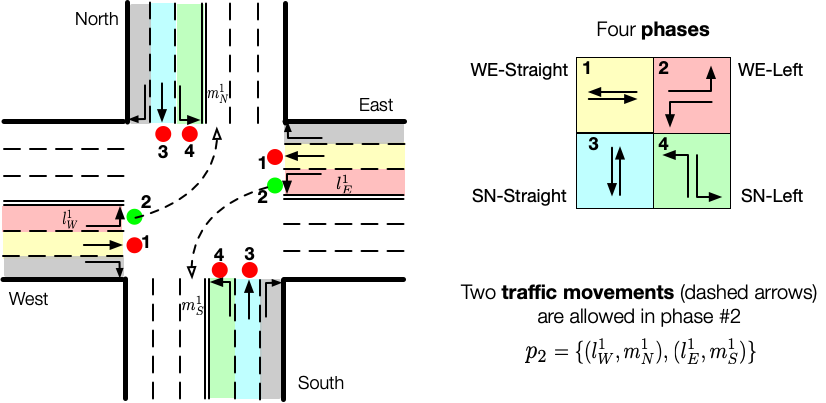
\includegraphics[width=0.8\textwidth]{figures/phase.png}
    \caption{Phase and traffic movements in traffic signal control problem. Phase \#2 is set in the example.}
    \label{fig:preliminary}
    % \vspace{-2mm}
\end{figure}

\vspace{-2mm}
% !TEX root = main.tex
\section{Method}

\subsection{Agent Design}
\label{sec:formulation}

First, we introduce the state, action and reward design for an agent that controls an intersection.
\begin{itemize}[wide,noitemsep,topsep=0pt]
    \item \textbf{State (Observation)}. Our state is defined for one intersection, which equals to the definition of observation in multi-agent RL. It includes the current phase $p$, the number of vehicles on each outgoing lane $x(m)$ ($m\in L_{out}$), and the number of vehicles on each segment of every incoming lane $x(l)_k$ ($l\in L_{in}$, $k=1\dots K$). In this chapter, each lane is evenly divided into 3 segments $(K=3)$, and we denote the segment on lane $l$ nearest to the intersection as the first segment $x(l)_1$.
    \item \textbf{Action}. At time $t$, each agent chooses a phase $p$ as its action $a_t$ from action set $\pmb{A}$, indicating the traffic signal should be set to phase $p$. In this chapter, each agent has four permissible actions, correspondingly four phases in Figure~\ref{fig:preliminary}. Each action candidate $a_{i}$ is represented as a one-hot vector. Note that in the real world the signal phases may organize in a cyclic way, while our action makes the traffic signal plan more flexible. Also, there may be different number of phases in the real world and four phases is not a must.
    \item \textbf{Reward}. We define the reward $r_i$ as
        \begin{equation}
            \label{eq:reward-detail}
            r_i  = - P_i,
        \end{equation}
    where $P_i$ is the  \textit{\textbf{pressure}} of intersection $i$, as defined in Equation~\eqref{eq:pressure}.
    
    Intuitively, the pressure $P_i$ indicates the degree of disequilibrium between vehicle density on the incoming and outgoing lanes. By minimizing $P_i$, the vehicles within the system can be evenly distributed. Then the green light is effectively utilized so that the throughput is optimized.
    
    % If we regard all the intersections have the same maximum capacity $x_{max}$ and $x(l,m)^{down}=\sum_{p\in Out_m}{r(m,p)\cdot x(m,p)}$ as the downstream number of vehicles and $x(l,m)$ as the incoming number of vehicles, then 
    % \begin{equation}
    % w(l,m)= x(l,m)-x^{down}(l,m)
    % \end{equation}
    % is simply \textit{the difference between the incoming and downstream number of vehicles}. If the vehicles are not allowed to change their lanes, then $|Out_m|=1$ and $r(m,p)=1$, we have $w(l,m)= x(l,m)-x(m,p)$, which is simply the difference of number of vehicles between the incoming and downstream lane.
\end{itemize}

\vspace{-1mm}
\subsection{Learning Process}

% At each time step $t$, each agent $i$ aim to find the action $a_i$ that lead to the maximum total discounted future reward:
% \begin{equation}
%     G^t_i=\Sigma_{k=t}^\infty\gamma^{k-t}r_i^t
% \end{equation}
% from time step $t$ onwards, where the discount factor $\gamma \in [0, 1]$ controls the importance of immediate rewards versus future rewards. 

% The policy $\pi$ of agent $i$ has a corresponding action-value function that gives the expected return conditioned on the observation $o$ and action $a$, when acting according to that policy:

% \begin{equation}
% Q^\pi_i(o,a) = \mathbb{E}[G^t_i|o_t=o,a_t=a,\pi]
% \end{equation}

% The optimal policy $\pi^*$ can be found by iteratively improving an estimate of the optimal action-value function
% \begin{equation}
% \label{eq:q_max}
% Q^*_i(o, a) := \max_\pi Q^\pi_i(o, a)
% \end{equation}
% using sample-based updates. Once $Q^*_i$
% is sufficiently approximated, acting greedy with respect to it yields the optimal policy.

% The Q-value function is estimated using a function approximator with weight vector $\theta: Q_i(o, a; \theta)$. 

In this chapter, we adopt Deep Q-Network (DQN) as function approximator to estimate the Q-value function. To stabilize the training process, we maintain an experience replay memory as described in~\cite{MKSR+15} by adding the new data samples in and removing the old samples occasionally. Periodically, the agent will take samples from the memory and use them to update the network.
% \begin{figure}[h!]
% \includegraphics[width = 250pt]{figures/qnetwork.png}
% \caption{Deep Q-network}
% \label{fig:q-network}
% \end{figure}


\section{Justification of RL agent}
To theoretically support the efficacy of our proposed method, we justify our reward and state design by showing that, in a simplified transportation system, the states we use can fully describe the system dynamics, and using Equation~\eqref{eq:reward-detail} as reward function in RL is equivalent to optimizing travel time as in the transportation methods. Some important notation is summarized in Table~\ref{tab:notations}.
\vspace{-3mm}

\begin{table}[htb]
\centering
  \caption{Summary of notation.}
  \label{tab:notations}
  \begin{tabular}{cl}
    \toprule
    Notation&Meaning\\
    \midrule
    $L_{in}$ & set of incoming lanes for an intersection \\
    $L_{out}$ & set of outgoing lanes for an intersection \\
	$(l,m)$ &\begin{tabular}[c]{@{}l@{}}a traffic movement from lane  $l$ to $m$
	\end{tabular} \\
    $x(l,m)$ & number of vehicles leaving $l$ and entering $m$\\
    $x(l)$ & number of vehicles on lane $l$\\
    $x(l)_k$ & number of vehicles on $k$-th segment of $l$\\
    $x_{max}(m)$ & maximum permissible vehicle number on lane $m$ \\
    $r(l,m)$ & turning ratio of traffic movements from $l$ to $m$\\
    $c(l,m)$ & discharging rate of movement $(l,m)$\\
    %$C(l,m)$ & saturation flow of phase $(l,m)$, vehicles per timestep\\
    $a(l,m)$ & \begin{tabular}[c]{@{}l@{}} 1 if the green light is on for movement $(l,m)$,\\ 0 otherwise
	\end{tabular} \\
	%$P_i$ & pressure on intersection $n$\\
    % $L$ & length of a road segment\\
  \bottomrule
\end{tabular}
\vspace{-3mm}
\end{table}

\subsection{Justification for State Design}

\subsubsection{General description of traffic movement process as a Markov chain}

Consider the arterial scenario described in Example~\ref{eg:inter}.
\begin{figure}[h!]
\centering
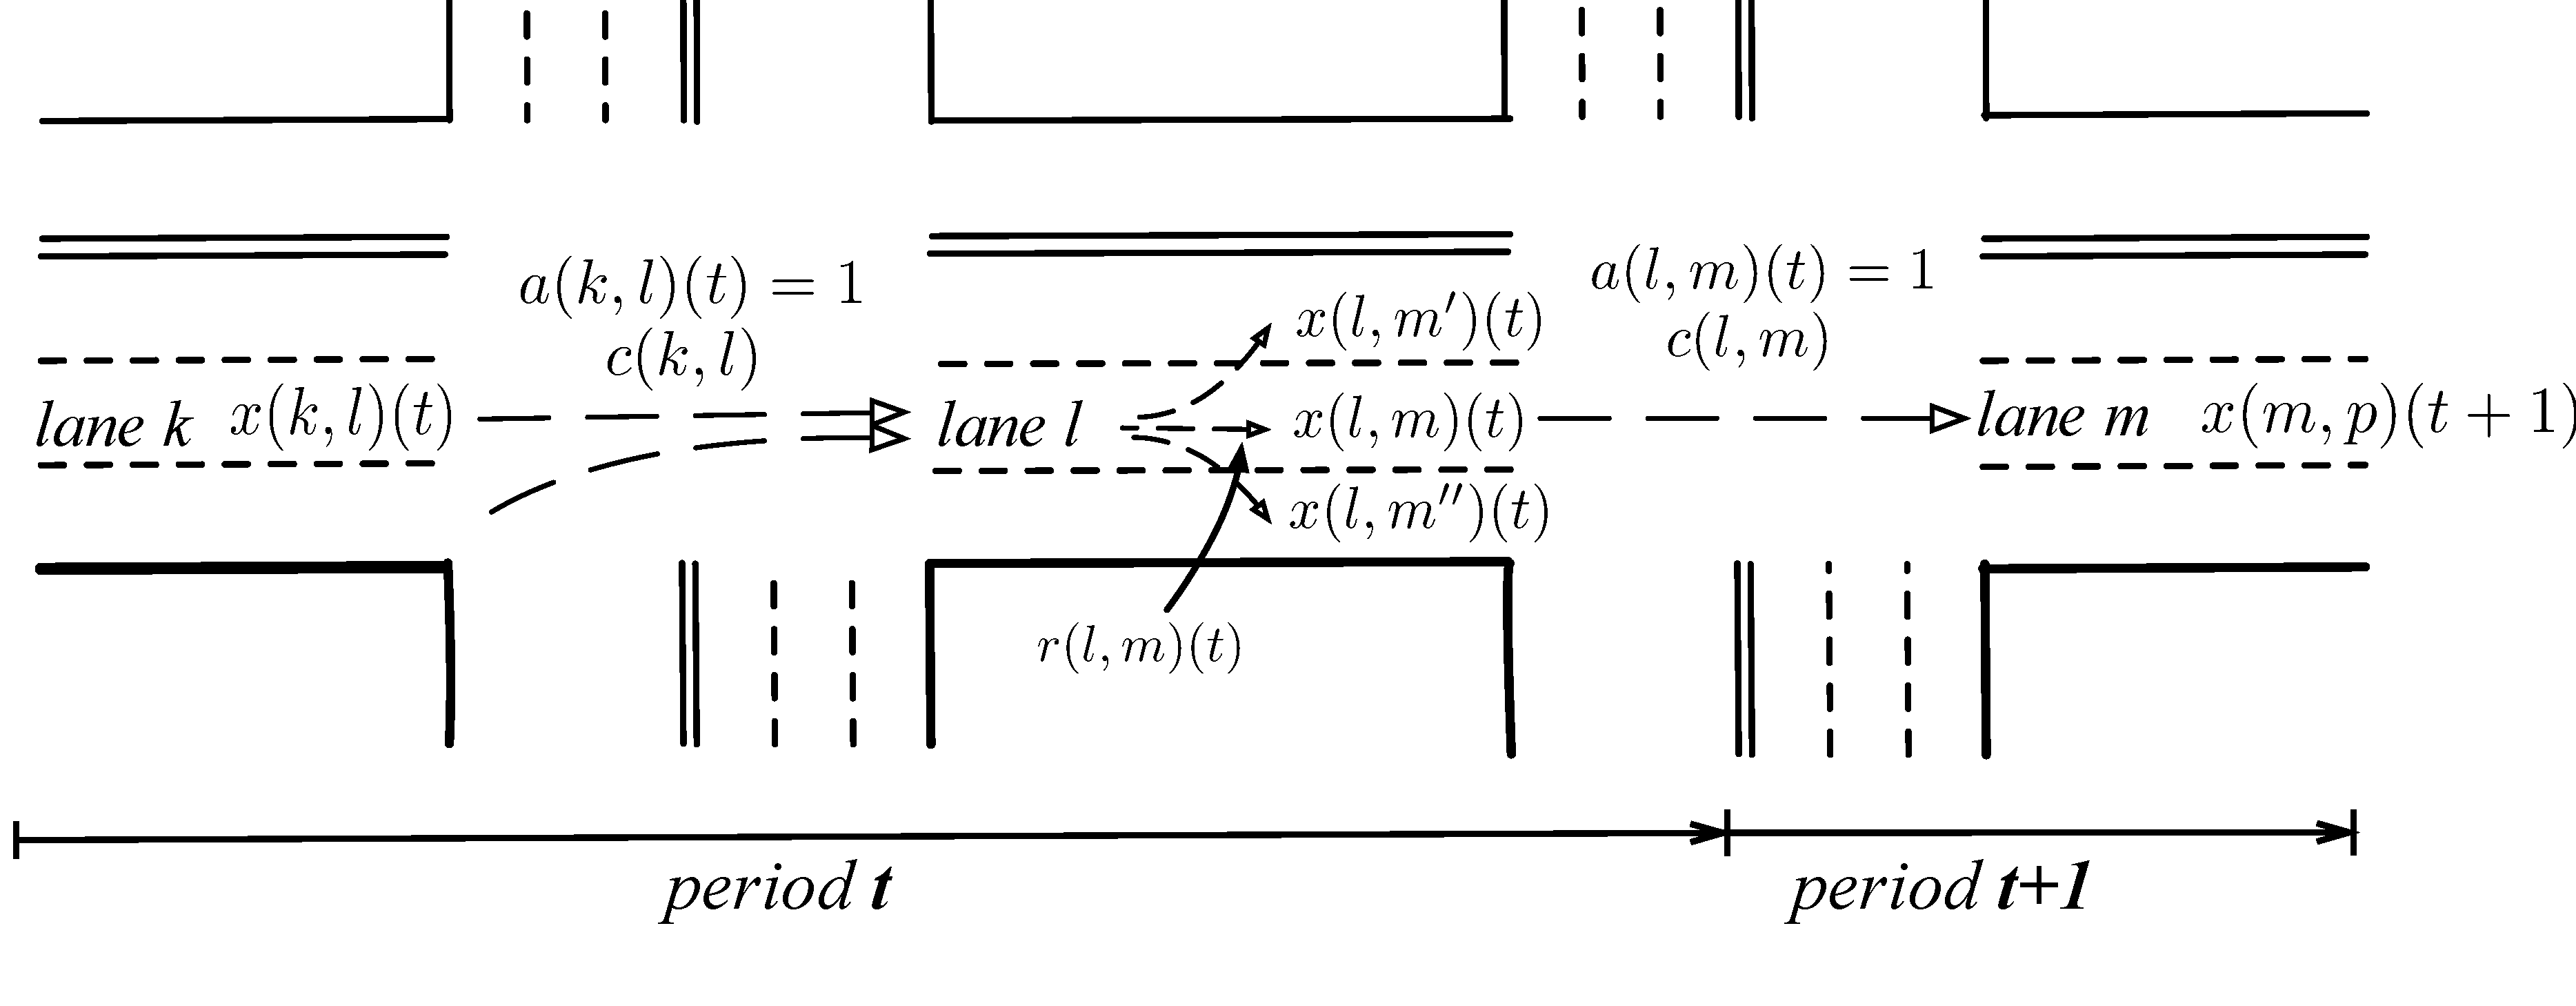
\includegraphics[width = 5.0in]{figures/SFM.pdf}
\caption{The transition of traffic movements.}
\label{fig:SFM}
\vspace{-3mm}
\end{figure}

\begin{example}
\label{eg:inter}
Figure~\ref{fig:SFM} associates a distinct traffic movement with each incoming lane $l\in L_{in}$ and each $m\in Out_l$, where $Out_l$ is the set of lanes output from lane $l$. 
Follow the notation from~\cite{MP13book}, let $x(l,m)(t)$ be the associated number of vehicles at beginning of period $t$, $X(t) = \{x(l,m)(t)\}$ is the $state$ of the movement network, which we regard as states $o^t$ in accordance with Section~\ref{sec:formulation}. There are two variables which are considered independent of $X(t)$: 
\begin{itemize}[wide,noitemsep,topsep=0pt]
    \item Turning ratio $r(l,m)$: $r(l,m)$ is an i.i.d. random variable indicating the proportion of vehicles entering $m$ from $l$ to the total vehicles on $l$. 
    
    \item Discharging rate $c(l,m)$: For each $(l,m)$, the queue discharging rate $c(l,m)$ is a non-negative, bounded, i.i.d. random variable,  i.e., $c(l,m)\leq C(l,m)$, where $C(l,m)$ is the saturation flow rate.
    
    % \item Demand $d(l,m)(t)$:  For each entry lane $l$, $d(l,m)$ are also non-negative bounded iid random variables. 
\end{itemize}

At the end of each period $t$, an action $A^t=\{(l,m)|a^t(l,m)\}$ must be selected from the action set $\pmb{A}^t$ as a function of $X^t$ for use in period $(t+1)$, indicating the agent will give green light for movements from $l$ to $m$, see the bottom of Figure~\ref{fig:SFM}. 

\end{example}

 The evolution equations of $X(t)$ are developed in~\cite{MP13}. For each $(l,m)$ and $t$, the evolution of $x(l,m)$ consists of receiving and discharging, and is captured by the following equation:
\begin{equation}
\begin{split}
\label{eq:queue-process}
      & x(l,m)(t+1) \\
    = &\ x(l,m)(t) + \ \underbrace{ \Sigma_{k\in In_l} min[c(k,l)\cdot a(k,l)(t),\ x(k,l)(t)]\cdot r(l,m)}_{receiving\ vehicles}\\
    - &\ \underbrace{ min\{c(l,m)\cdot a(l,m)(t),\ x(l,m)(t)\}\cdot \mathbf{1}(x(m)\le x_{max}(m))}_{discharging\ vehicles},\\
\end{split}
\end{equation}
where $In_l$ represents the set of lanes input to $l$. For the second term in Equation~\eqref{eq:queue-process}, when $l$ is the receiving lane, up to $x(k,l)$ vehicles will move from $k$ if $a(k,l)(t)=1$ and they will join $(l,m)$ if $r(l,m)=1$
For the third term in Equation~\eqref{eq:queue-process}, when traffic movement $(l,m)$ is actuated, i.e., $a(l,m)(t)=1$, up to $x(l,m)$ vehicles will leave $l$ and be routed to $m$ if there is no blockage on lane $m$, i.e., $x(m)\leq x_{max}(m)$, where $x_{max}(m)$ is the maximum permissible vehicle number on lane $m$. 

\nop{
    \begin{equation}
    x(l,m)(t+1) = x(l,m)(t)+\delta(l,m)(t)
    \end{equation}
    where,
    \begin{align*}
    g_l(t) = min\{c(l,m)(t+1)\cdot a(l,m)(t),\ x(l,m)(t)\}\cdot \mathbf{1}(x(m)\le x_{max}(m)), \\ l\in\mathcal{L}, m\in Out_l
    \end{align*}
    
    \begin{align*}
    f_l(t) = \sum_k min[c(k,l)(t+1)\cdot a(k,l)(t),\ x(k,l)]\cdot r(l,m)(t+1)\\
     l\in \mathcal{L}, k\in In_l\\
    \end{align*}
}

% For entry lanes of the system which have exogenous arrivals and no input lanes, the update equation is different: Equation~\ref{eq:queue-process} is modified to:
% \begin{equation}
% \begin{split}
% \label{eq:queue-process-entry}
%       & x(l,m)(t+1) \\
%     = & x(l,m)(t) +  d(l,m)(t)\\
%     - & min\{c(l,m)\cdot a(l,m)(t),\ x(l,m)(t)\}\cdot \mathbf{1}(x(m)\le x_{max}(m)) \\
% \end{split}
% \end{equation}

%In~\cite{MP13}, the time frame $t\rightarrow t+1$ is assumed to be the lane travel time, which has two disadvantages: (1) It assumes all the lane travel time is the same no matter the lane length. (2) It is resource consuming to take the traffic conditions $x(k,l)$ of nearby intersections. 

Suppose the initial state $X(1)={x(l,m)(1)}$ is a bounded random variable. Since $A(t)={a(l,m)(t)}$ is a function of the current state $X(t)$, and $c(l,m)$ and $r(l,m)$ are all independent of $X(1),...,X(t)$, the process $X(t)$ is a \textit{\textbf{Markov chain}}. The transition probabilities of the chain depend on the control policy.


\subsubsection{Specification with proposed state definition}
We can modify the traffic movement equation from lane-level to segment-level. We denote $x(l)_1$ as the number of vehicles on the segment $l_1$ closest to the intersection and $x(l)_2$ as the number of vehicles on the second closest segment, which is connected with $l_1$. Assume the vehicles change lanes for routing by the time it enters the lane $l$, i.e., $x(l,m)=x(l)$, and all vehicles on $l_{i+1}$ enter next segment $l_{i}$ during time $t$, then the movement process on the segment closest to the intersection can be written as:
\begin{equation}
\begin{split}
\label{eq:queue-process-segnment}
      & x(l)_1(t+1) = \ x(l)_1(t) + \ x(l)_2(t)\\
    - &\ min\{c(l,m)\cdot a(l,m)(t),\ x(l)_1(t)\}\cdot \mathbf{1}(x(m)\le x_{max}(m)). \\
\end{split}
\end{equation}
Equations for other segments can be derived in a similar way. 
 
With the lane and segment movement evolution equations described above, the evolution of an individual intersection could be obtained, which is a combination of the equations of all the lanes involved. For a single intersection $i$, $c(l,m)$ is a constant physical feature of each movement, whereas $x(l)_1$, $x(l)_2$, and $x(m)$ are provided to the RL agent in our state definition. Hence, our state definition can fully describe the dynamics of the system.


\subsection{Justification for Reward Design}
\subsubsection{Stabilization on traffic movements with proposed reward.}
Inspired by~\cite{MP13}, we first relax its assumption on physical queue expansion in the arterial. Then the goal of our RL agents is proven to stabilize the queue length, thus maximizes the system throughput and minimizes the travel time of vehicles.

%\theoremstyle{Definition}

\begin{definition}[Movement process stability] 
The movement process $X(t) = \{x(l, m)(t)\}$ is stable in the mean (and $u$ is a stabilizing control policy) if for
some $M<\infty$, the following holds:
\begin{equation}
\label{eq:stability}
    \sum_{t=1}^{T}\sum_{(l,m)}E[x(l,m)(t)]<M,\quad\forall T
\end{equation}
where $E$ denotes expectation. Movement stability in the mean implies that the chain is positive recurrent and has a unique steady-state probability distribution for all $T$. 
\end{definition}


\begin{definition}[Max-pressure control policy~\cite{MP13}] 
\label{def:maxpressure}
At each period $t$, the agent selects the action with maximum pressure at every state $X$: $
\tilde{A}^*(X) = \arg\max_{\tilde{A}\in \pmb{A}}\theta(\tilde{A}, X)$, where the pressure of $\tilde{A}$ is defined as
$$\theta(\tilde{A},X) = \sum_{(l,m):a(l,m)=1} \tilde{w}(l,m),$$
and $\tilde{w}(l,m) = x(l)- x(m)$ is the pressure of each movement. 
In this chapter, we use the tilde symbol for max-pressure policy, i.e., $\tilde{A}$, in order to differentiate it from a RL policy.
% \begin{equation}
% \label{eq:mp-pressure}
% \theta(\tilde{A},X) = \sum_{l,m:a(l,m)=1}c(l,m)\cdot \tilde{w}(l,m)(X)
% \end{equation}
\end{definition}

\begin{theorem}
\label{theo:stable} Without considering the physical queue expansion\footnote{``Without physical queue expansion'' means the vehicles will be considered to have no physical length in a queue.}, action $\tilde{A}^*$ selected by max-pressure control policy and action $A^*$ selected by our RL policy are both stabilizing the system, whenever the average demand is admissible\footnote{Intuitively, an admissible demand means the traffic demand can be accommodated by traffic signal control strategies, not including situations like long-lasting over-saturated traffic that requires perimeter control to stop traffic from getting in the system.}.
\end{theorem}

\begin{proof}For max-pressure control policy, Theorem 1 in~\cite{MP13} shows that given a time period $t=1,\ldots,T$ there exists $m<\infty$ and $\epsilon>0$ such that under $\tilde{A}^*$:
% \begin{equation}
% \label{eq:stability-proof}
% \epsilon\cdot\frac{1}{T}\sum_{t=1}^TE[X(t)]\leq m + \frac{1}{T}\cdot E[X(1)]^2
% \end{equation}
$\epsilon\cdot\frac{1}{T}\sum_{t=1}^TE[X(t)]\leq m + \frac{1}{T}\cdot E[X(1)]^2
$, 
where $X(1)$ denotes the state when $t=1$. 

For an optimal RL control policy, the agent selects the action $A$ with optimal $Q (A,X)$ at every state $X$:
\begin{equation}
\label{eq:q_max}
A^*(X) = \arg\max_{A\in \pmb{A}}Q(A, X).
\end{equation}
where $Q_t(A,X)= E[r_{t+1}+\gamma r_{t+2}+\dots | A, X]$ denotes the maximum total reward at state $X$ by taking $A$ at time $t$(in Equation~\eqref{eq:q_max}, we neglect time $t$ for simplicity).
The difference between the pressure definition in RL reward and max-pressure is that our RL agent uses the weighted pressure considering maximum permissible vehicle number $x_{max}$ in Equation~\eqref{eq:pressure-movement}. If we assume the lanes are in the same lenth $x_{max}(l)$, the stability result still holds for the normalized $x(l)$.
\end{proof}

\begin{theorem}
\label{theo:stable} Considering the physical queue expansion in the arterial environment, action $A^*$ selected by our RL policy is also stabilizing the movement.
\end{theorem}


\begin{figure*}[t!]
  \centering
    %   \begin{tabular}{ccc}
    %     %   \includegraphics[width=0.25\textwidth]{figures/case_beaver.png} &
    %     %   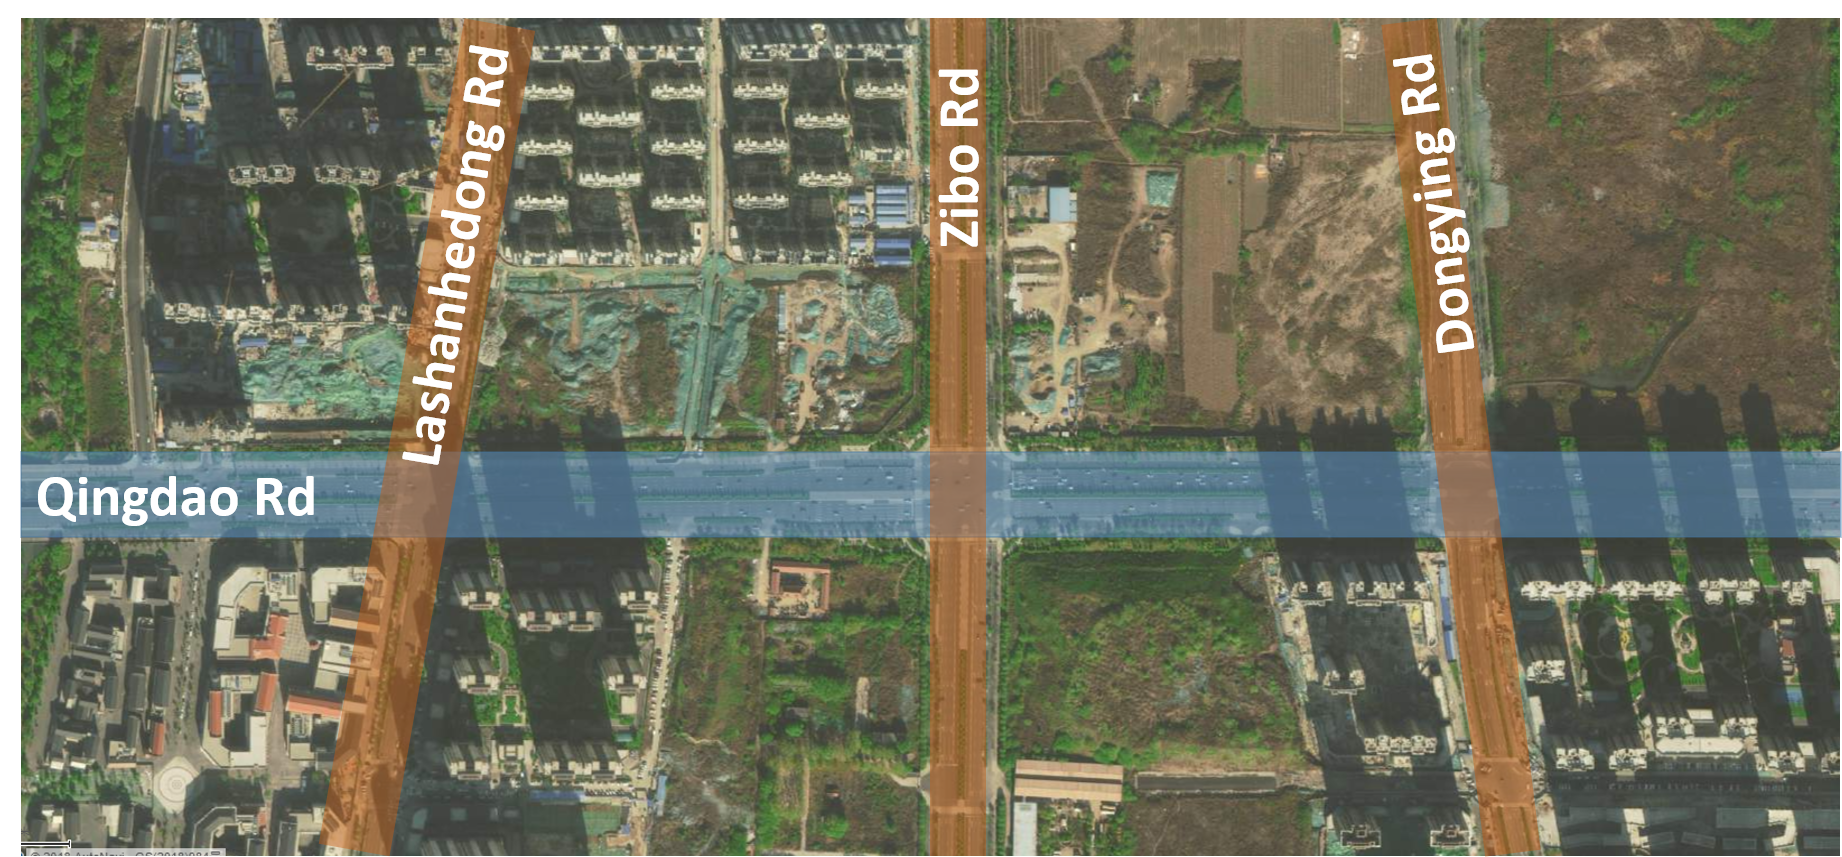
\includegraphics[width=0.22\textwidth]{figures/case_intersection_note.png}&
    %     %   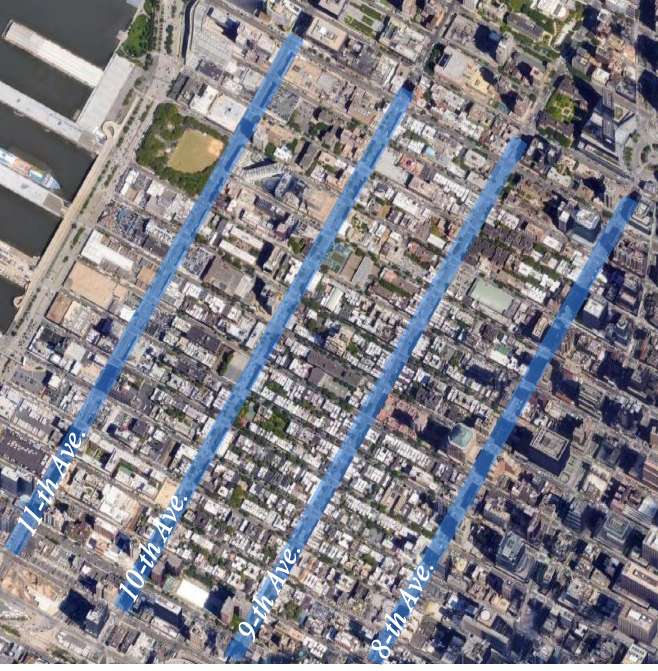
\includegraphics[width=0.42\textwidth]{figures/case_ny.png} \\
    %     %   \begin{tabular}[c]{@{}c@{}}(a) Beaver Avenue in State College, Pennsylvania, USA: \\a 5-intersection arterial with unidirectional traffic on the arterial\\ and bidirectional traffic on the side streets.\end{tabular}&
    %     %   \begin{tabular}[c]{@{}c@{}}(b) Qingdao Road in Jinan, China:\\ a 3-intersection arterial with bidirectional traffic \\on both the arterial and the side streets.\end{tabular}&
    %     %   \begin{tabular}[c]{@{}c@{}}(c) 8-th, 9-th, 10-th and 11-th Avenue in New York City, USA:\\ 16-intersection arterials with uni-directional traffic \\on both the arterial and the side streets.\end{tabular}\\
    %     %   \end{tabular}
    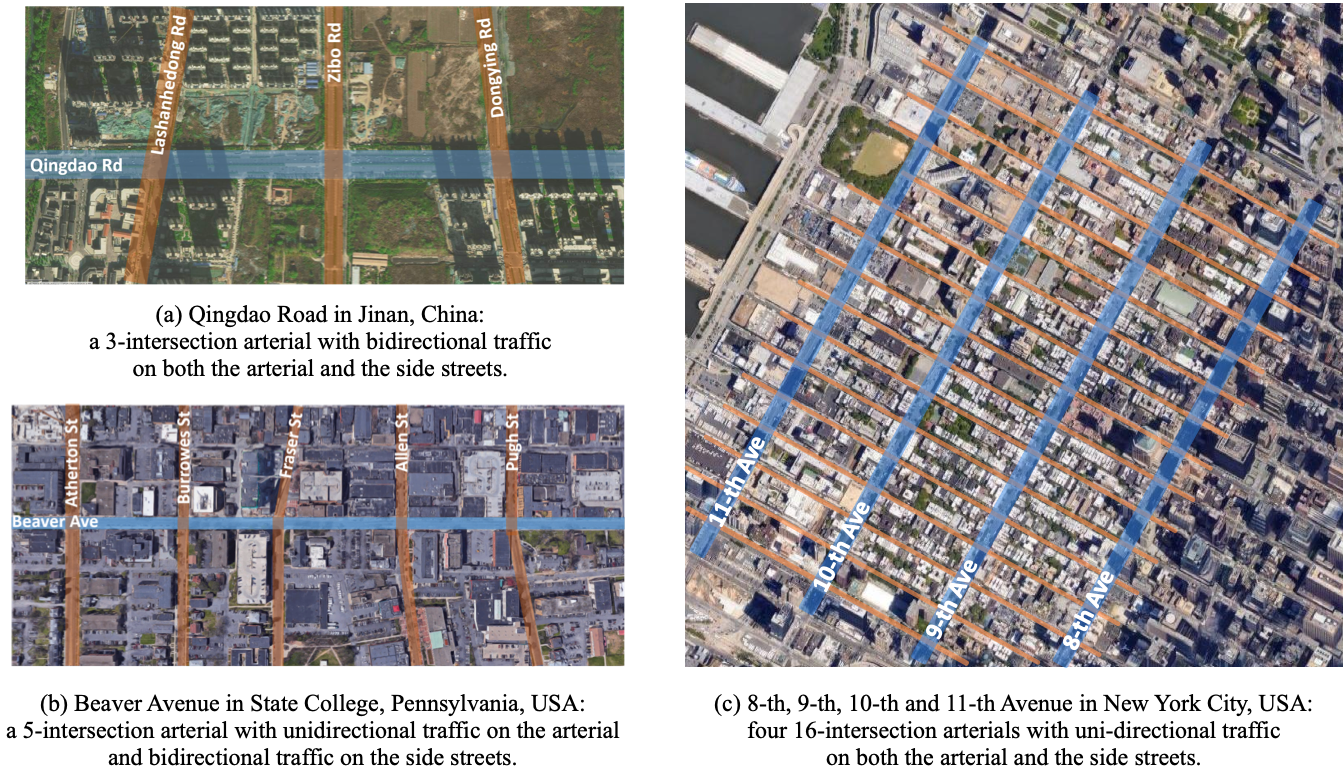
\includegraphics[width=1.0\textwidth]{figures/case_arterial.png}
     \caption{Real-world arterial network for the experiment.}
    \label{fig:real-intersection}
\end{figure*}

Different from~\cite{MP13}, we now establish the proof of Theorem~\ref{theo:stable}, which removes the assumption of no physical queue expansion in the arterial environment. In the arterial environment:
\begin{itemize}[wide,noitemsep,topsep=0pt]
    \item The maximum permissible vehicle number $x_{max}$ on side street lane $m^{side}$ is assumed to be infinite, hence the second term in Equation~\eqref{eq:pressure-movement} is zero. Thus we have $w(l,m^{side})=\frac{x(l)}{x_{max}(l)}>0$.
    \item When the outgoing lane $m^{main}$ along the arterial is saturated, the second term in Equation~\eqref{eq:pressure-movement} is approximately 1 because of the queue expansion. Thus $w(l,m^{main})\approx \frac{x(l)}{x_{max}(l)} -1 < 0$. 
\end{itemize}

This means when we consider the physical queue expansion in the arterial, $w(l,m^{side}) > w(l,m^{main})$, the control policy will restrict the queue spillback since it prohibits more vehicles to rush into the downstream intersection and block the movements of vehicles in other phases. Accordingly, $M$ in Equation~\eqref{eq:stability} can now be set to $M\leq \sum_{t=1}^{T}\sum_{(l,m)} x_{max}(m)$. 

\subsubsection{Connection to throughput maximization and travel time minimization.} Given that the traffic movement process of each intersection is stable, the system is accordingly stable. In an arterial environment without U-turn, vehicles that move from lane $m$ to $l$ would not move from $l$ to $m$ again, i.e.,  between $x(m,l)$ and $x(l,m)$ only one of them can exist under arterial network. Then the actions that RL agents take will not form gridlock or block the network, thus can efficiently utilize the green time. Within the given time period $T$, our RL agent can provide the maximum throughput, thus minimize the travel time of all vehicles within the system.

% !TEX root = main.tex

% \begin{figure*}[t!]
%   \centering
%   \begin{tabular}{cc}
%   \includegraphics[width=0.45\textwidth]{figures/case_beaver.png} &
%   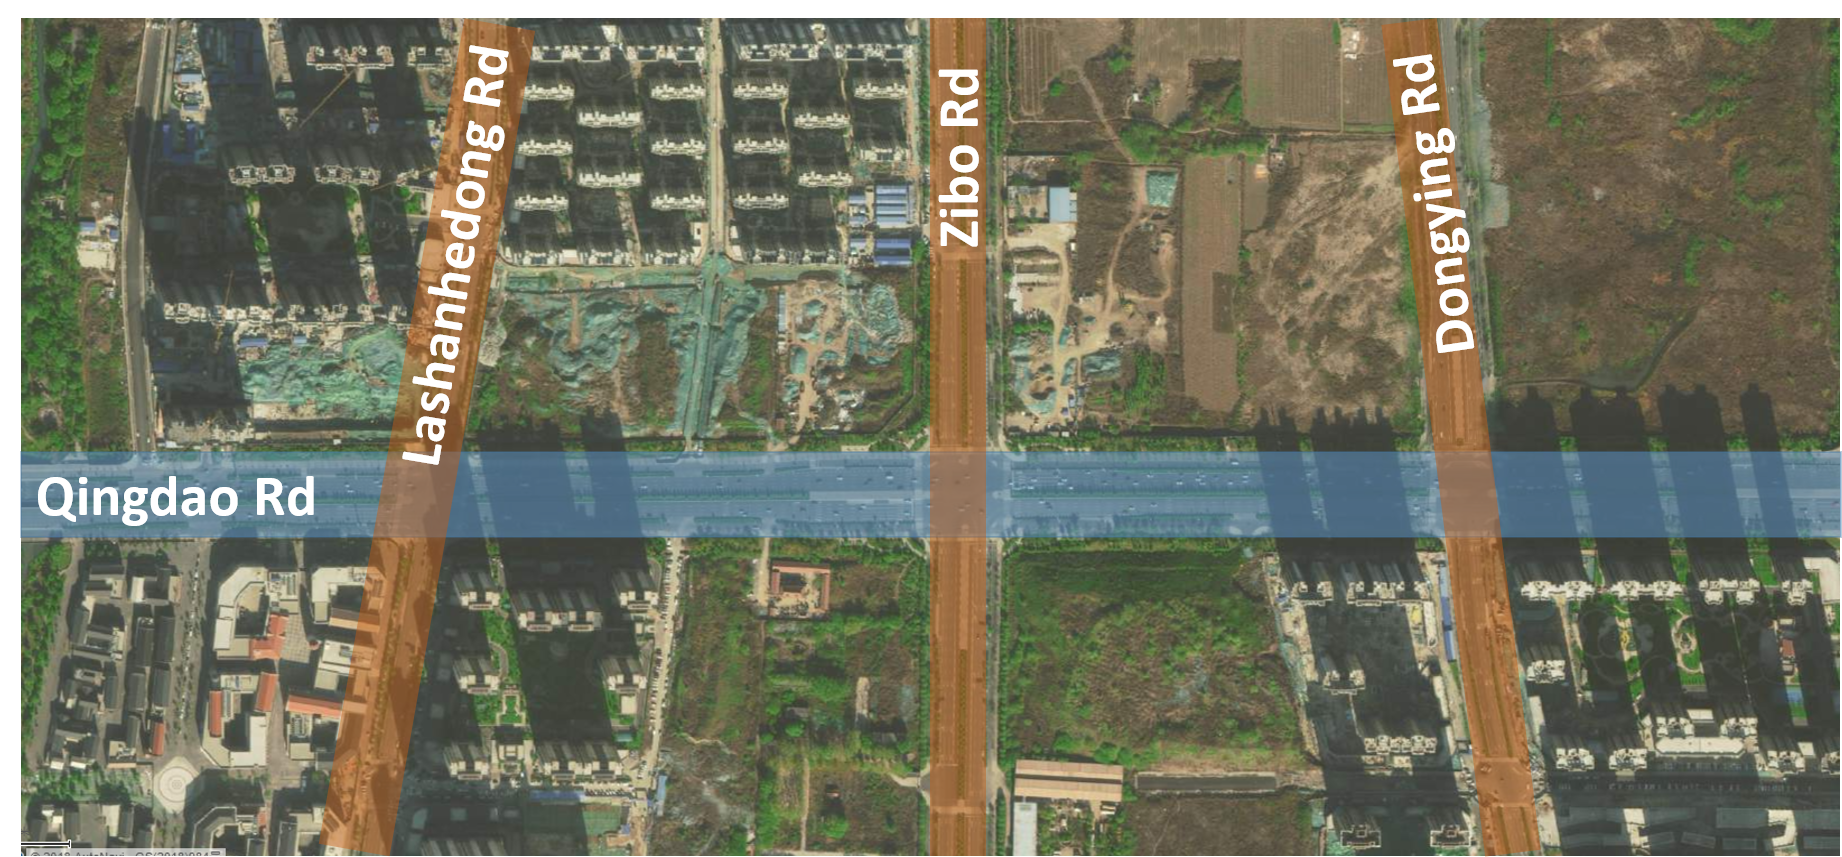
\includegraphics[width=0.42\textwidth]{figures/case_intersection_note.png} \\
%   \begin{tabular}[c]{@{}c@{}}(a) Beaver Avenue in State College, Pennsylvania, USA: \\a 5-intersection arterial with unidirectional traffic on the arterial\\ and bidirectional traffic on the side streets.\end{tabular}&
%   \begin{tabular}[c]{@{}c@{}}(b) Qingdao Road in Jinan, China:\\ a 3-intersection arterial with bidirectional traffic \\on both the arterial and the side streets.\end{tabular}\\
%   \end{tabular}
   
%      \caption{Real-world arterials for experiment.}
%     \label{fig:real-intersection}
% \end{figure*}

\section{Experiment}
We conduct experiments on CityFlow\footnote{http://cityflow-project.github.io}, an open-source traffic simulator that supports large-scale traffic signal control~\cite{huichu19}. After the traffic data being fed into the simulator, a vehicle moves towards its destination according to the setting of the environment. The simulator provides the state to the signal control method and executes the traffic signal actions from the control method.\footnote{Codes, public datasets and their preprocessing and
statistical details can be found at: https://github.com/wingsweihua/presslight. \\More datasets can be found at: http://traffic-signal-control.github.io}

\subsection{Dataset Description}
Both synthetic and real-world traffic flow data are used in our experiments. In a traffic dataset, each vehicle is described as $(o, t, d)$, where $o$ is  origin location, $t$ is  time, and $d$ is  destination location. Locations $o$ and $d$ are both locations on the road network. Traffic data is taken as input for the simulator. All the data contains bi-directional and dynamic flows with turning traffic. 

% \subsubsection{Road network data}
% Without losing generality, following road networks are tested in our experiment:
% \begin{itemize}[wide,noitemsep,topsep=0pt]
% \item Arterials with different numbers (6, 10, 20) of homogeneous intersections. 
% %, see Figure~\ref{fig:Traffic-direc-pattern}. 
% Each lane is five meters wide and 300 meters long. We use this environment to show the effectiveness of our method under different kinds of traffic flows. 
% % \begin{figure}[htb]
% %   \centering
% % 	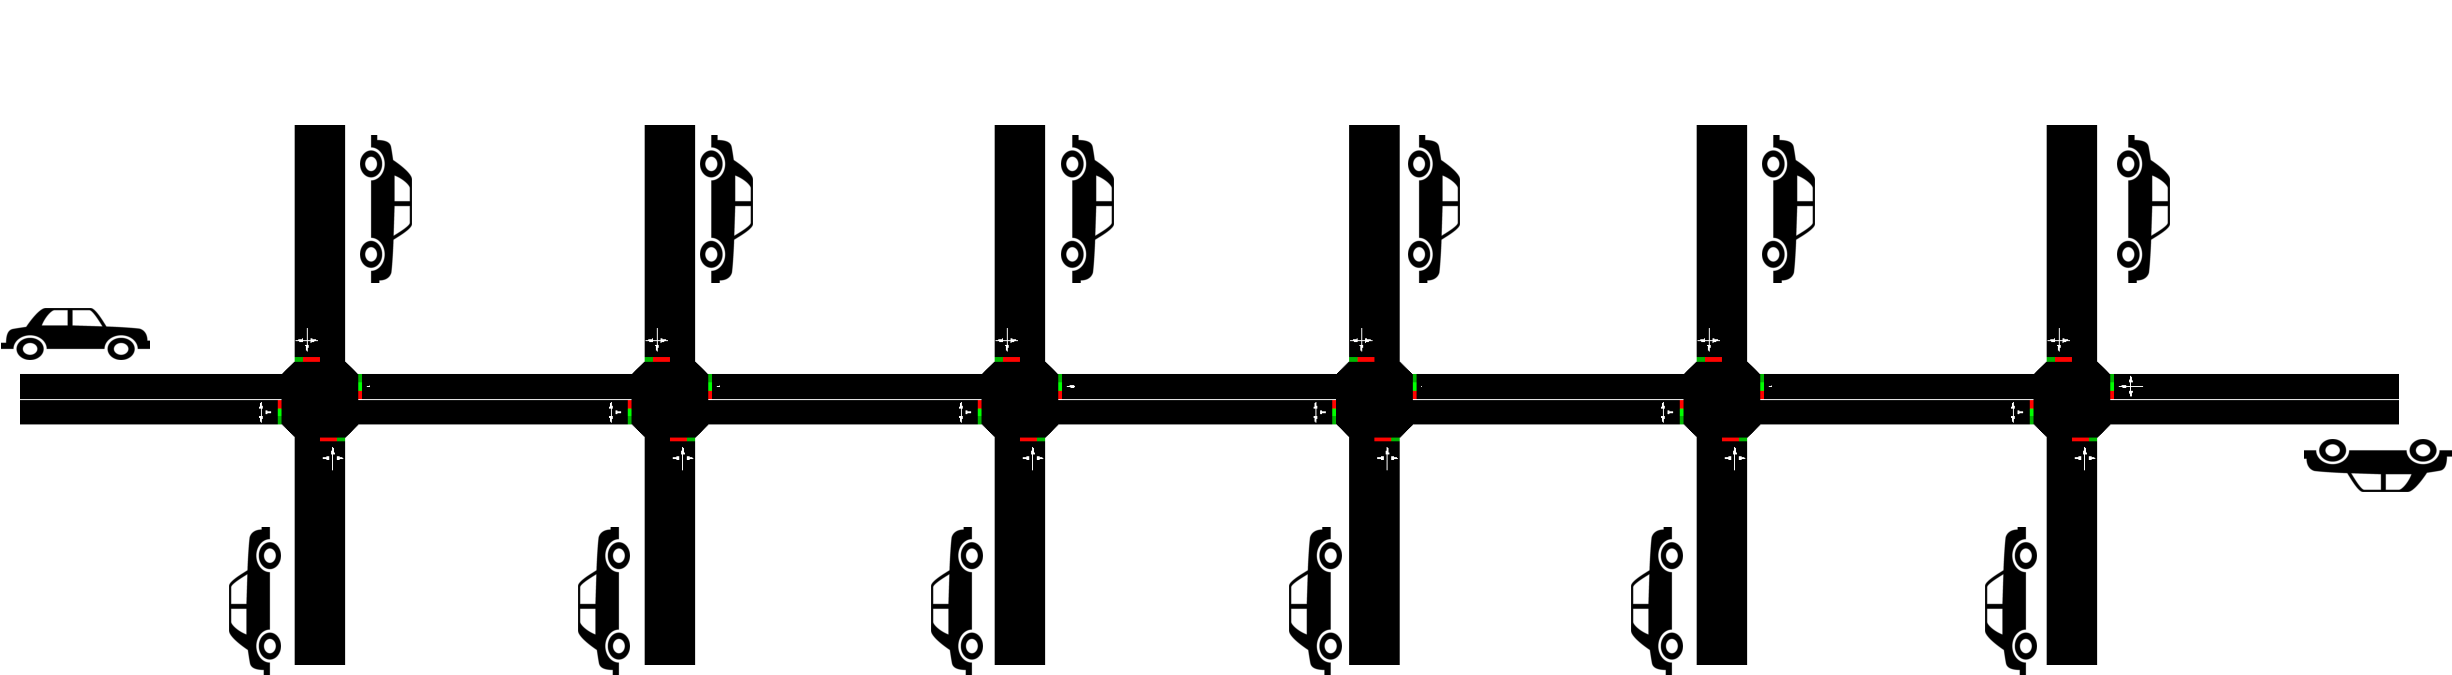
\includegraphics[width=0.48\textwidth]{figures/arterial_6.pdf}
% %      \caption{Bidirectional traffic on an arterial with 6 intersections.}   
% %     \label{fig:Traffic-direc-pattern}
% % \end{figure}
% % \item Arterial with 6 homogeneous intersections. This part of experiments are conducted on an arterial with four-leg intersections, see Figure~\ref{fig:Traffic-direc-pattern}. Each lane is 5 meters wide and 300 meters long. We use this environment to show the effectiveness of our method under different kinds of traffic flows. 
% \item Three-intersection arterials with different length of lanes (300-meters long and 150-meters long), and different legs (3 legs and 4 legs), as illustrated in~\ref{fig:heter_inter}. We use these road networks to show the capability of our model dealing with heterogeneous intersections.
% \item A $3\times3$ grid network with nine homogeneous intersections. This part of experiments are conducted to show the scalability of our methods.
% \item A real-world arterial in State College, Pennsylvania. This is an arterial with five intersections, each of which is a 4-leg intersection with 100 meters of both incoming and downstream sides. The arterial is one-way with two lanes, while the side streets have bi-directional traffic with one lane for each direction. Its arterial image is shown in~\ref{fig:real-intersection}(a).
% \item A real-world arterial in Jinan, China. The arterial has three 4-leg intersections with 300 meters of both incoming and downstream. Each intersection have the same structure as aforementioned homogeneous arterial. Its aerial image is shown in~\ref{fig:real-intersection}(b).
% \end{itemize}
%\subsubsection{Traffic flow data}

\begin{itemize}[wide,noitemsep,topsep=0pt]
\item {\bf Synthetic data}. Four different configurations are tested as detailed in Table~\ref{tab:synthetic-table}. This data is synthesized from a statistical analysis of real-world traffic patterns in Jinan and Hangzhou. 
\item {\bf Real-world data}. We collect six representative traffic flow data from three cities to evaluate the performance of our model: Beaver Avenue in State College, USA; Qingdao Road in Jinan, China; four avenues in Manhattan, New York City, USA. Figure~\ref{fig:real-intersection} shows the aerial view on these arterials. Detailed statistics of these datasets are listed in Table~\ref{tab:real-table}. 
\end{itemize}

\subsection{Experimental Settings}

\subsubsection{Environmental settings}
Different road networks are configured. Besides a six-intersection arterial on which we primarily experiment, arterials with larger scale and heterogeneous intersections (in Figure~\ref{fig:heter_inter}) are also tested. 

The free-flow speed on the road segments is set to 40 kilometers/hour. Vehicles can always turn right when there is no conflicting traffic. Every time the phase switches, a 5-second combined yellow and all-red time are followed to clear the intersection. 
%Note that phase (3) and phase (4){\color{blue}consistent notation} would be disabled when there is no turning traffic.

\begin{table}[h!]
\begin{center}
% \vspace{-2mm}
\caption{Configurations for synthetic traffic data}
\label{tab:synthetic-table}
\begin{tabular}{lccc}
\toprule
Config        & \begin{tabular}[c]{@{}c@{}}Demand \\ pattern \end{tabular}  & \begin{tabular}[c]{@{}c@{}}Arrival rate\\ (vehicles/h/road)\end{tabular}  &  Volume      \\ \midrule
1. Light-Flat & Flat           & \multirow{2}{*}{\begin{tabular}[c]{@{}c@{}}Arterial : 600\\ Side-street: 180\end{tabular}}  &\multirow{2}{*}{\begin{tabular}[c]{@{}c@{}} (Light) \end{tabular}} \\ \cline{1-2}
2. Light-Peak & Peak           &                                                                                             & \\ \bottomrule
3. Heavy-Flat & Flat           & \multirow{2}{*}{\begin{tabular}[c]{@{}c@{}}Arterial: 1400\\ Side-street : 420 \end{tabular}}  &    \multirow{2}{*}{\begin{tabular}[c]{@{}c@{}} (Heavy) \end{tabular}}  \\ \cline{1-2}
4. Heavy-Peak & Peak           &                                                                                               &  \\ \hline
\end{tabular}
% \vspace{-2mm}
\end{center}
\end{table}

\begin{table}[t]
\begin{center}
\caption{Data statistics of real-world traffic dataset}
\label{tab:real-table}
\begin{tabular}{cccccc}
\toprule
\multirow{2}{*}{Dataset}  & \multicolumn{4}{c}{Arrival rate (vehicles/h)}  & \multirow{2}{*}{\begin{tabular}[c]{@{}c@{}}\# of inter- \\ sections\end{tabular}}\\
                           & Mean         & Std         & Max       & Min    &    \\\midrule
\begin{tabular}[c]{@{}c@{}}Qingdao Rd., Jinan \end{tabular} & 3338.83       & 221.58       & 2748       & 3864   & 3   \\
\begin{tabular}[c]{@{}c@{}}Beaver Ave., \\ State College \end{tabular}      & 2982.33       & 359.70       & 2724       & 3491   & 5    \\
8-th Ave., NYC      & 6790.04       & 32.34  &  4968      &  7536   & 16   \\
9-th Ave., NYC      & 4513.06       & 25.88       & 4416       & 6708    & 16   \\
10-th Ave., NYC    & 6083.90       & 25.61       & 2892       & 5016     & 16   \\
11-th Ave., NYC     & 4030.79       & 24.08       & 2472       & 4536    & 16    \\
\bottomrule
\end{tabular}
% \vspace{-2mm}
\end{center}
\end{table}

\subsubsection{Evaluation metric}
Following existing studies~\cite{wei2018intellilight}, we use the average \textbf{travel time} in seconds to evaluate the performance. The average travel time of all vehicles is the most frequently used measure in the transportation field~\cite{Roess2011t}, which is calculated as the average travel time of all vehicles spent in the system.

\subsubsection{Compared methods}
We compare our model with the following two categories of methods: transportation methods and RL methods. Note that all methods are carefully tuned and their best results are reported (except the offsets of $\FT$ because of its random nature).
% Also, for fair comparison, all RL models are learnt from scratch without any pre-trained parameters.

\textit{Conventional transportation baselines:}
\begin{itemize}[wide,noitemsep,topsep=0pt]

\item \textbf{\FT}: Fixed-time with random offset~\cite{Roess2011t}. Each phase has a fixed time of 15 seconds. For uni-directional traffic, there are only 2 phases (WE-straight, SN-straight). For traffic with turning vehicles, there are 4 phases. 


\item \textbf{\Greenwave}~\cite{Roess2011t}:  This is the most classical method in transportation field to implement coordination that gives an optimal solution for unidirectional and uniform traffic on the arterial. It requires that all intersections share the same cycle length, which is the minimum value of the cycle length for individual intersections calculated using Webster's theory~\cite{Webst58}. The phase split percentage equals to the percentage between the demand of a designated phase and total demand. Offsets between intersections are equivalent to the free-flow travel time between two consecutive intersections. 

\item \textbf{\Maxpressure}: Max pressure control~\cite{varaiya2013max} is a state-of-the-art network-level traffic signal control method, which greedily chooses the phase with the maximum pressure, as introduced in Definition~\ref{def:maxpressure}.

\end{itemize}

\textit{RL baselines:}
\begin{itemize}[wide,noitemsep,topsep=0pt]
\item \textbf{\LIT} is an individual deep reinforcement learning approach proposed in \cite{ZZXW+19}. This method does not consider the traffic condition on downstream lanes in state and uses a reward with queue length. 

\item \textbf{\NIPS} is a coordinated reinforcement learning approach for multi-intersection control~\cite{VaOl16}. Specifically, the coordination is to design a coordination graph and to learn the joint local Q-function on two adjacent intersections directly.
\end{itemize}

\begin{table*}[tp!]
\caption{Performance comparison on synthetic data between all the methods in the arterial with 6 intersections w.r.t. average travel time (the lower the better). Top-down: conventional transportation methods, learning methods, and our proposed method. }
\label{tab:RQ1-result}
\centering
\begin{tabular}{p{0.2\textwidth}p{0.1\textwidth}p{0.1\textwidth}p{0.1\textwidth}p{0.1\textwidth}}
\toprule
& \multicolumn{4}{c}{Synthetic traffic }  \\ 
& LightFlat & LightPeak  & HeavyFlat& HeavyPeak \\ \midrule
\FT             &\multicolumn{1}{c}{  93.29   		}&\multicolumn{1}{c}{   109.50        }&\multicolumn{1}{c}{    325.48       }&\multicolumn{1}{c}{   246.25         } \\ 
\Greenwave      &\multicolumn{1}{c}{  98.39    	}&\multicolumn{1}{c}{  124.09         }&\multicolumn{1}{c}{   263.36        }&\multicolumn{1}{c}{   286.85         }\\

\Maxpressure    &\multicolumn{1}{c}{  74.30       	}&\multicolumn{1}{c}{  82.37          }&\multicolumn{1}{c}{   262.26        }&\multicolumn{1}{c}{   225.60         }\\
 \midrule
\NIPS           &\multicolumn{1}{c}{ 123.02   	}&\multicolumn{1}{c}{  115.85      }&\multicolumn{1}{c}{  525.64         }&\multicolumn{1}{c}{  757.73          }\\ 
\LIT      &\multicolumn{1}{c}{  65.07       	}&\multicolumn{1}{c}{  66.77      	  }&\multicolumn{1}{c}{   233.17        }&\multicolumn{1}{c}{   258.33         }\\
 \midrule
\textbf{\PressLight}     &\multicolumn{1}{c}{\textbf{59.96}}	&\multicolumn{1}{c}{  \textbf{61.34}} &\multicolumn{1}{c}{ \textbf{160.48} }&\multicolumn{1}{c}{  \textbf{184.51} }\\ 

\bottomrule
\end{tabular}
\end{table*}

\begin{table*}[tp!]
\caption{Performance comparison on real-world data between all the methods in the arterial with 6 intersections w.r.t. average travel time (the lower the better). Top-down: conventional transportation methods, learning methods, and our proposed method. }
\label{tab:RQ1-result-2}
\centering
\begin{tabular}{p{0.1\textwidth}p{0.1\textwidth}p{0.1\textwidth}p{0.1\textwidth}p{0.1\textwidth}p{0.1\textwidth}p{0.1\textwidth}}
\toprule
& \multicolumn{6}{c}{Real-world traffic}  \\ 
& \begin{tabular}[c]{@{}c@{}}Qingdao Rd.,\\ Jinan\end{tabular} & \begin{tabular}[c]{@{}c@{}}Beaver Ave.,\\ State College\end{tabular}& \begin{tabular}[c]{@{}c@{}}8th Ave.,\\ NYC\end{tabular} &\begin{tabular}[c]{@{}c@{}}9th Ave.,\\ NYC\end{tabular}&\begin{tabular}[c]{@{}c@{}}10th Ave.,\\ NYC\end{tabular}&\begin{tabular}[c]{@{}c@{}}11th Ave.,\\ NYC\end{tabular}  \\ \midrule
\FT             &\multicolumn{1}{c}{  317.40         }&\multicolumn{1}{c}{    336.29                   	}&\multicolumn{1}{c}{ 432.60  }&\multicolumn{1}{c}{	469.54}&\multicolumn{1}{c}{347.05   	}   &\multicolumn{1}{c}{  368.84} \\ 
\Greenwave      &\multicolumn{1}{c}{   370.30        }&\multicolumn{1}{c}{   332.06                		}&\multicolumn{1}{c}{ 451.98  }&\multicolumn{1}{c}{	502.30}&\multicolumn{1}{c}{317.02   	}&\multicolumn{1}{c}{  314.08}\\ 
\Maxpressure    &\multicolumn{1}{c}{ 567.06          }&\multicolumn{1}{c}{     222.90               	 	}&\multicolumn{1}{c}{ 412.58  }&\multicolumn{1}{c}{	370.61}&\multicolumn{1}{c}{392.77   	}&\multicolumn{1}{c}{  224.54}\\ \midrule
\NIPS          &\multicolumn{1}{c}{ 238.19        }&\multicolumn{1}{c}{  455.42        	  		 	}&\multicolumn{1}{c}{704.98}&\multicolumn{1}{c}{669.69			  }&\multicolumn{1}{c}{676.19	}&\multicolumn{1}{c}{548.34}\\ 
\LIT      &\multicolumn{1}{c}{     58.18       }&\multicolumn{1}{c}{    338.52   		  		 	}&\multicolumn{1}{c}{ 471.30  }&\multicolumn{1}{c}{	726.04}&\multicolumn{1}{c}{309.95   	}&\multicolumn{1}{c}{  340.40}\\ \midrule
\textbf{\PressLight}     &\multicolumn{1}{c}{ \textbf{54.87}   }&\multicolumn{1}{c}{  \textbf{92.00}        		}&\multicolumn{1}{c}{ \textbf{223.36 }} &\multicolumn{1}{c}{	\textbf{149.01}}&\multicolumn{1}{c}{\textbf{161.21	} 	}&\multicolumn{1}{c}{  \textbf{140.82}}\\ 
% Improvements &   7.85\%          &  8.13\%           &       5.69\%         &      31.17\%       &   28.58\%          &    58.73\%             \\ 
\bottomrule
\end{tabular}
\end{table*}

\subsection{Performance Comparison}
Table~\ref{tab:RQ1-result} reports our experimental results using synthetic data under six-intersection arterial and real-world data \textit{w.r.t.} average travel time. 
We have the following findings:

(1) Conventional transportation methods (\FT, \Greenwave and \Maxpressure) give poor performance. This is because the traffic in these settings is dynamic. Conventional methods, which rely heavily on over-simplified assumptions or prior knowledge on the traffic, may easily fail under the dynamic traffic scenarios.

(2) Our method \PressLight outperforms all other RL methods. Though all the methods aim to learn to minimize the travel time, our reward design is proven to directly optimize towards it, while \NIPS and \LIT are using mixed reward which may distract the model from learning efficiently.

(3) When the traffic grows larger (Config 3,4 to 1,2), \PressLight becomes much better than other baselines. Under heavy traffic, a poor control strategy would make downstream queue may easily spill back and the green time would be wasted. The reward design of our agents considers balancing the queues on all the intersections within the arterial, which makes the performance even superior as the traffic becomes larger. 
    

%Learning based methods performs better than conventional transportation methods. It makes sense since the RL methods does not require much prior knowledge and can learn to adjust the control policy.

\subsection{Study of \PressLight}

\paragraph{Effects of variants of our proposed method} We consider several variations of our model as follows.

\begin{table}[t!]
\centering
\caption{Detailed comparison of our proposed state and reward design and their effects w.r.t. average travel time (lower the better) under synthetic traffic data.}
\label{tab:variants-result}
% \centering
\begin{tabular}{ccccc}
\toprule
           & \HeavyFlat & \HeavyPeak \\ \midrule
\base        & 233.17      &  258.33       \\ 
\NDeeplight      & 201.56      &  281.21     \\ 
\SNDeeplight    & 200.28      &  196.34     \\ 
\textbf{\PressLight} & \textbf{160.48} &  \textbf{184.51}     \\ \bottomrule
\end{tabular}
% \vspace{-3mm}
\end{table}

\begin{itemize}[wide,noitemsep,topsep=0pt]
    \item \textbf{\base}. Instead of using the distribution of the vehicles, \base simply uses phase and number of vehicles on each incoming lanes as its state (similar to \LIT), and uses the reward defined same as \LIT. This serves as a base model for later variants.
    %\item \textbf{\SDeeplight}: By adding coming vehicle distribution (the number of vehicles on each segment of lanes) to the state of \base, which is more delicate state design, the agents will have more information about its incoming intersections than \base agents.
    \item \textbf{\NDeeplight}. Based on \base, \NDeeplight adds the number of vehicles on outgoing lanes to its state, which has more information about its downstream intersections than \base agents.
    \item \textbf{\SNDeeplight}. Based on \NDeeplight, \SNDeeplight uses the phase, the number of segments' vehicles on both incoming and outgoing lanes into its state, which is the same as our proposed state definition.
    \item \textbf{\PressLight}. Our proposed method which further changes \SNDeeplight's reward to pressure.
\end{itemize}

Table~\ref{tab:variants-result} shows the performance of variants of our method:
\begin{enumerate}[wide,noitemsep,topsep=0pt]
    %\item By adding incoming vehicle distribution information, \SDeeplight outperforms \base in all settings. This is because compared with \base's state as number of vehicles, \SDeeplight is able to observe the distribution of coming vehicles and decide when to change the light for them to optimize the offsets between intersections.  optimizing queue length of each agents individually would ignore the congestion on neighboring intersections. Hence, inspired by \Maxpressure, the reward is modified from minimizing queue length to minimizing the difference of queue lengths of all the incoming lanes and queue lengths of outgoing lanes. 
    % \item Adding vehicle information on outgoing lanes boosts the performance of \base. This makes sense since \NDeeplight is able to observe traffic condition on outgoing lanes and helps balancing the queues for each intersection when there is congestion on downstream lanes.
    % \item By adding incoming vehicle distribution, \SNDeeplight outperforms \NDeeplight in both settings. One reason could be that compared with \base's state as number of vehicles, \SDeeplight is able to observe the distribution of coming vehicles and decide when to change the light for them to optimize the offsets between intersections. This shows that the effectiveness of our state design.
    \item Giving the added state information (\NDeeplight and \SNDeeplight) boosts the performance. This makes sense since (1) \NDeeplight is able to observe traffic condition on outgoing lanes and helps to balance the queues for each intersection when there is congestion on outgoing lanes; (2) \SNDeeplight has the information about vehicle distributions which is the key factor for agents to learn the offsets.
    \item \PressLight further outperforms \SNDeeplight owing to its reward definition. Instead of optimizing a reward that is not directly towards the travel time under arterial network, our reward design is proved to be a surrogate of average travel time. This demonstrates the effectiveness of our proposed reward design.  
\end{enumerate}

% \begin{table}[tbh]
% \caption{Performance on heterogeneous network for config.3 on an arterial with 3 intersections }
% \label{tab:hete-result}
% \begin{tabular}{ccccc}
% \toprule
%           & 3 leg &  different length \\ \midrule
% MP        & 156.76      &  200.51     \\ 
% PressLight & 111.46     &  134.44     \\ \bottomrule
% \end{tabular}
% \end{table}

\paragraph{Average travel time related to pressure.}
Figure~\ref{fig:convergence} illustrates the convergence curve of our agents learning process w.r.t. the average reward and the average pressure of each round. We can see that the travel time is closely correlated with pressure.

\begin{figure}[t]
\begin{center}
  \begin{tabular}{c}
   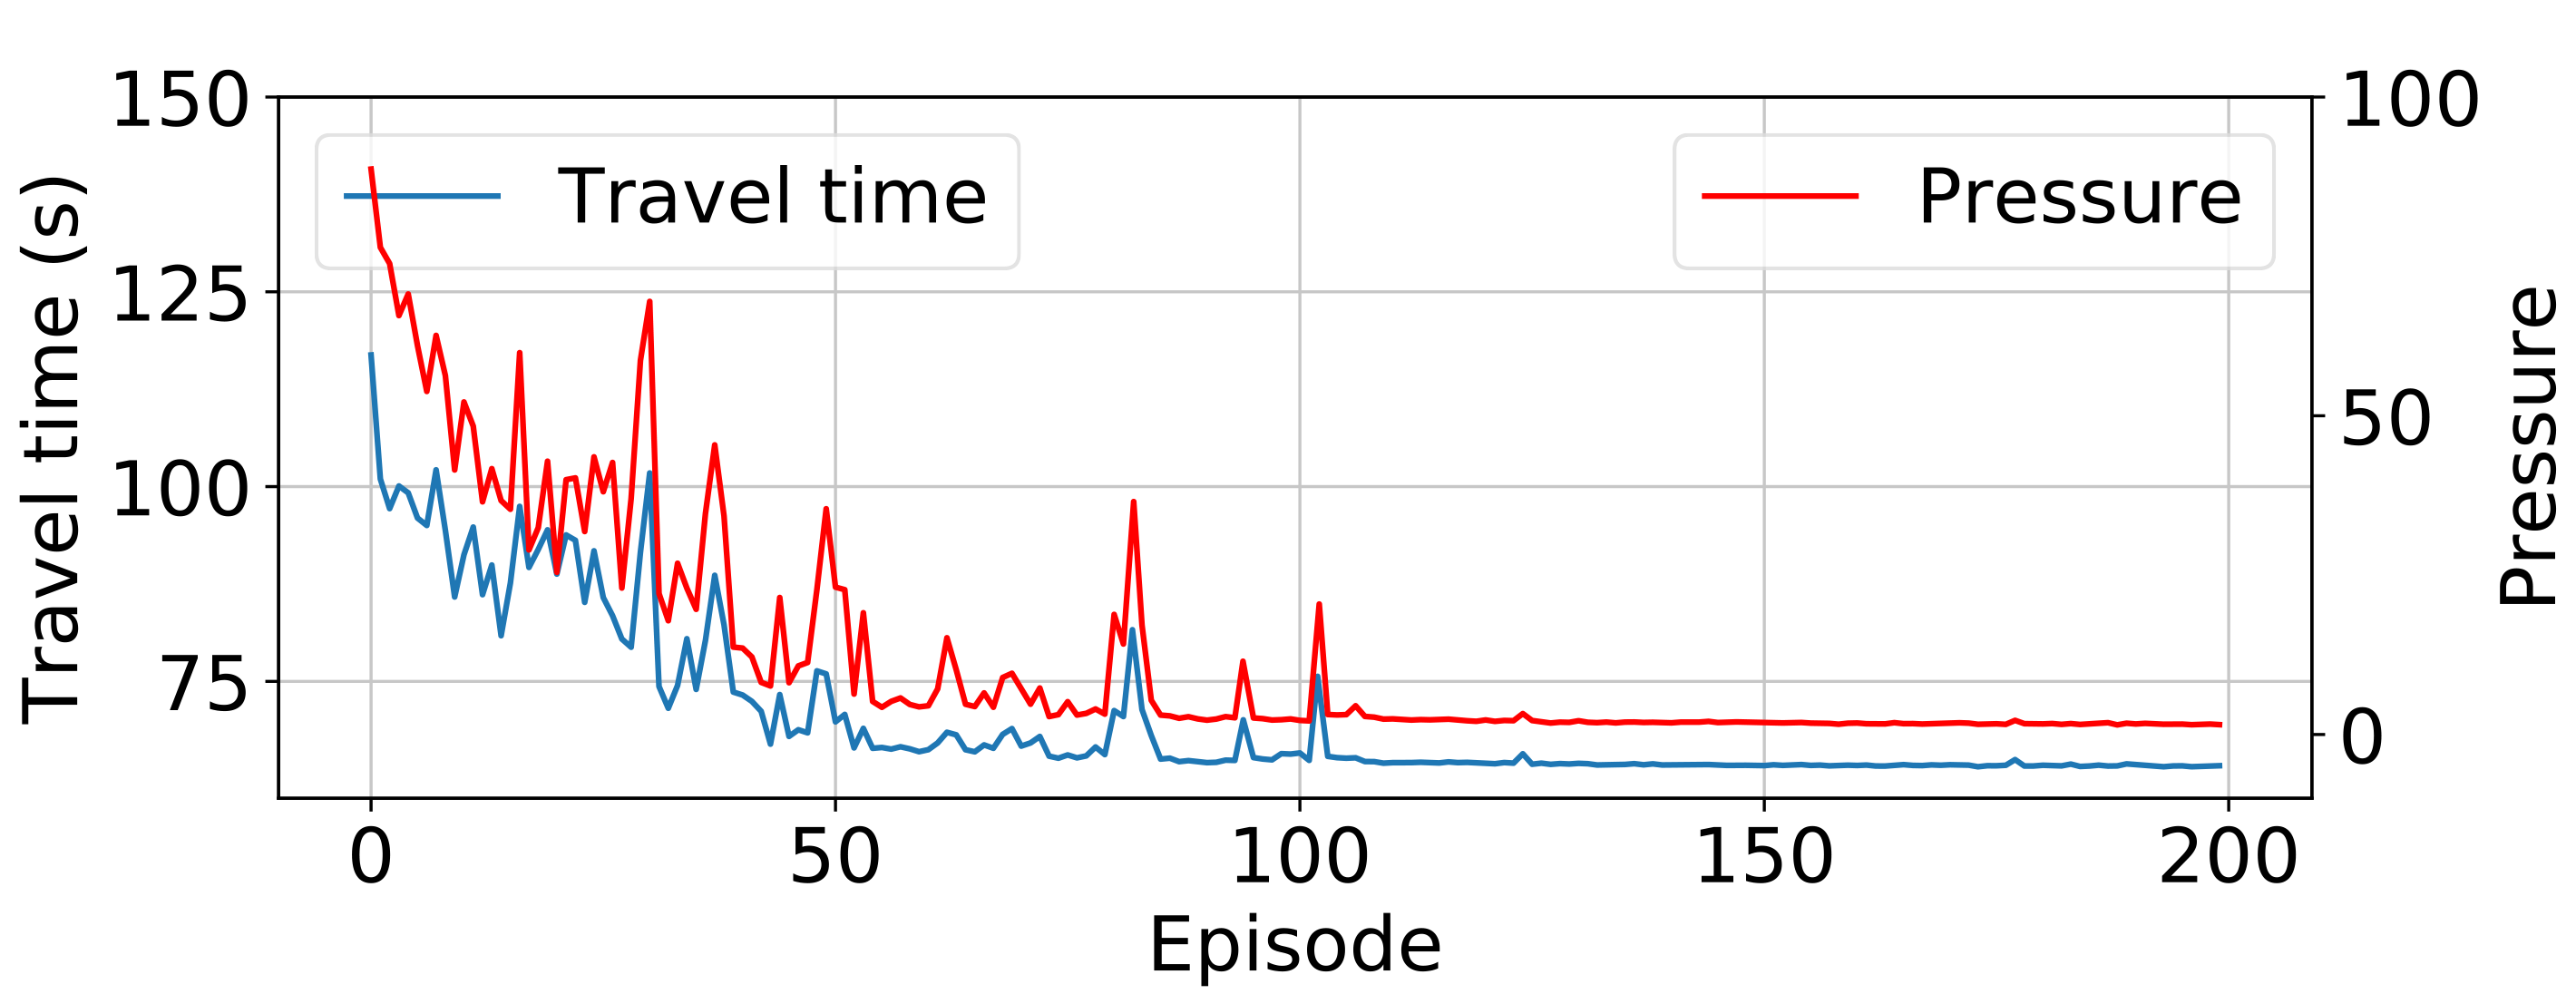
\includegraphics[width=1.0\textwidth]{figures/converg.png} \\
   \end{tabular}
   \end{center}
     \caption{Convergence curve of average duration and our reward design (pressure). Pressure shows the same convergence trend with travel time.}
    \label{fig:convergence}
\end{figure}

\subsection{Performance on Mixed Scenarios}

\subsubsection{Heterogeneous intersections}
We employ our model to two heterogeneous arterials, as is shown in Figure~\ref{fig:heter_inter}. For intersections with 3 legs, we use zero-padding to complete the state. For intersections with different lengths of lanes, our method can handle this well since the state is independent of the lane length. Table~\ref{tab:more-intersection} illustrates the performance of our model against \Maxpressure. 
% The conclusion could be drawn that our model could achieve better performance even when the intersections are heterogeneous.


\begin{figure}[t!]
\centering
   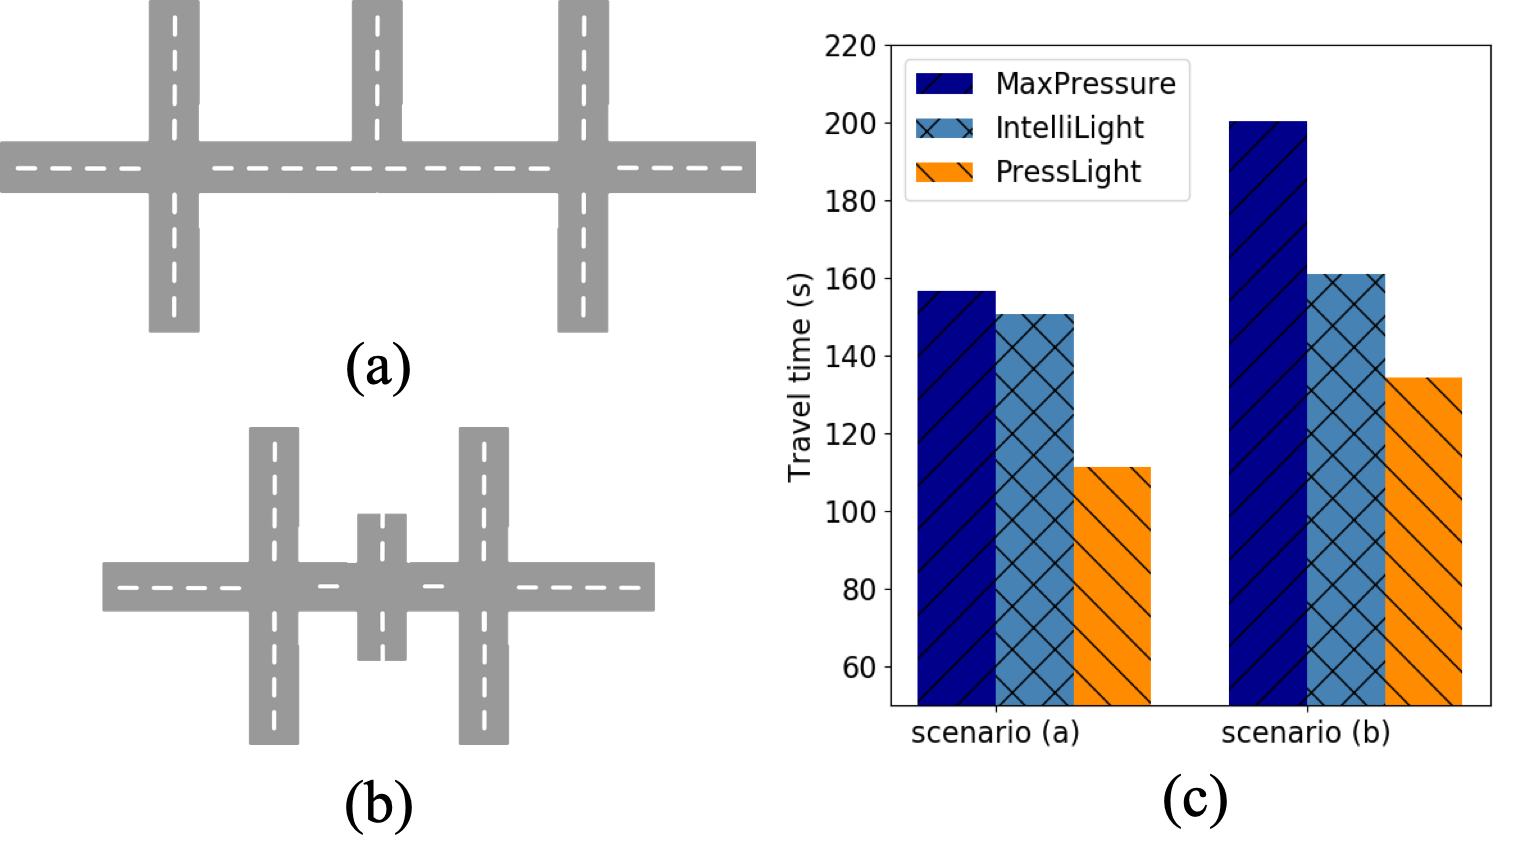
\includegraphics[width=0.8\textwidth]{figures/heter_results.png} 
     \caption{Average travel time of our method on heterogeneous intersections. (a) Different number of legs. (b)  Different length of lanes. (c) Experiment results.}
    \label{fig:heter_inter}
    % \vspace{-2mm}
\end{figure}
% \vspace{-2mm}

\begin{figure}[t!]
\centering
   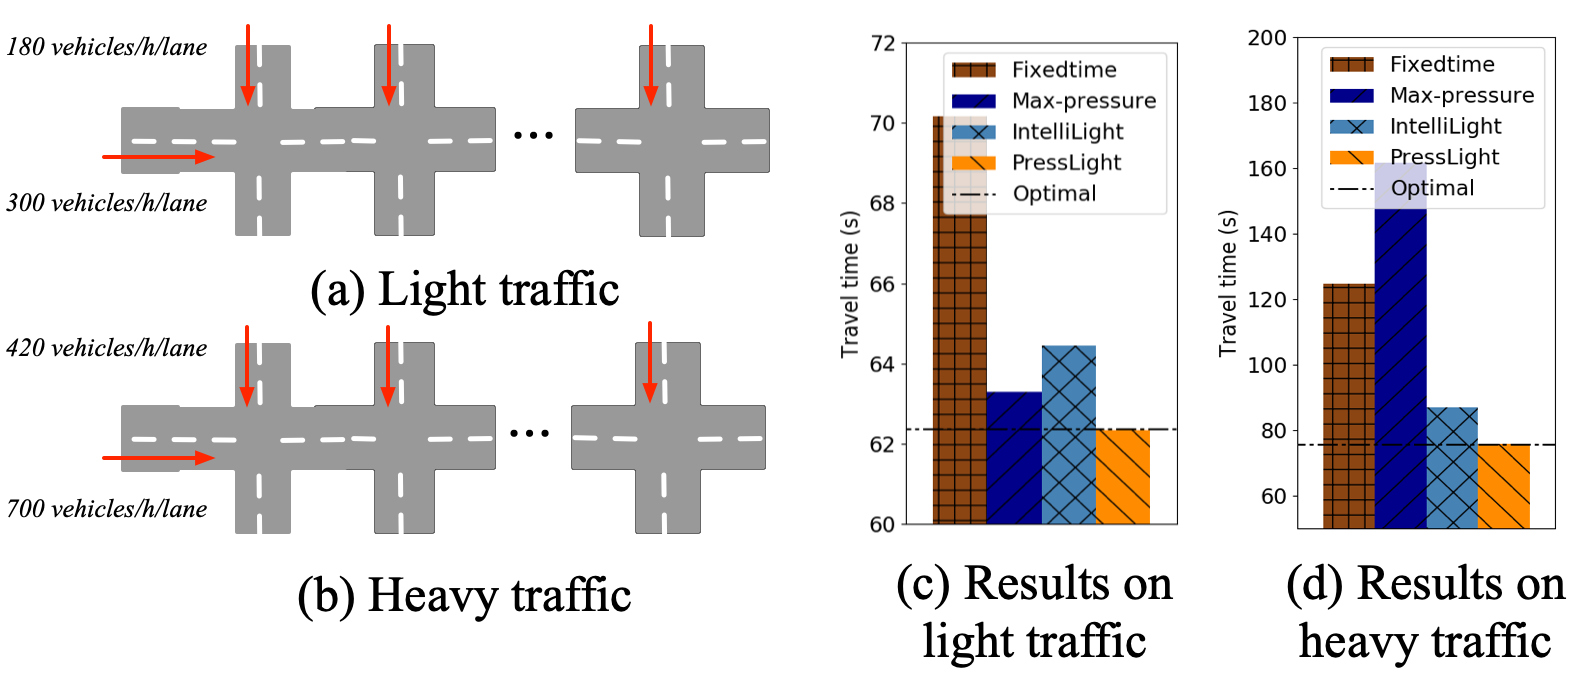
\includegraphics[width=0.9\textwidth]{figures/gw.png} 
     \caption{Performance comparison under uniform unidirectional traffic, where the optimal solution is known (\Greenwave). Only \PressLight can achieve the optimal.}
    \label{fig:optimal}
    % \vspace{-3mm}
\end{figure}

\subsubsection{Arterials with a different number of intersections and network}

\begin{table*}[t!]
\centering
\caption{Average travel time of different methods under arterials with a different number of intersections and network.}
\label{tab:more-intersection}
\begin{tabular*}{\textwidth}{ccccccc}
\toprule
           & \multicolumn{2}{c}{6-intersection arterial} & \multicolumn{2}{c}{10-intersection arterial} & \multicolumn{2}{c}{20-intersection arterial}  \\
           & \HeavyFlat  & \HeavyPeak & \HeavyFlat  & \HeavyPeak  & \HeavyFlat   & \HeavyPeak   \\ \midrule
\Maxpressure        &       262.26        &  225.60  &     129.63         &    129.63     &310.95 &    271.39                \\
\LIT        & 233.17  & 258.33     & 157.84 & 200.96 & 246.88 &  202.30     \\
\PressLight(ours) &  \textbf{160.48}  &  \textbf{184.51}   & \textbf{88.88}   &   \textbf{79.61}  & \textbf{155.84} & \textbf{188.92}           \\  \bottomrule
\end{tabular*}\\
\vfill
\vspace{1cm}
\begin{tabular}{ccc}
\toprule
           &  \multicolumn{2}{c}{Grid network} \\
           &  \HeavyFlat  & \HeavyPeak \\ \midrule
\Maxpressure              &   539.67           &     485.03        \\
\LIT         & 283.21  &    332.53      \\
\PressLight(ours)   \textbf{251.02} &  \textbf{262.46}           \\  \bottomrule
\end{tabular}
\end{table*}


% \begin{table}[tp!]
% \caption{(RQ3) Average travel time of different methods under synthesized traffic with different volumes. }
% \label{tab:RQ3-volume_comparison}
% \begin{tabular}{c|cccc}
% \toprule
%               & \multicolumn{4}{c}{Synthetic traffic }  \\ 
%               & \LightFlat & \LightPeak  & \HeavyFlat& \HeavyPeak  \\ \midrule
% \FT             &  93.29   		&   109.50        &    325.48       &   246.25         \\ 
% \Greenwave      &  98.39    	&  124.09         &   263.36        &   286.85         \\ 
% \Maxpressure    &  74.30       	&  82.37          &   262.26        &   225.60         \\ \hline
% \NIPS           &             	&                 &  525.64         &  757.73          \\
% \LIT      &  65.07       	&  66.77      	  &   233.17        &   258.33         \\ \hline
% \PressLight     &\textbf{59.96}	&  \textbf{61.34} & \textbf{160.48} &  \textbf{184.51} \\ 
% % Improvements &   7.85\%          &  8.13\%           &       5.69\%         &      31
% \bottomrule
% \end{tabular}
% \end{table}

We employ our model to arterials with 6, 10 and 20 intersections under synthetic data. As is shown in Table~\ref{tab:more-intersection},  our model could achieve better performance over conventional transportation method \Maxpressure and reinforcement learning method \LIT even when the number of intersections grows. 

We also test our model a network with 9 intersections ($3\times3$ grid). Table~\ref{tab:more-intersection} shows the experiment results and we can see that \PressLight can outperform \Maxpressure and \LIT under both traffic.

\subsection{Case Study}
Another desirable property of \PressLight is its ability to automatically coordinate the offset between adjacent intersections. To demonstrate this, we show two examples. Under simplified uniform traffic, we show that our model has learned the optimal solution which could be justified by transportation theories. Under the real-world traffic, the learned offset is visualized to reveal this property.
% and to optimize the offset between every two neighboring intersections which is because our designed state could capture the distribution of coming vehicles. To demonstrate this, we show two examples on uniform and real-world traffic.

\subsubsection{Synthetic traffic on the uniform, uni-directional flow}

In this section, we perform experiments on the arterials with six homogeneous intersections under two traffic settings. One is for light traffic (arterial demand: 300 vehicle/hour/lane, side-street demand: 180 vehicle/hour/lane) and one is for heavy traffic (arterial demand: 700 vehicle/hour/lane, side-street demand: 420 vehicle/hour/lane). Both of them are uniform and uni-directional without turning traffic and two phases (\WE for green light on arterial and \SN for green light for side streets) are used for all intersections. Under these simplified scenarios, the optimal solution is known as \Greenwave in transportation area as stated in ~\cite{Roess2011t}. As the optimal solution under these settings, \Greenwave's policy includes the offsets between intersections and the phase split, which requires several prior knowledge to calculate them: The offset $\Delta$ equals to the block length $l$ between two consecutive intersections divided by free-flow speed $v$; the optimal phase split ratio is equal to the ratio of the demand for a designated phase and total demand. In our experiments, $l\approx 300$ m, $v\approx 10$ m/s, hence, the optimal offset should be $\Delta\approx 30$ s, and the optimal phase split should be 1:0.6 (\WE : \SN).

\begin{figure}[t!]
  \centering
	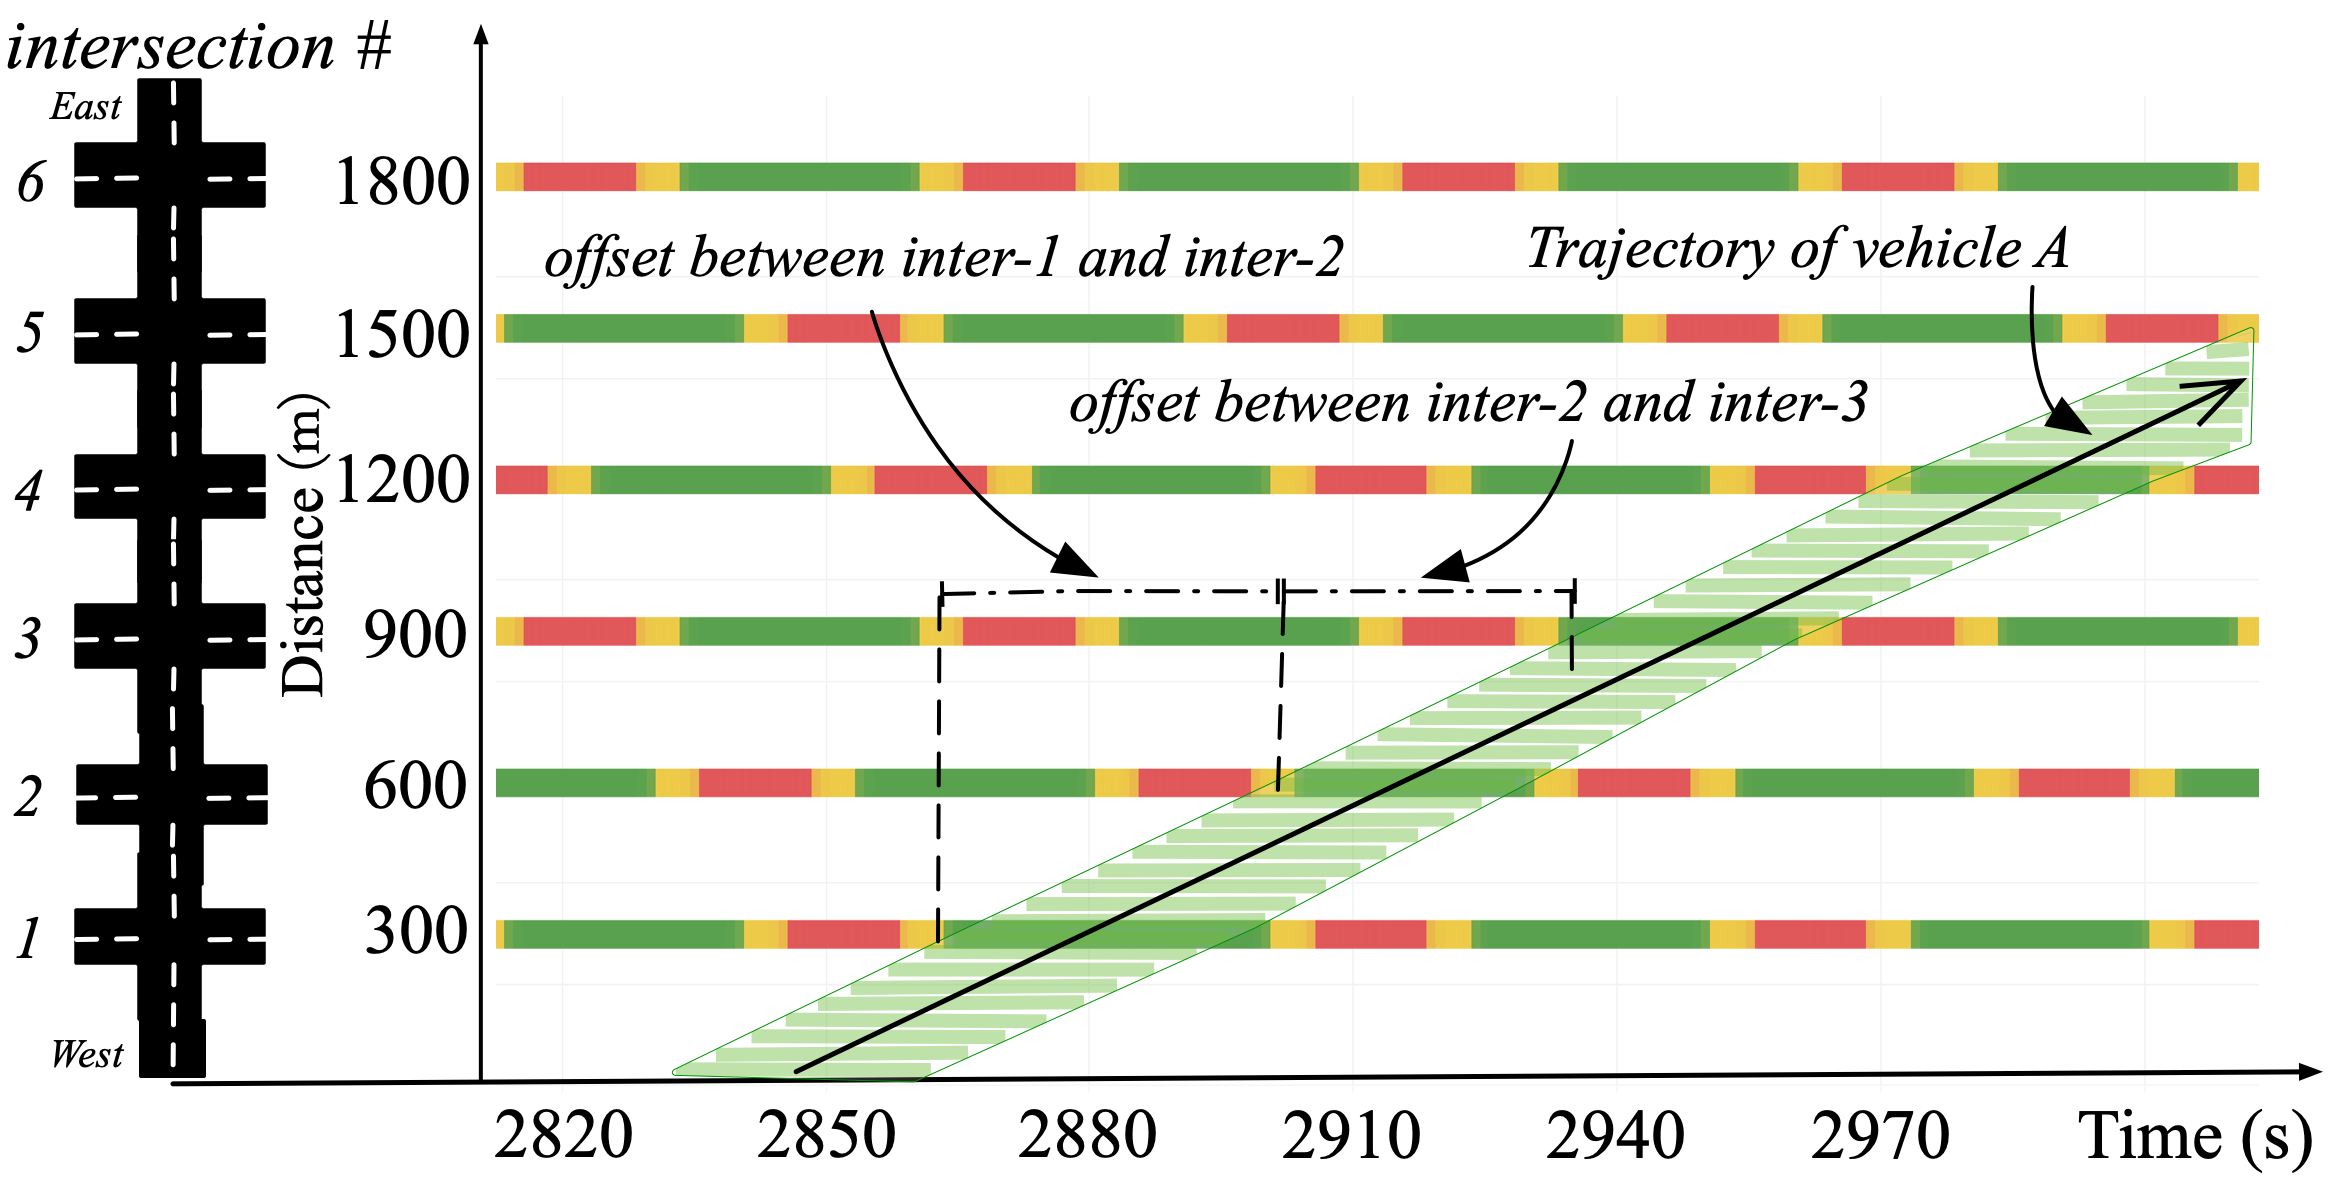
\includegraphics[width=0.8\textwidth]{figures/offset.png}
     \caption{Offsets between intersections learnt by RL agents under uni-directional uniform traffic (700 vehicles/hour/lane on arterial) }   
    \label{fig:case-study}
    % \vspace{-3mm}
\end{figure}

\begin{figure}[t!]
  \centering
  \begin{tabular}{c}
   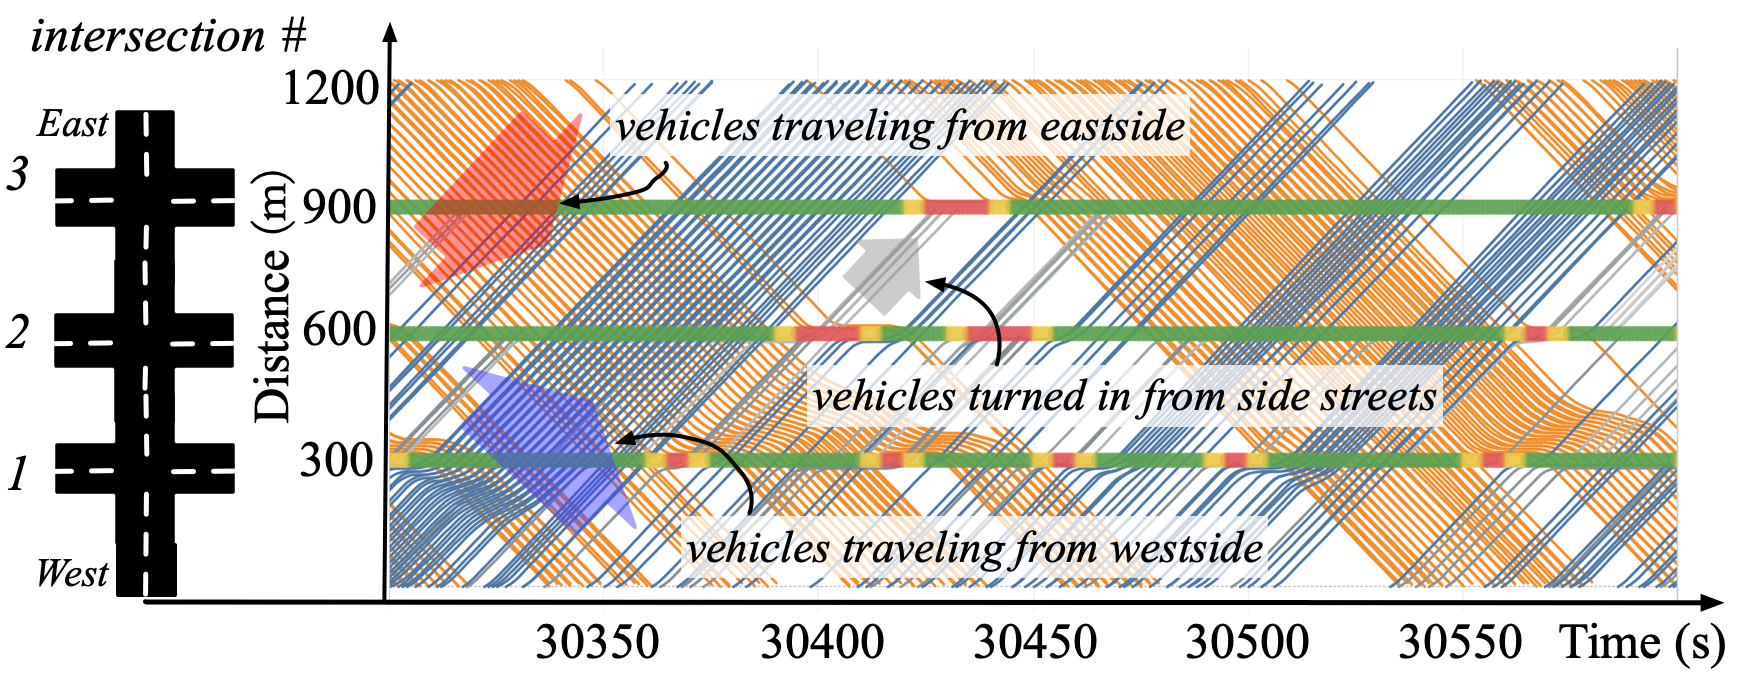
\includegraphics[width=0.8\textwidth]{figures/case_study_1.png} \\
   \end{tabular}
     \caption{Space-time diagram with signal timing plan to illustrate the learned coordination strategy from real-world data on the arterial of Qingdao Road in the morning (around 8:30 a.m.) on August 6th.}
    \label{fig:case-study-real}
    % \vspace{-3mm}
\end{figure}

\paragraph{Performance comparison}
We compared \PressLight with all aforementioned baselines and report their results in Figure~\ref{fig:optimal}. We can find that given \Greenwave is the optimal solution, only our method \PressLight achieves the same performance as \Greenwave in both settings. This demonstrates that our RL agents can learn the optimal policy under these simplified scenarios.


% \begin{figure}[t!]
%   \begin{tabular}{cc}
%   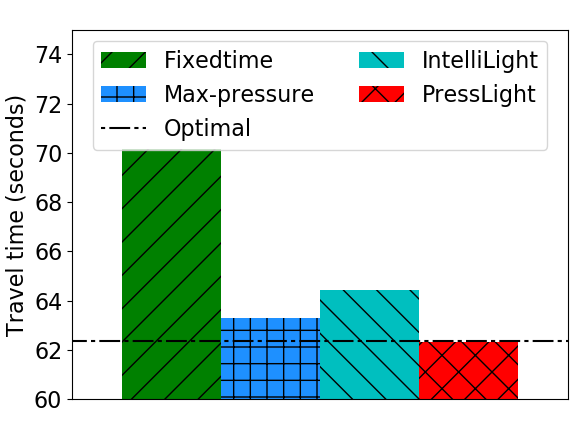
\includegraphics[width=0.22\textwidth]{figures/gw1.png} &
%   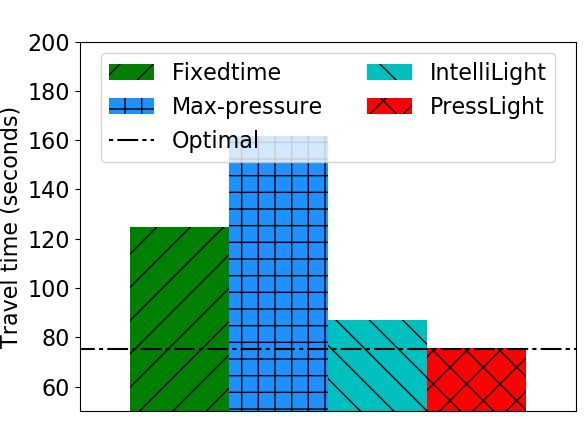
\includegraphics[width=0.225\textwidth]{figures/gw2.png} \\
%   \begin{tabular}[c]{@{}c@{}}(a) Light traffic\end{tabular}&
%   \begin{tabular}[c]{@{}c@{}}(b) Heavy traffic\end{tabular}\\
%   \end{tabular}
%      \caption{Performance comparison between all the methods under uniform unidirectional traffic. Under these situations, the optimal solution is known (\Greenwave). Only our method can achieve the optimal solution.}
%     \label{fig:optimal}
% \end{figure}

\paragraph{Policy learned by RL agents}
We use time-space diagrams to show the trajectories of vehicles and phase plans of traffic signal controllers. In a time-space diagram like Figure~\ref{fig:case-study}, the x-axis is the time and the y-axis is the distance (from a reference point, here we use the westernmost point as the reference point). As it is shown in Figure~\ref{fig:case-study}, there are six bands with green-yellow-red colors indicating the changing phases of six intersections. The black line with an arrow is the trajectory of a vehicle, where the x-axis tells the time and the y-axis tells the location. Vehicles that travel within the green dashed area will experience a green wave. For example, vehicle $A$ enters the system at 2850 second and traveled through 5 intersections at 3000 second, experiencing consecutive green lights during its trip. The slope indicates the speed of the vehicle. 

We have several observations:
\begin{enumerate}[wide,noitemsep,topsep=0pt]
    \item Our RL agents can learn the optimal phase split as \Greenwave.  As is shown in Figure~\ref{fig:case-study}, our method learns optimal phase split (approximately 1:0.6, with 25 seconds of \WE, 15 seconds of \SN, and 10 seconds of yellow light). 
    \item Our RL agents can learn the optimal offset and form a green wave. In Figure~\ref{fig:case-study}, the offset is approximately 30s between two consecutive traffic signals and a green wave can be seen (dashed green area in Figure~\ref{fig:case-study}). This demonstrates that our RL method can learn the optimal policy given by \Greenwave. 
\end{enumerate}

\subsubsection{Real-world traffic in Jinan}

In this section, we make observations on the policies we learned from the real data for the arterial of Qingdao Road ($East$ and $West$ direction) during the morning peak hour (around 8:30 a.m.) on August 6th.  In Figure~\ref{fig:case-study-real}, a time-space diagram is drawn with time on the horizontal axis and distance (from a reference point, here we use the westernmost point on the arterial as the reference point) on the vertical axis. Most of the blue and orange lines are straight, indicating most vehicles on the arterial are not stopped by red lights, which means our method can automatically form a green wave.

\section{Conclusion}
In this chapter, we propose a novel RL method for multi-intersection traffic signal control on the arterials. We conduct extensive experiments using both synthetic and real data and demonstrate the superior performance of our method over the state-of-the-art. Specifically, we draw a connection on the design between reinforcement learning with conventional transportation control methods. It is also the first time the individual RL model automatically achieves coordination along arterial without any prior knowledge. 
 
 We acknowledge the limitations of our model and would like to point out several future directions. In our experiment, we did not model the behavior of vehicles. The behavior of vehicles (e.g., routing) in the real-world may change dynamically in response to traffic lights. Another direction can be reducing the cost of learning. Since RL is learning from trial-and-error, deploying an online updated RL model in real-world could be dangerous and costly.


% \begin{acks}
% The work was supported in part by NSF awards \#1652525, \#1618448, and \#1639150. The views and conclusions contained in this chapter are
% those of the authors and should not be interpreted as representing
% any funding agencies.
% \end{acks}

% %%
% %% The next two lines define the bibliography style to be used, and
% %% the bibliography file.
% \bibliographystyle{ACM-Reference-Format}
% \bibliography{sample-base}

% %%
% %% If your work has an appendix, this is the place to put it.


% \end{document}
% \endinput
%%
%% End of file `sample-sigconf.tex'.

\chapter{Toward A Thousand Lights: Decentralized Deep ReinforcementLearning for Large-Scale Traffic Signal Control}
\label{chap:thousand}

\section{Preliminaries}
 
\begin{definition}[Traffic movement]
A traffic movement is defined as the traffic traveling across an intersection from one entering lane to an exiting lane. We denote a traffic movement from road $l$ to road $m$ as $(l,m)$. 
% We call $m$ is the downstream lane of $l$ and denote all the downstream lanes of $l$ as $Out_l$.
\end{definition}

\begin{definition}[Pressure of traffic movement]
Denote by $x(l,m)$ the number of vehicles for traffic movement $(l,m)$, the pressure of a traffic movement, $p(l,m)$ is simplely the difference between $x(l,m)$ and the average number of vehicles for all $l$'s downstream lanes.
    \end{definition}

% \chacha{Figure of MFD Fixedtime control}

\begin{problem}[Multi-intersection traffic signal control]
Each intersection is controlled by an RL agent. At time step $t$, agent $i$ views part of the environment as its observation $o^t_i$. Given the traffic situation and current traffic signal phase, the goal of the agent is to take an optimal action $a$ (i.e., which phase to set), so that the cumulative reward $r$ can be maximized. 
\end{problem}

% !TEX root = main.tex
\begin{figure}[t!]
\centering
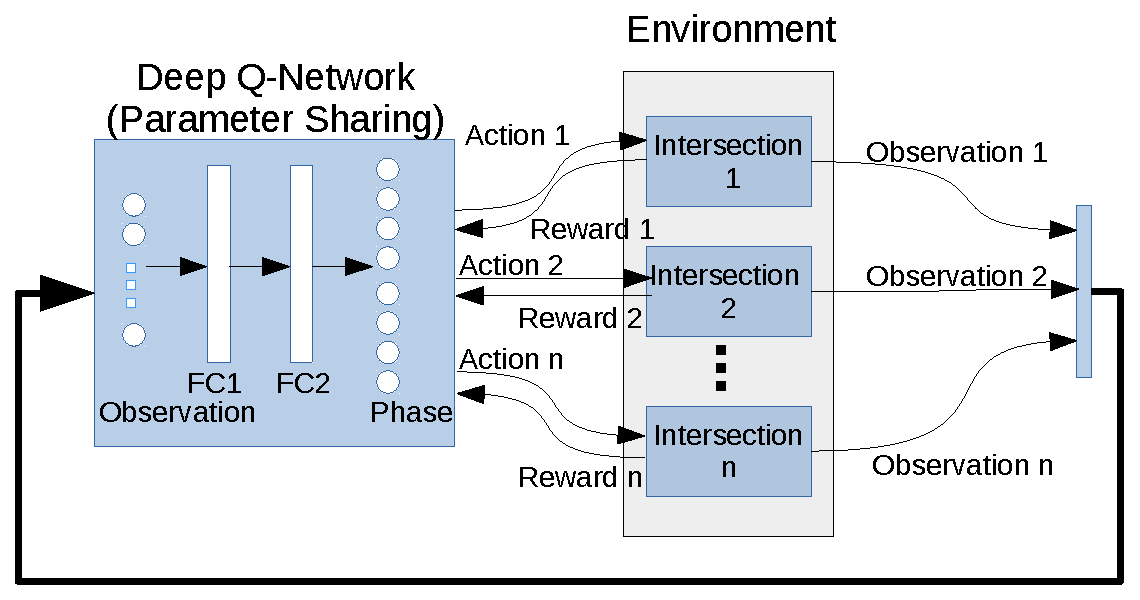
\includegraphics[width=.46\textwidth]{figures/framework.pdf}
%\vspace{-2mm}
\caption{The framework of \PressLight for multi-intersection signal control.}%\vspace{-2mm}
\label{fig:framework}
\end{figure}


\section{Method}
% We propose the decentralized reinforcement learning approach \PressLight for multi-intersection signal control. 

In this section, we first introduce the basic elements for reinforcement learning and describe the motivation of our novel reward design. Then we present the proposed \PressLight as a typical Deep Q-Network agent and show its learning process, as Figure~\ref{fig:framework} illustrates. For large-scale network signal control, we leverage parameter sharing among the agents, as discussed in the last part.

\begin{figure}[t!]
\centering
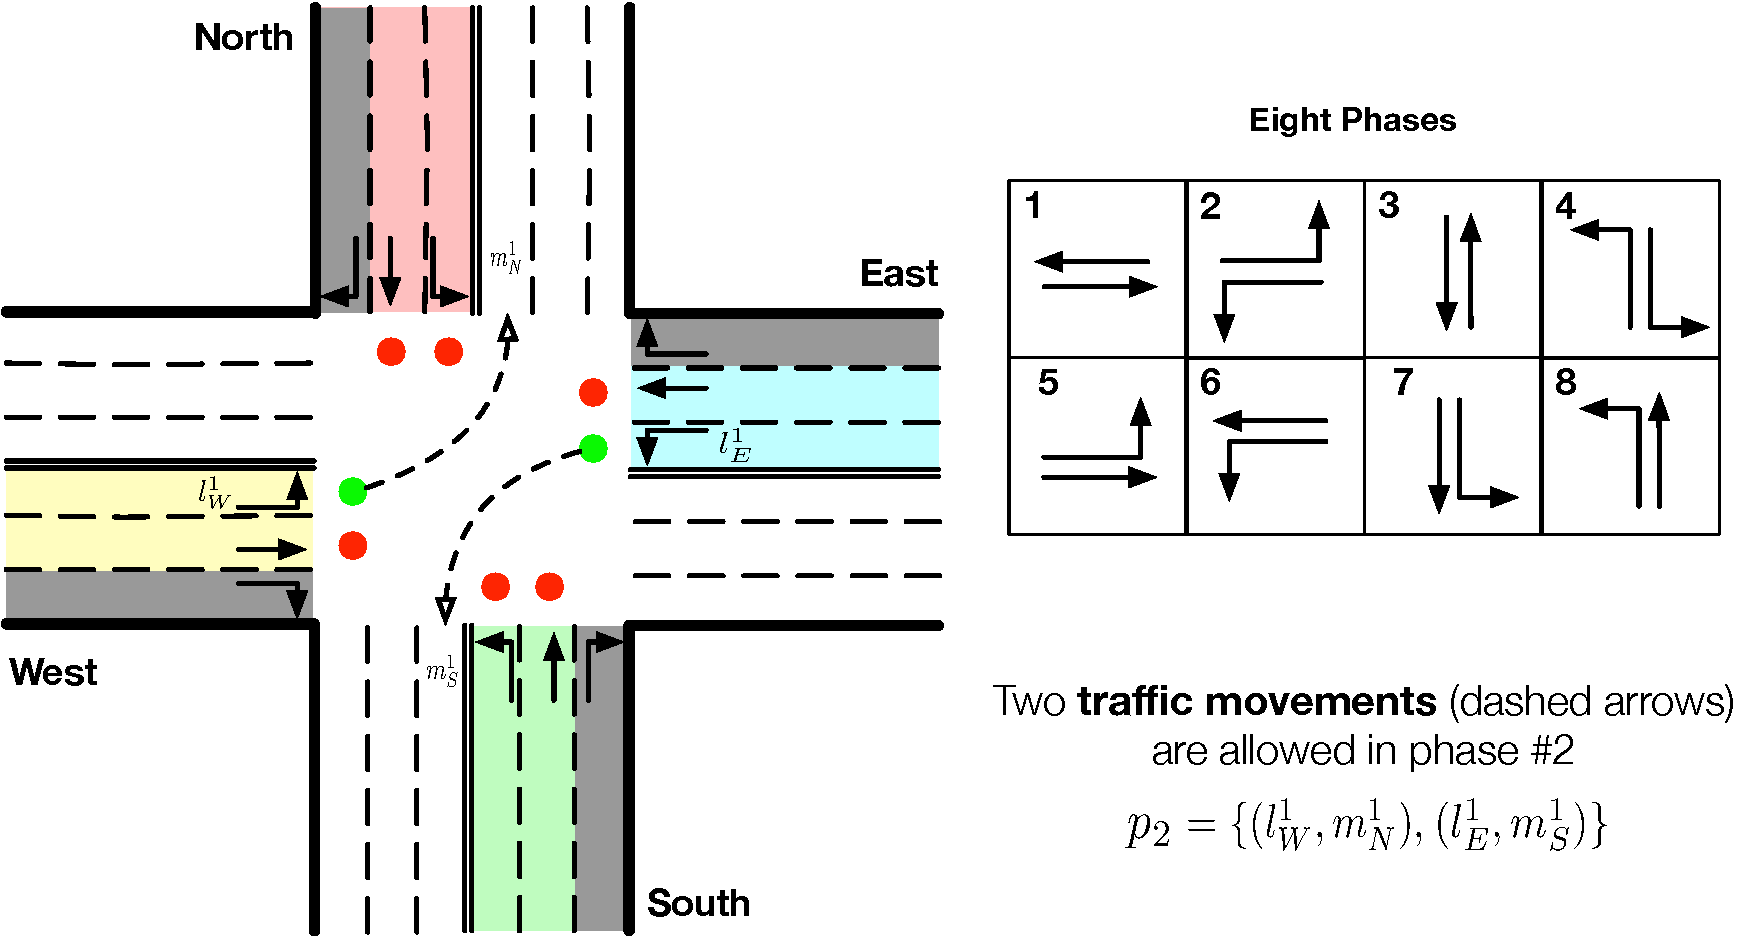
\includegraphics[width=0.36\textwidth]{figures/phase_detail.pdf} 
%\vspace{-2mm}
\caption{The illustration of an intersection with eight phases. In this case, phase \textbf{\#2} is set.}
%\vspace{-2mm}
\label{fig:phase}
\end{figure}

% Each intersection is controlled by an RL agent. An agent can only observe the local traffic situation (i.e. the traffic situation on all its entering and exiting approaches) and control the traffic signal accordingly. The goal of the agent is to learn a policy which maximizes its own long term cumulative reward.

% \subsection{Generic Model}
\subsection{Agent Design}
We design the state, the action as well as the reward for the \PressLight agent as follows.

\begin{itemize}
    \item \textbf{Observation}. Each agent observes part of the system state as its own observation. For a standard intersection with 12 traffic movements, its observation includes the current phase $p$ and the pressure of the 12 traffic movements. Note that for the intersection with fewer than 12 movements, the vector is zero-padded\footnote{In this paper, we only consider no more than 12 traffic movements, but the proposed method can be easily extend to control intersections with more than 12 movements.}.
    \item \textbf{Action}. 
         At time $t$, each agent chooses a phase $p$ as its action $a_t$, indicating the traffic signal should be set to phase $p$. 
         As shown in Figure~\ref{fig:phase}, eight phases are used to control the traffic movements in each intersection. For example, when phase \#2 is activated, the vehicles on the left-turn lane on the East and the West are allowed to turn left to their corresponding exiting lanes.
         
        %  Define agent (intersection) $i$'s action set as\\
        %  $A_i = \{(l,m) \text{for all the permissible traffic movement}\}$, 
         
        %  \WEs (going Straight from West and East), \SNs (going straight from South and North), \WEl (turning left from West and East), \SNl (turning left from South and North), \WW (going straight and turning left from West), \NN(going straight and turning left from North), \EE(going straight and turning left from East), \SSl(going straight and turning left from South).  


    %  At time $t$, each agent chooses a phase $p$ as its action $a_t$, indicating the traffic signal should be set to phase $p$. In our environment, Each action candidate $a_{i}$ is an one-hot vector representing a phase. 

    % Note that without loss of generality, in the grid road net setting, the set of actions only includes 4 phases while in the real-world scenario, it includes all the 8 phases. 


    \item \textbf{Reward}. In Figure~\ref{fig:pressure}, we define the reward $r_i$ for agent $i$ as the pressure on the intersection, which is simply the difference between the sum of the queueing vehicles on all the entering lanes and the sum of the queueing vehicles on all the exiting lanes.
    
    If we denote the pressure of intersection $i$ by $P_i$ , then the reward $r_i$ should be
        \begin{equation}
            \label{eq:reward-detail}
            r_i  = - P_i.
        \end{equation}
    By maximizing the reward, the agent is trying to stabilizing the queues in the system.
    \begin{figure}[htbp]
        \centering
        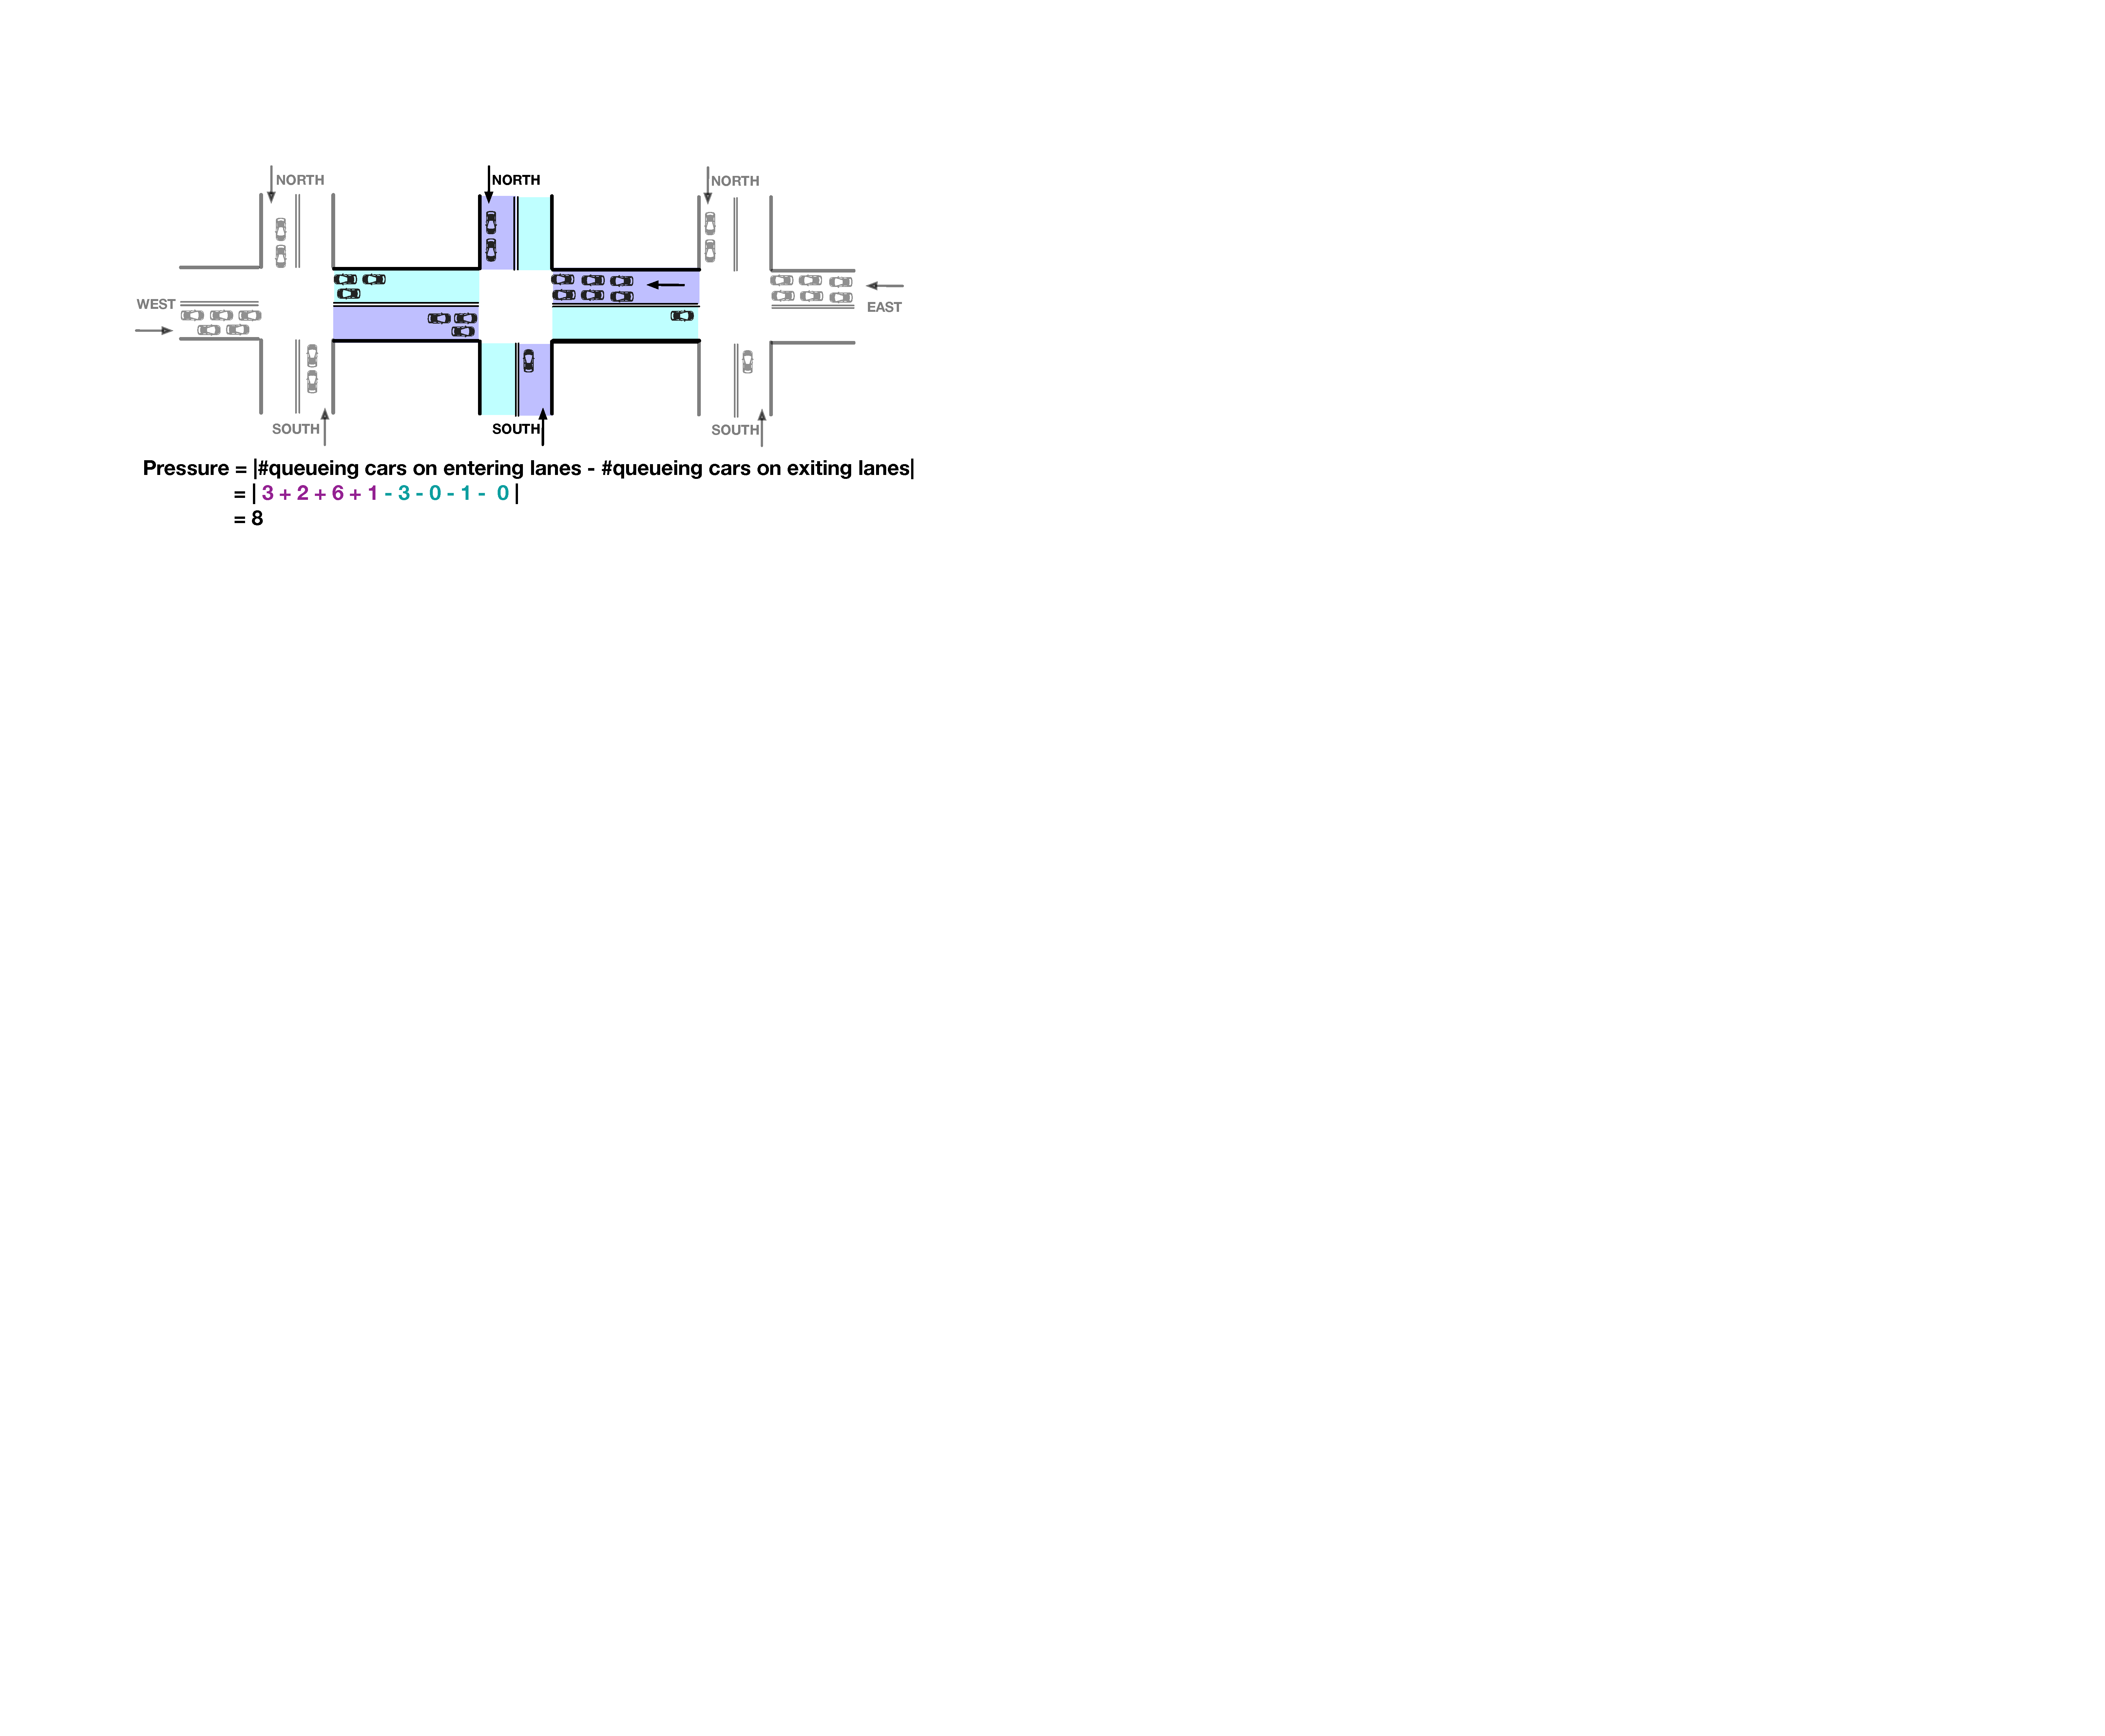
\includegraphics[width=0.5\textwidth]{figures/pressure_def.pdf} %\vspace{-2mm}
        \caption{The illustration of intersection pressure.}%\vspace{-2mm}
        \label{fig:pressure}
        \end{figure}
    % Intuitively, the By minimizing, the vehicles within the system can be evenly distributed. Then the green light is effectively utilized so that the throughput is optimized.
    % If we regard all the intersections have the same maximum capacity $x_{max}$ and $x(l,m)^{down}=\sum_{p\in Out_m}{r(m,p)\cdot x(m,p)}$ as the downstream number of vehicles and $x(l,m)$ as the upstream number of vehicles, then 
    % \begin{equation}
    % w(l,m)= x(l,m)-x^{down}(l,m)
    % \end{equation}
    % is simply \textit{the difference between the upstream and downstream number of vehicles}. If the vehicles are not allowed to change their lanes, then $|Out_m|=1$ and $r(m,p)=1$, we have $w(l,m)= x(l,m)-x(m,p)$, which is simply the difference of number of vehicles between the upstream and downstream lane.
\end{itemize}


\subsection{Reward Function Verification}
In previous work~\cite{varaiya2013max}, max pressure control law utilized only local information at each intersection under infinite capacities and has been proved to be stability-optimal, i.e., stabilizing and maximizing the throughput. In practice, however, max pressure control is often implemented in a greedy manner, which leads to a local optimum, see Algorithm~\ref{alg:mp}.
% Basically, max pressure control greedily searches the phase to set which minimize the pressure of an intersection.
% Our reward design match the objective of max pressure control law. Each individual agent maximizes its own reward.


\begin{algorithm}[H]
% \SetAlgoLined
% \KwResult{Write here the result }
%  initialization\;
\For{each intersection $i$}{
\For{each traffic movement (l,m)}
{   
calculate $p(l,m)$
}
next phase $\leftarrow \arg\max \{p(l,m) |\text{if $(l,m)$ is permissible} \} $ 

}


%  \While{While condition}{
%   instructions\;
%   \eIf{condition}{
%   instructions1\;
%   instructions2\;
%   }{
%   instructions3\;
%   }
%  }
 \caption{Max Pressure Control}
 \label{alg:mp}
\end{algorithm}


By setting the reward of our RL agents to be the same as max pressure control objective, each local agent is maximizing its own cumulative reward, which further maximizes the network throughput under certain constraints.



%  The key idea of MP is to minimize the ``pressure'' of an intersection., which can be loosely defined as number of vehicles on entering lane minus the number of vehicles on exiting lane. Figure~\ref{fig:pressure} illustrates the concept of pressure. By setting the objective as minimizing the pressure of intersections, MP is proved to maximize the throughput of the whole road network\footnote{Maximizing throughput equals to minimizing travel time under certain conditions and minimizing travel time is the final goal for traffic signal control.}. However, the solution of MP is greedy which leads to locally optimal solutions. 
 
%  \chacha{todo}
 


% MARL with parameter sharing network
% because all the agent should ultimately converge upon the same value function

\subsection{Deep Q-learning}
As shown in Figure~\ref{fig:framework}, we use a Deep Q-Network (DQN) to solve the multi-intersection signal control problem. Basically, our DQN network takes the state features on the traffic movements as input and predicts the score (i.e., Q value) for each action candidate (i.e., phase) as described in the following Bellman Equation:
\begin{equation}
Q(s_t,a_t)=R(s_t, a_t)+\gamma \max Q(s_{t+1}, a_{t+1}).
\label{eq:bellman}
\end{equation}

\PressLight predicts the action for intersection $i$ at time $t$ as follows.
\begin{eqnarray}
h^i_{1,t}&=&\text{FC1}(o^i_t),\\
h^i_{2,t}&=&\text{FC2}(h^i_{1,t}),\\
\widetilde{q}&=&h^i_{2,t}W_p+b_p,
\end{eqnarray}
where FC1 and FC2 are two consecutive fully connected layers with ReLU as the activation function, $W_p$ and $b_p$ are the trainable weight and bias in the last q-value prediction layer.

Hence the loss function for our \PressLight to optimize the current policy is:
\begin{equation}
L(\theta)=\frac{1}{T}\sum_{t=1}^{t=T}\sum_{i=1}^{i=N}\big(q(o^i_t,a^i_t)-\widetilde{q}(o^i_t;a^i_t,\theta)\big)^2,
\end{equation}
where $q(o^i_t,a^i_t)$ and $\widetilde{q}(o^i_t;a^i_t,\theta)$ are the targeted and predicted q values for intersection $i$ at time step $t$, respectively, $T$ is the total number of time steps for sampling, $N$ is the number of intersections in the road network, $\theta$ is the variable to learn by \PressLight.


\subsection{Parameter Sharing} 
In Figure~\ref{fig:framework}, parameters of the network are shared among all the agents. The single \PressLight model receives observations from different agents to predict the corresponding actions and learns from environment rewards for parameter update. Note that the replay memory is also shared so that all the agents can benefit from experiences of the others.

% \subsection{Agent Overview}





% To address this setting, we formulate two approaches. The first, reinforced inter-agent learning
% (RIAL), uses deep Q-learning [3] with a recurrent network to address partial observability. In one variant of this approach, which we refer to as independent Q-learning, the agents each learn their own network parameters, treating the other agents as part of the environment. Another variant trains a single network whose parameters are shared among all agents. Execution remains decentralised, at which point they receive different observations leading to different behaviour.

% \subsection{Problem Definition}
% (RL for Multi-intersection Traffic Signal Control) In an arterial with multiple intersections, the traffic signal lights in each of the intersection is controlled by an RL agent. 
% We aim to:
% \begin{itemize}
%     \item Find a RL algorithm that can maximize the road network throughput.
%     \item Connect the RL algorithm with classical transportation theory, and prove the optimality of our RL algorithm with the concise state and reward definition.
% \end{itemize}




% \subsection{State Reweard design}
% \begin{itemize}
%     \item State : concise state -- onemodel (large-scale)
%     \item Reward : theoretically provable in transportation
% \end{itemize}


% \subsection{Model framework: Individual RL agent}
% In this section, we present our RL model framework. The action, state and reward design are fully justified with the connection to traditional traffic control strategy. 
% \subsubsection{Notation}
% \begin{table}[H]
% \centering
%   \caption{Notation}
%   \label{tab:notation}
%   \begin{tabular}{ll}
%     \toprule
%     Notation&Meaning\\
%     \midrule
%     $s$      & State      \\
%     $a$        & Action      \\
%     $r$        & Reward       \\
%     $\mathcal{L}$ & \begin{tabular}[l]{@{}l@{}}set of internal links where the starting and end of \\ 
%     the link are inside the system \end{tabular} \\
%     $\mathcal{L}_{entry}$ & \begin{tabular}[l]{@{}l@{}}set of entry links, where only end of the link is \\ inside the system \end{tabular} \\
%     $In_l$ & Set of links input to l\\
%     $Out_l$ & Set of links output from l\\
% 	$(l,m)$ & a phase that a green signal is on from link $l$ to $m$\\
%     $x(l,m)$ & number of vehicles leaving $l$ and entering $m$\\
%     $x_{max}(l,m)$ &capacity of link $l$ \\
%     $r(l,m)$ & turning ratio of  $m$\\
%     $c(l,m)$ & discharge rate of phase $(l,m)$, vehicles per timestep\\
%     $C(l,m)$ & saturation flow of phase $(l,m)$, vehicles per timestep\\
%     $\mathcal{N}$ & set of nodes or intersections, elements $n$\\
%     % $q_i $ & Queue length on the lane $i$ \\
% % 	$v_i$ & Number of vehicles on the lane $i$ \\
% 	$S_{n}$ & a control matrix (stage) for the intersection $n$\\
% 	$\mathcal{S}_n$ & \begin{tabular}[l]{@{}l@{}}set of the acceptable control matrices for the \\
% 	intersection $n$ \end{tabular}\\
% 	$P_i$ & pressure on intersection $n$\\
%     $L$ & length of a road segment\\
% 	  \bottomrule
% \end{tabular}
% \end{table}

% \subsection{Action}
% \subsubsection{Phase Selection}
% The action of our agents is set to be a phase chosen from 4 predefined phases. 
% \begin{itemize}
% \item WSES
% \item NSSS
% \item WLEL
% \item NLSL
% \end{itemize}


% \subsection{State}


% We first define $X(n)$ to be the array of numbers of vehicles on links adjacent to node $n$.
% \begin{equation}
% X(n)=\{x(l,m)\ |\ (l,m)\in \mathcal{S}_n \}
% \end{equation}

% In order to capture the changing dynamic of each lane, we break down each lane to segments with length $L$. Denote by $<x(l,m)_1,...,x(l,m)_k>$ the array of the number of vehicles of each road segment. Suppose the segment nearest to the intersection is the first segment, e.g. $x(l,m)_1$. In the state design, we only care about the first 3 road segments.

% Define 
% \begin{equation}
% X(i)_1 = \{x(l,m)_1||x(l,m)_2||x(l,m)_3|(l,m)\in \mathcal{S}_n\}
% \end{equation}

% The state of an individual RL agent $i$ is defined as
% \begin{equation}
%    s_i = X(i_1)||X(i_2)||X(i_3)
% \end{equation}

% Note that there is an assumption of length $L$ that $3\times L$ is no longer than the shortest lanes for any intersections.

% The state of an individual RL agent $i$ is defined as
% \begin{equation}
%    s_i = X(i_1)||X(i_2)...||X(i_k) 
% \end{equation}
% $X(i_k)$
% \begin{equation}
% X(n)=\{x(l,m)|(l,m)\in \mathcal{S}_n \}
% \end{equation}
% the array of queues on links adjacent to node $n$. For intersections without upstream or downstream neighbors, the entries are all set zero.


% \subsubsection{Store and Forward Model}

% What's the relationship between SF model and RL environment.
% We recall the store-and-forward queuing network model of the movement of individual vehicles from one link to another, and define what it means for a feedback (e.g., RL) control to be stabilizing. 
% See Fig 2. associate a distinct queue with each link $l\in\mathcal{L}\cup\mathcal{L}_{entry}$ and each $m\in Out_l$, and let $x(l,m)(t)$ be the length of this queue at the beginning of period $t$. Let $X(t)={x(l,m)(t)}$ be the array of all the queue lengths. $X(t)$ is the \textit{state} of the queuing network. $\mathcal{X} = {{x(l,m)\geq 0}}$ is the the state space.
% At the end of each period $t$ a control matrix $a(t)={a(l,m)(t)}\in \mathcal{A}$ must be selected as a function of $X(t)$ for use in period $(t+1)$, see Fig.2. Thus $a(t)=u(X(t))$ is given by a RL control policy $\pi:\mathcal{X}\rightarrow\mathcal{A}$.

% \subsubsection{Markov chain queuing process} 
% For each $l,m$ and $t$, the service rate $c(l,m)(t+1)$, turn ratio $r(l,m)(t)$ and demands $d(l,m)(t+1)$ are independent of $X(1),...,X(t)$, the process $X(t),t=1,2,...$ is a Markov chain. The transition probabilities and hence the statistics of the chain $X(t)$, depend on the RL control policy $\pi$.
% We now develop the equations of evolution of the state $X(t)$. First consider an internal link $l\in\mathcal{L}$. Suppose $a(l,m)(t) = 1$, that is phase $(l,m)$ is actuated. Then up to $c(l,m)(t+1)$ vehicles will leave queue $(l,m)$ and they will be routed to queue $(m.p)$ with probability $r(m,p)(t)$. So at the beginning of period $(t+1)$, $x(l,m)$ will decrease by up to $c(m,p)(t)$ and $x(m,p)$ will increase by the same number. This processes are captured by queue evolution equation: 
% \begin{align*}
% x(l,m)(t+1) =x(l,m)(t)-\min[C(l,m)(t+1)S(l,m)(t),x(l,m)(t)]\\
% +\sum_k\min[C(k,l)(t+1)S(k,l)(t),x(k,l)(t)]R(l,m)(t+1)\\
%  l\in\mathcal{L}, m\in Out_l
% \end{align*}

% \subsubsection{System Stability}
% Following the definition in [ref2], we define the system stability as 
% \begin{definition}[Dynamic Features]\label{def:dynamic}
% \end{definition}
% \theoremstyle{Definition}
% \begin{definition}{System stability}
% The queue length process $X(t) = \{x(l, m)(t)\}$ is stable in the mean (and $u$ is a stabilizing control policy) if for
% some $K<1$
% \begin{equation}
%     \sum_{t=1}^{T}\sum_{(l,m)}Ex(l,m)(t)<K, \quad\text{for all $T$.}
% \end{equation}
% Stability in the mean implies that the chain is positive recurrent and has a unique steady-state probability distribution. In(1), $E$ denotes expectation.
% \end{definition}

% \subsection{Reward}
% We define the reward of our RL agent similar to the definition of pressure in Max-pressure, where we try to maximize the reward, a.k.a., minimize the pressure of the intersection:
% \begin{equation}
% \label{eq:reward}
%     r(n)(t) = - P(n)(t)
% \end{equation}
% where: 
% \begin{subequations}
% \label{eq:reward-detail}
% \begin{align}
% P(n)(t) & = \sum_{(l,m)\in n}w(l,m)(t)\\
% \intertext{$P(n)(t)$ denote the defined pressure on intersection $n$ at time $t$.}
% w(l,m) & = |\frac{x(l,m)}{x(l)}-\sum_{k\in Out_m}\frac{r(m,p)x(m,p)}{x(m)}|\\
% n & \in\mathcal{N}
% \end{align}
% \end{subequations}

% !TEX root = main.tex
\section{Experiments}
In this section, we conduct extensive experiments to answer the following questions:
\begin{itemize}
	\item \textbf{RQ1}: Can the proposed \PressLight outperform the state-of-the-art methods for signal control in different road networks?
\	\item \textbf{RQ2}: How is the road resources utilized by \PressLight?
% 	\chacha{I dont understand..}
% 	Why it is useful or valid for a region level control using individual agent?
	% In network level, what is our RL agent 
	% Interpretating our policy using MFD? In network level, why is one policy better than another? (case study 2)
	% \item \textbf{RQ3}: Why delta q as reward is better than q (to validate our reward design), especially in peak hour (case study 2) 
	\item \textbf{RQ3}: What impact does the parameter sharing leveraged in \PressLight have on model learning?
	\item \textbf{RQ4}: Is \PressLight scalable enough to control all the signals in a modern city?
\end{itemize}




\subsection{Settings}
Following the previous work on traffic signal control study~\cite{wei2018intellilight}, we conduct experiments on SUMO (Simulation of Urban MObility)\footnote{https://sourceforge.net/projects/sumo/}. In order to support large-scale reinforcement learning, we implement the multi-thread version of SUMO. After the traffic data being fed into the simulator, a vehicle moves towards its destination according to the setting of the environment. The simulator provides the state to the signal control method and executes the traffic signal actions from the control method. Following the tradition, each green signal is followed by a three-second yellow signal and two-second all red time\footnote{The codes and the public datasets used in this paper are available online: \url{https://www.dropbox.com/sh/tx81ndkiqdpk784/AACfJk7wUu-cFElm7uiuURRda?dl=0}}. 

In a traffic dataset, each vehicle is described as $(o, t, d)$, where $o$ is the origin location, $t$ is  time, and $d$ is the destination location. Locations $o$ and $d$ are both locations on the road network. Traffic data is taken as input for the simulator.

In a multi-intersection network setting, we use the real road network to define the network in the simulator. Unless specified, each intersection in the road network is set to be a four-way intersection, with four 300-meter long road segments. 

\subsubsection{Datasets}
Both synthetic and real-world datasets, which focus on bi-directional and dynamical flows with turning traffic, are used in our experiments. The two kinds of datasets are described as follows.
\begin{itemize}[wide,noitemsep,topsep=0pt]
\item Synthetic data on a $4\times4$ network shown in Figure~\ref{fig:net}. As listed in Table~\ref{tab:synthetic-table}, four configurations are used to test the signal control models in different traffic demands: two types of vehicles' average arriving rate, each with Flat (0.3 variance) and Peak (0.6 variance) patterns. 


% Synthetic data on a $4\times4$ network shown in Figure~\ref{fig:net2}, the data statistics is the same. This smaller road net is used to efficacy of the parameter sharing for convenience. Because without parameter sharing, the training process is quite computation resource consuming. 

\begin{figure}[htbp]
\centering
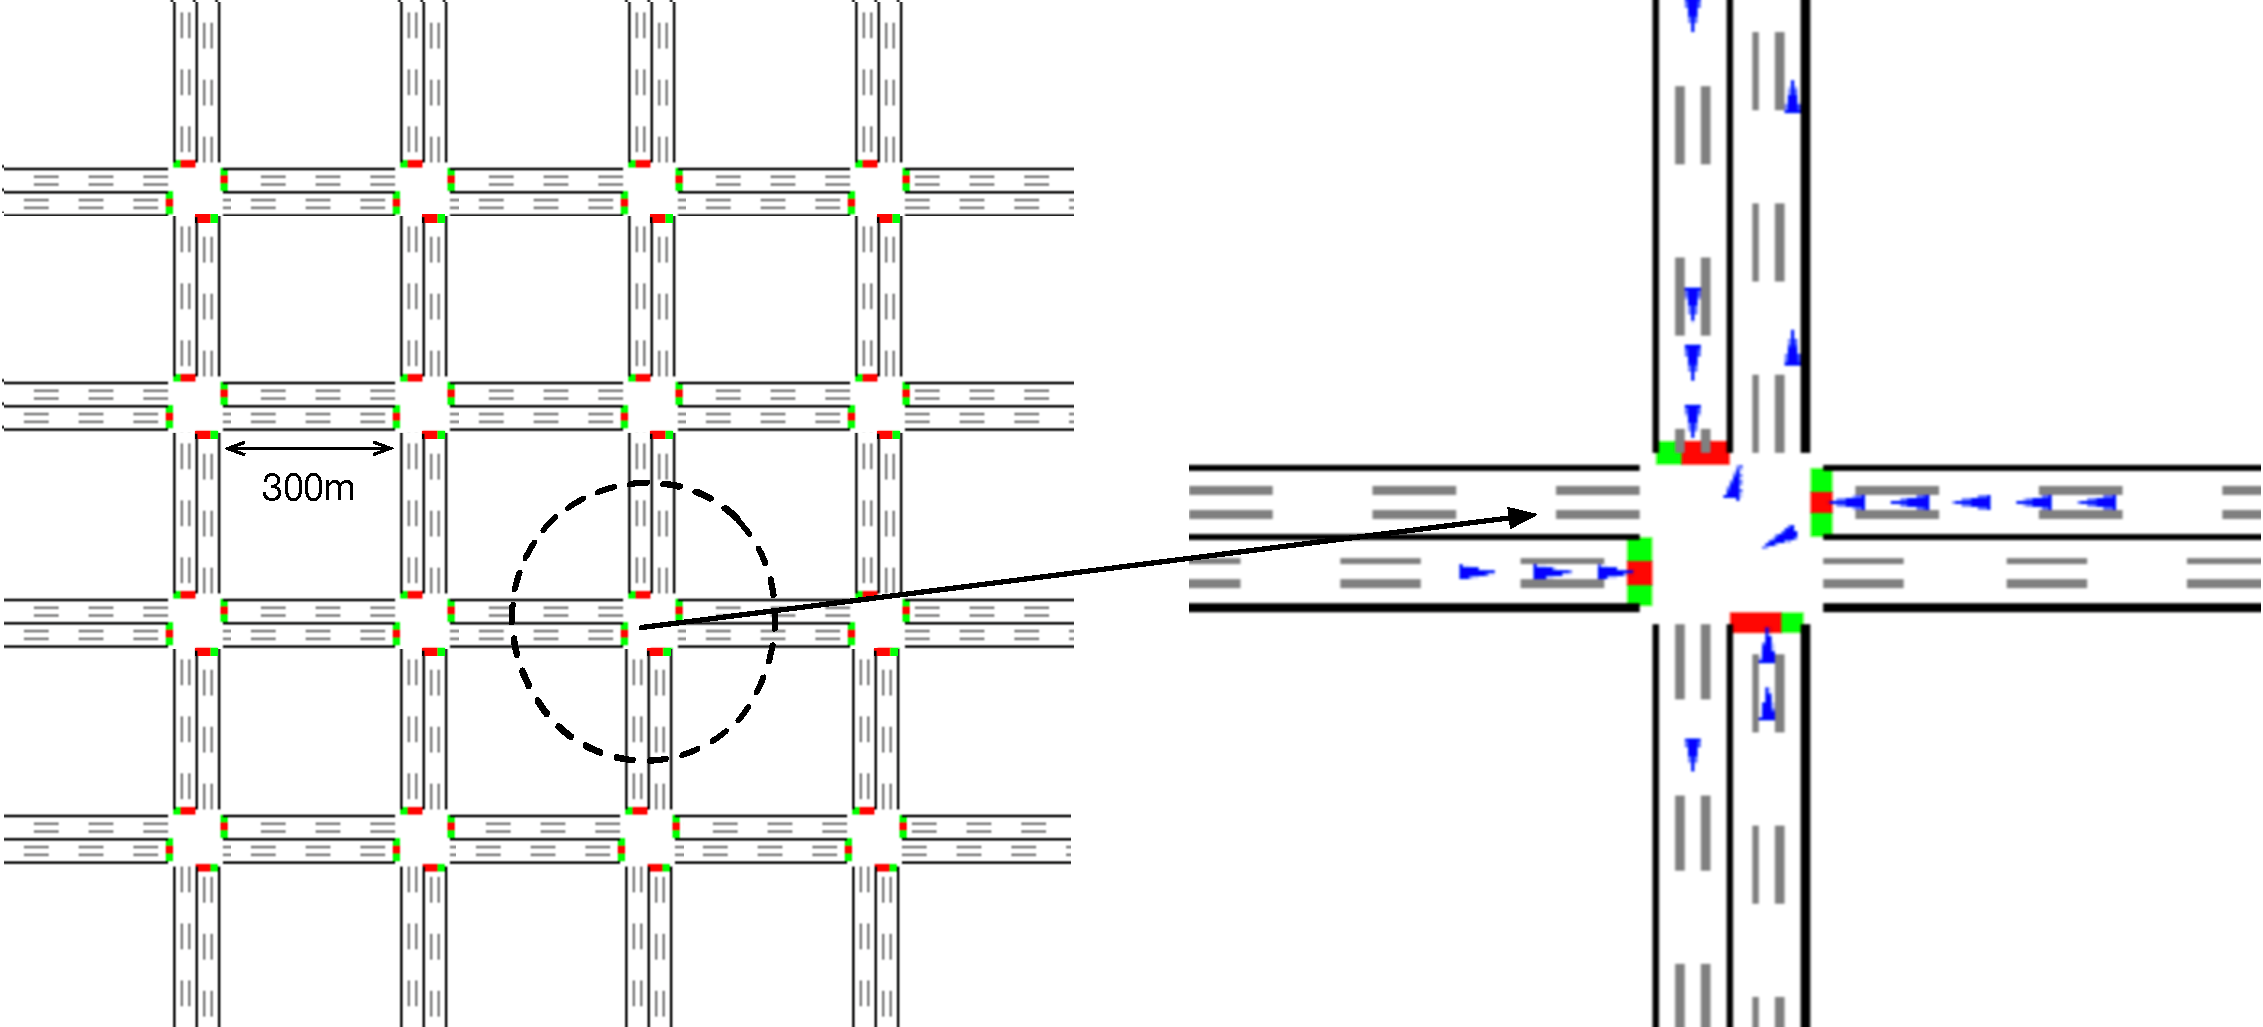
\includegraphics[width=0.5\textwidth]{figures/road_net.pdf} \vspace{-2mm}
\caption{$4\times4$ road network.}\vspace{-2mm}
\label{fig:net}
\end{figure}

% \begin{figure}[htbp]
% \centering
% 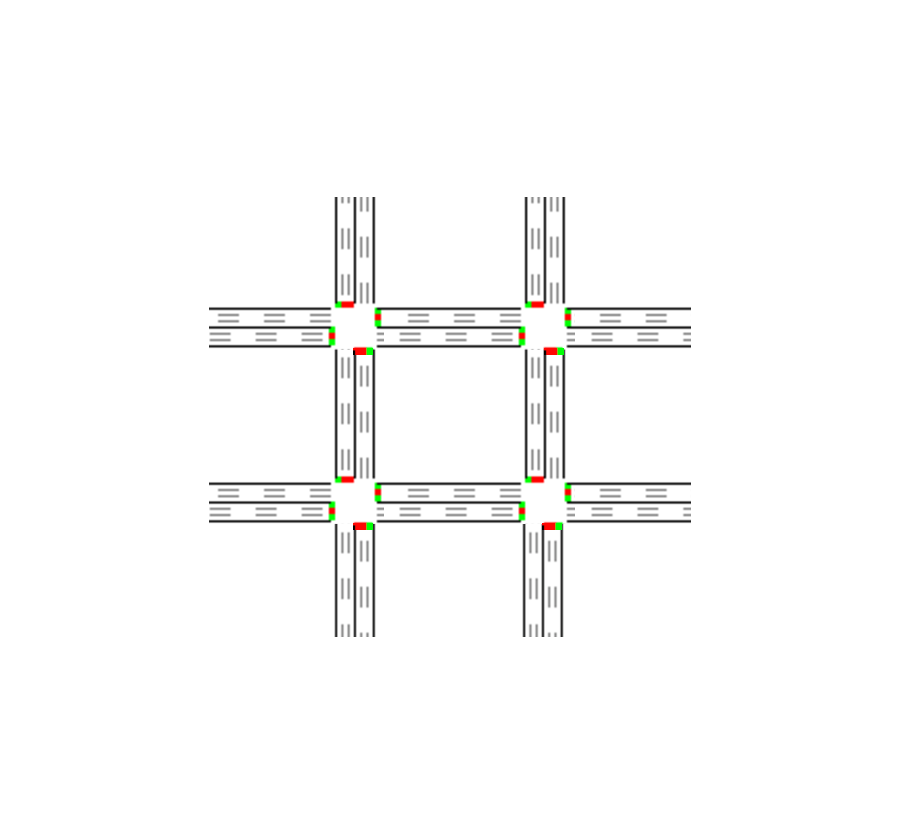
\includegraphics[width=0.25\textwidth]{figures/road_net_2_2.pdf} \vspace{-2mm}
% \caption{$2\times2$ road network.}\vspace{-2mm}
% \label{fig:net2}
% \end{figure}
% There are flat and peak (fluctuated) patterns for traffic flows and data are statistically synthesized from real-world traffic in Jinan and Hangzhou.
% \begin{itemize}
% 	\item Flat  \& Fluctuated
% 	% \item Undersaturated \& Oversaturated
% \end{itemize}
\item Real-world data. We use real traffic data in Manhattan, New York City. Detailed statistics are shown in Table~\ref{tab:real-table} and the road network of Manhattan is demonstrated in Figure~\ref{fig:road-net}. Note that the manhattan dataset contains signalized 2510 traffic lights.\\

\begin{figure}[t!]
  \centering
        % \begin{subfigure}[t]{.2\textwidth}
        %  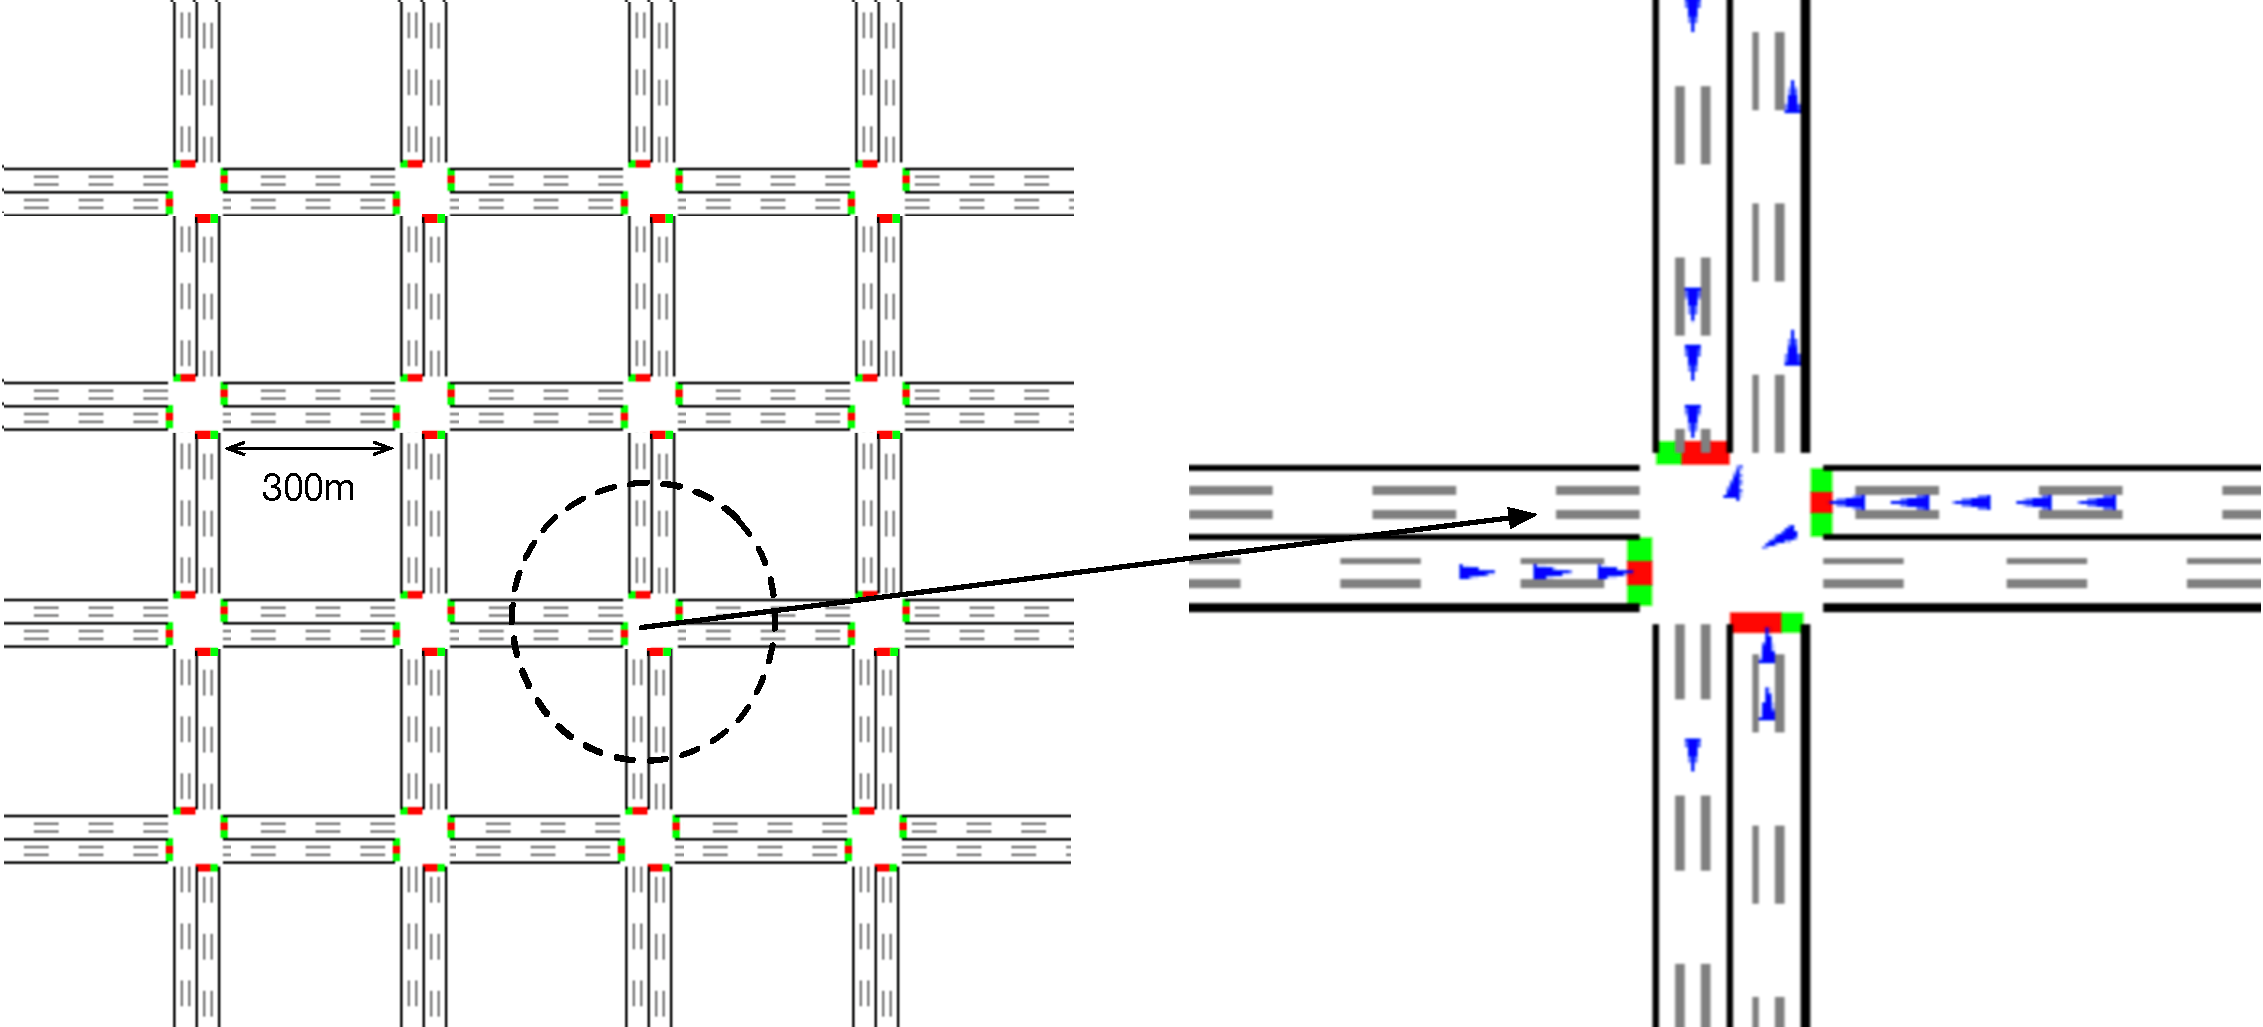
\includegraphics[width=\textwidth]{figures/road_net.pdf}
        %         \caption{$4\times4$ road network.}
        %         % \vspace{-.1in}
        %         \label{fig:manhattan}
        % \end{subfigure}
        % \hfill
        \begin{subfigure}[t]{.2\textwidth}
         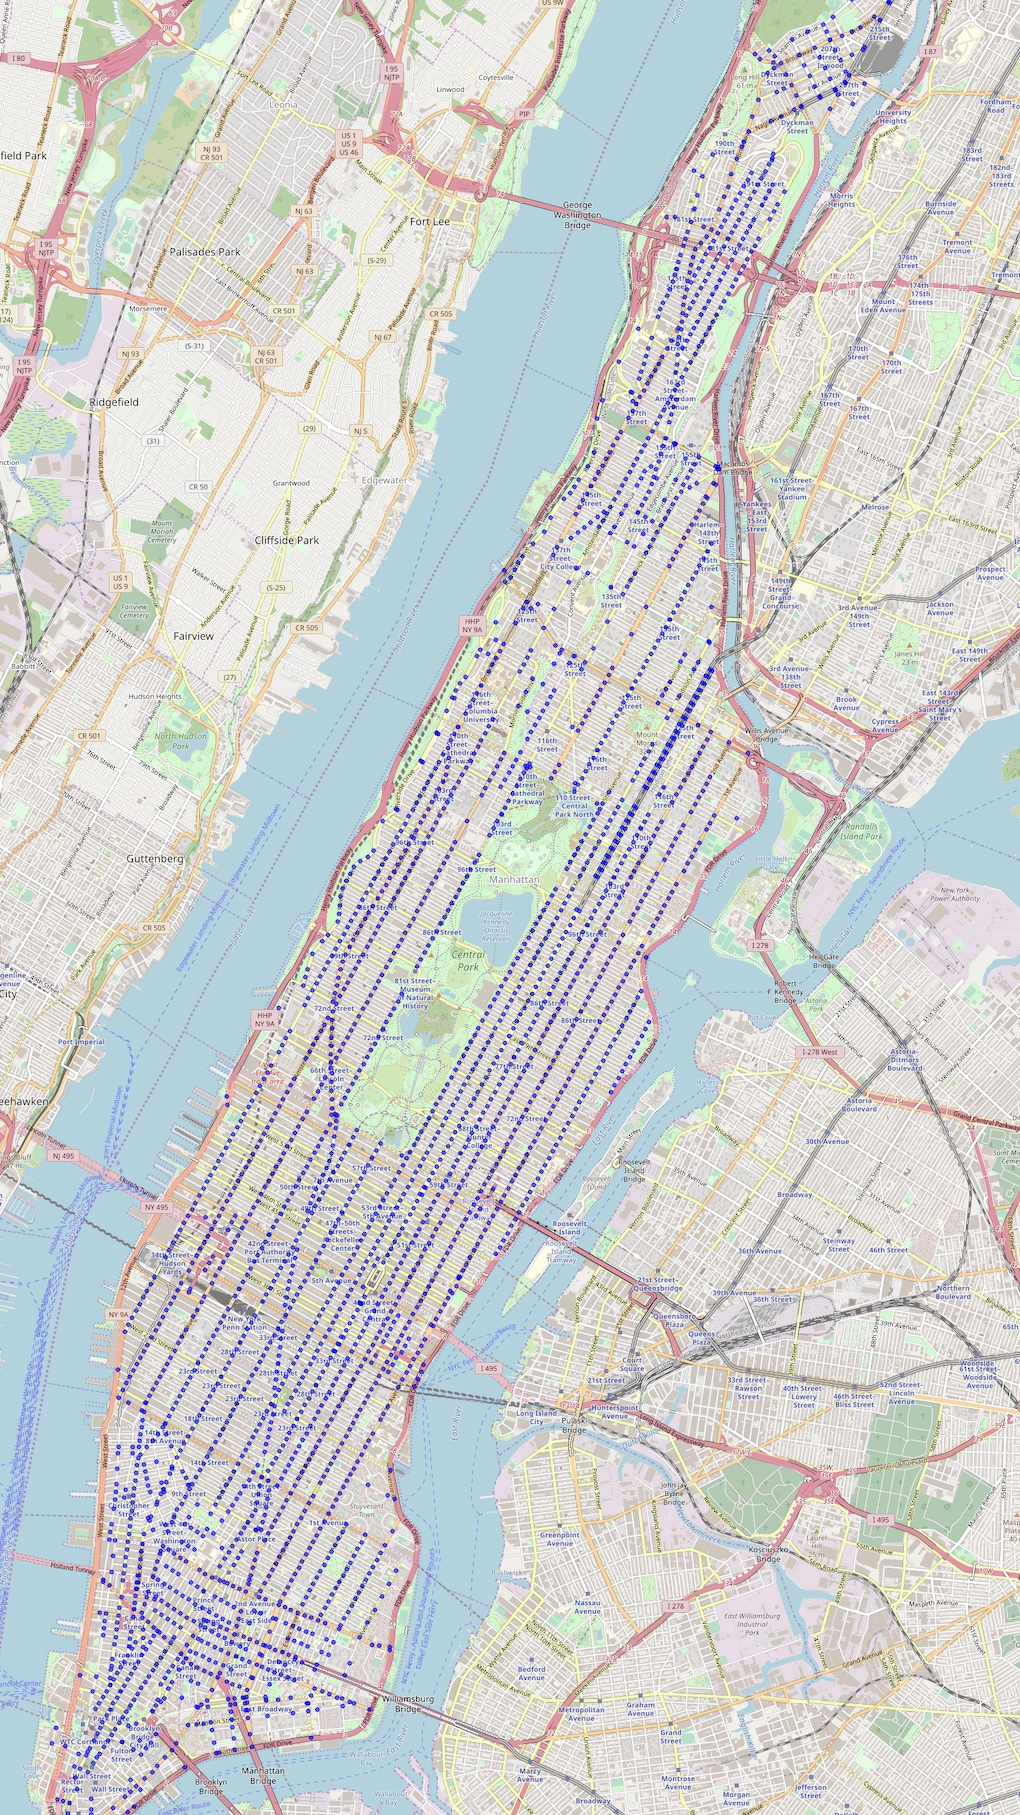
\includegraphics[width=\textwidth]{figures/IMG_2711.jpg}
                \caption{Manhattan}
                % \vspace{-.1in}

        \end{subfigure}
        \hfill
            \begin{subfigure}[t]{.2\textwidth}
         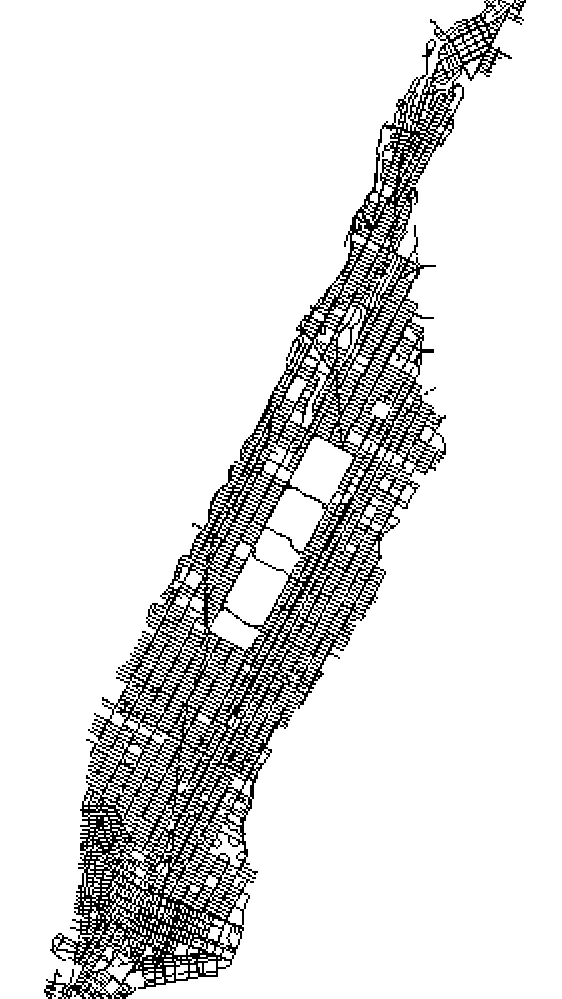
\includegraphics[width=\textwidth]{figures/IMG_2712.jpg}
                \caption{Manhattan in SUMO}
                % \vspace{-.1in}
        \end{subfigure}
        %         \begin{subfigure}[t]{0.45\textwidth}
        %  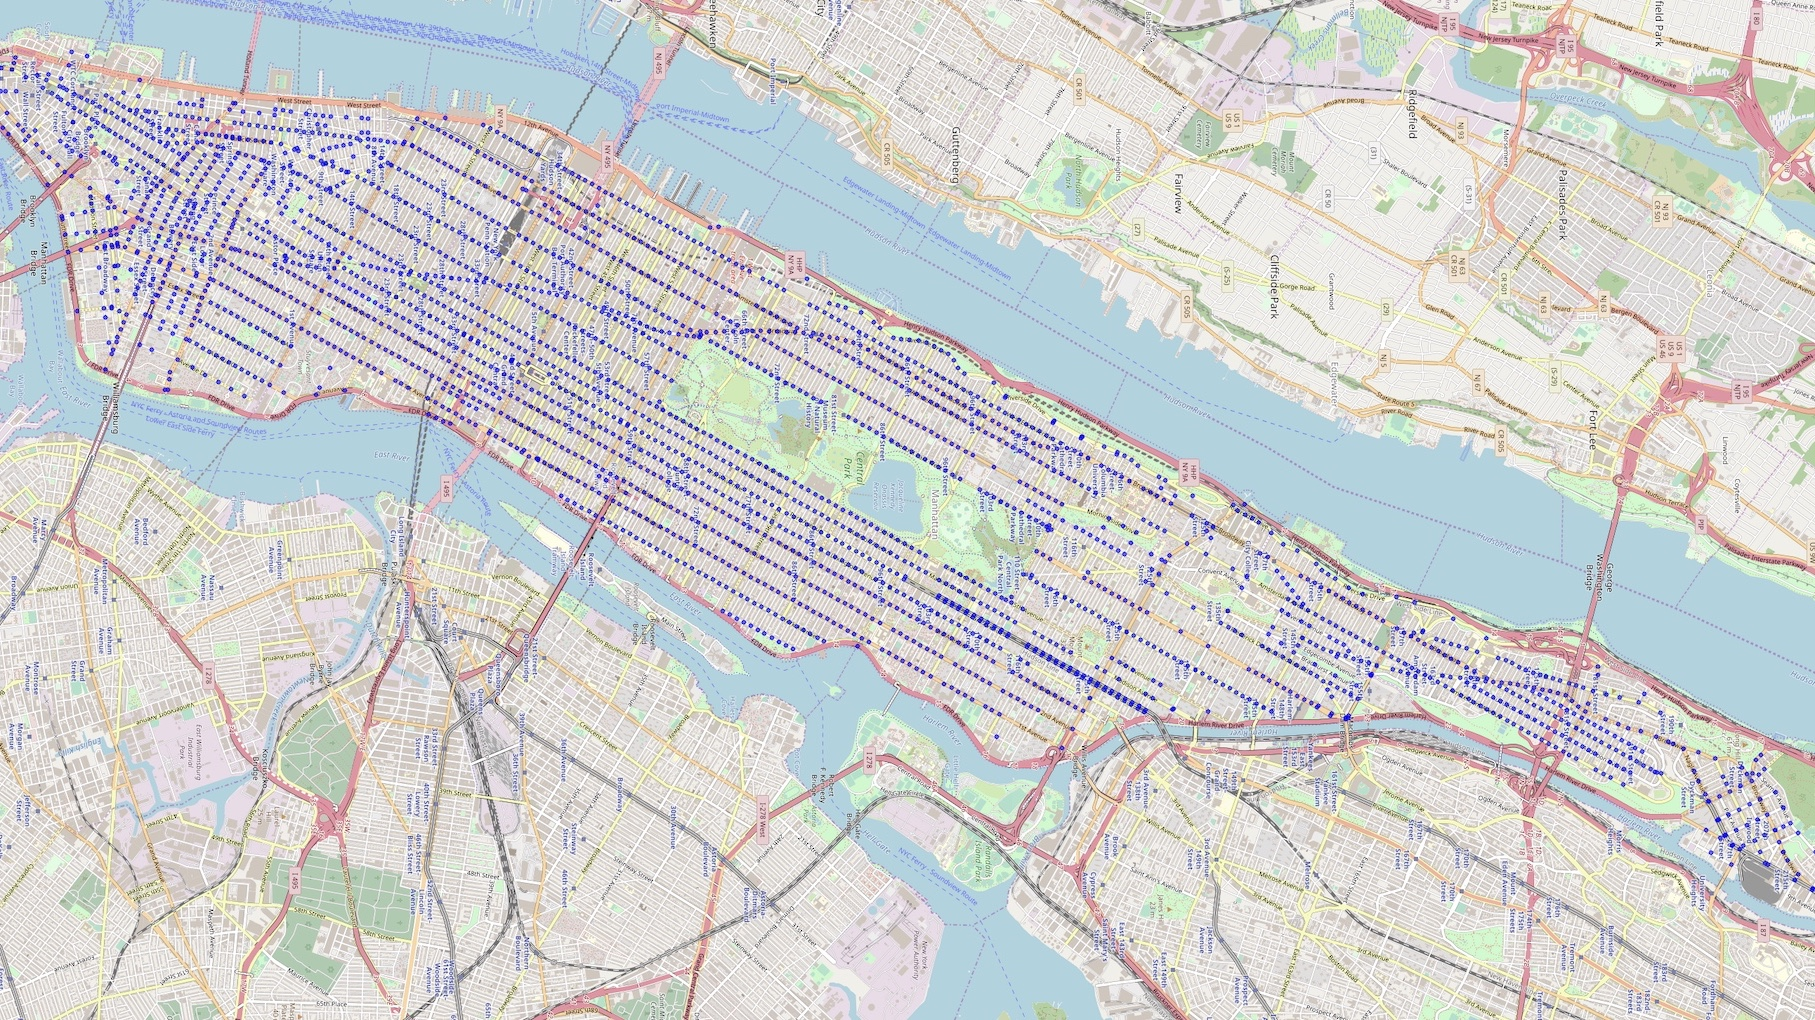
\includegraphics[width=\textwidth,height=0.13\textheight]{figures/manhattan-rotate.jpg}
        %         \caption{Manhattan}
        %         % \vspace{-.1in}

        % \end{subfigure}
        % \hfill
        %     \begin{subfigure}[t]{0.45\textwidth}
        %  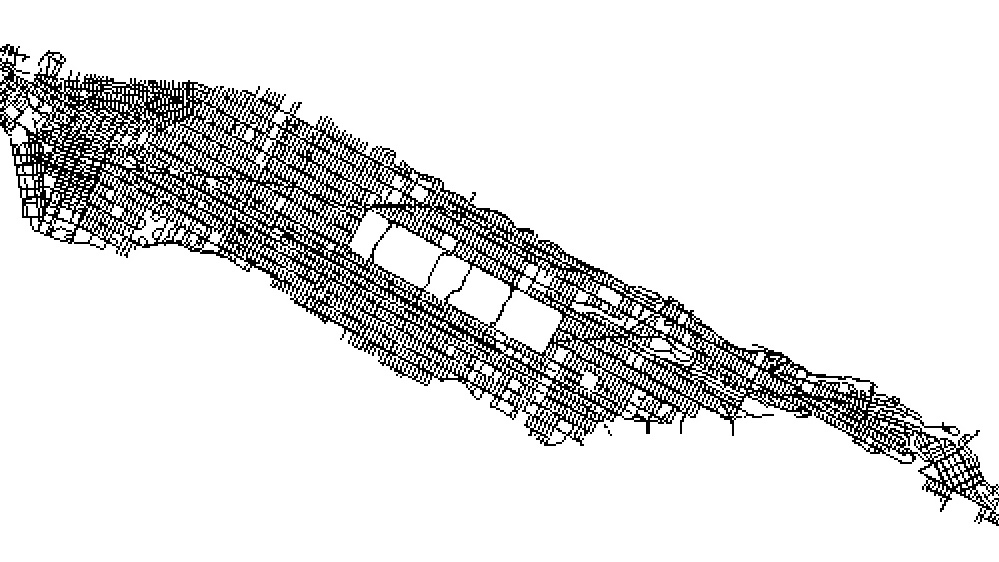
\includegraphics[width=\textwidth,height=0.13\textheight]{figures/manhattan-sumo-rotate.jpg}
        %         \caption{Manhattan in SUMO}
        %         % \vspace{-.1in}
        % \end{subfigure}
%   \subfigure[Config 1]{\label{fig:MFD_700_03} 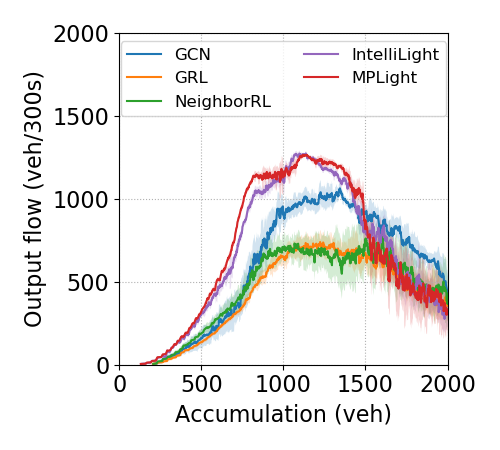
\includegraphics[width=0.3\textwidth]{figures/anon_4_4_700_03_synthetic.png}}
%   \subfigure[Config 2]{\label{fig:MFD_700_06} 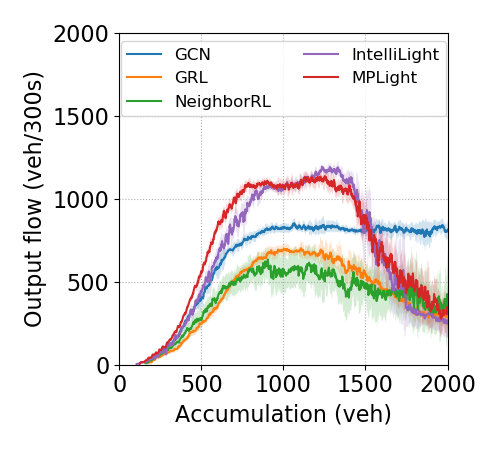
\includegraphics[width=0.3\textwidth]{figures/anon_4_4_700_06_synthetic.png}}
%   \subfigure[Config 3]{\label{fig:MFD_750_03} 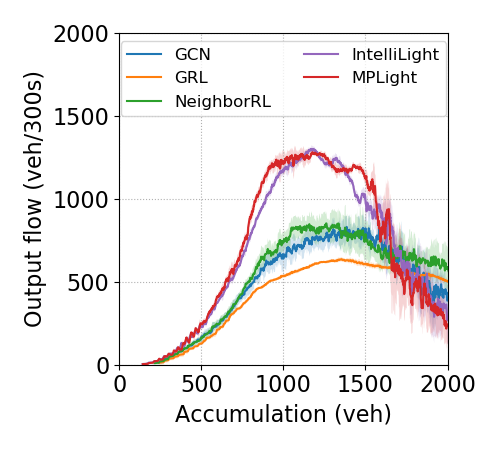
\includegraphics[width=0.3\textwidth]{figures/anon_4_4_750_03_synthetic.png}}
%   \subfigure[Config 4]{\label{fig:MFD_750_06} 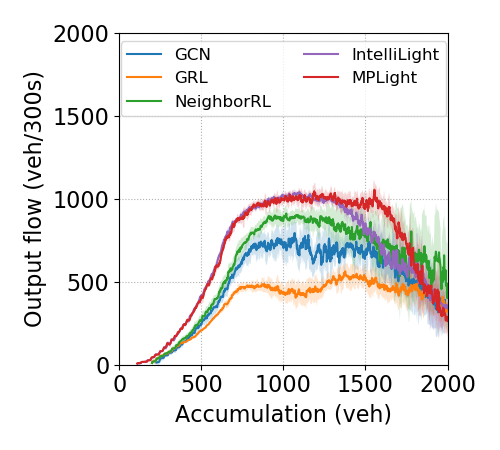
\includegraphics[width=0.3\textwidth]{figures/anon_4_4_750_06_synthetic.png}}
  \caption{Road network of Manhattan in our experiments.}
  \label{fig:road-net}
\end{figure}
% \todo{yuanhao}
% and make the manhattan figure beatiful
\end{itemize}
% \begin{figure*}[t!]
%   \begin{tabular}{cc}
%     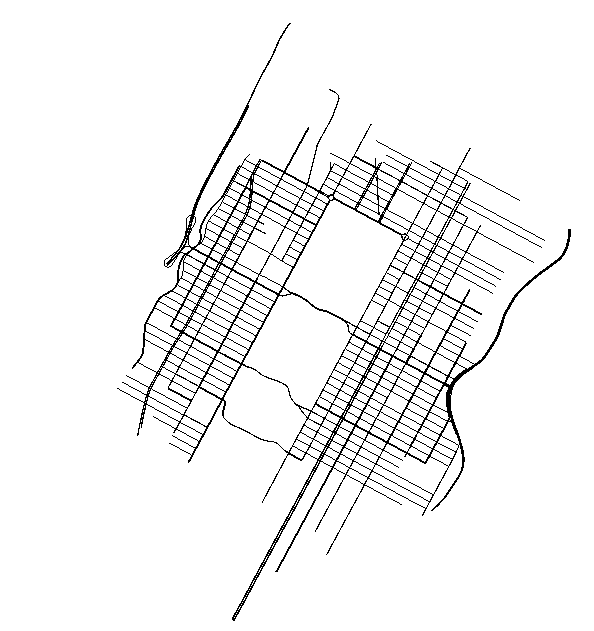
\includegraphics[width=0.5\textwidth,height=0.25\textheight]{figures/manhattan_1km.png} &
% \includegraphics[width=0.5\textwidth,height=0.25\textheight]{figures/manhattan_all.png} \\
% (a) manhattan\_1km & \multicolumn{1}{c}{(b) manhattan\_all} \\
%     \end{tabular}
% \\
% \caption{Manhattan}
% \end{figure*}

\begin{table}[h!]
\begin{center}
% \vspace{-3mm}
\caption{Four configurations of synthetic traffic data}
\label{tab:synthetic-table}
\begin{tabular}{ccc}
\toprule
Config        & \begin{tabular}[c]{@{}c@{}}Demand Pattern \end{tabular}  & \begin{tabular}[c]{@{}c@{}}Arrival rate (vehicles/s)\end{tabular}    \\ \midrule
1 & Flat           & \multirow{2}{*}{0.388}  \\\cmidrule(lr){1-2}
2 & Peak           &         \\ \midrule
3 & Flat           & \multirow{2}{*}{0.416}   \\\cmidrule(lr){1-2}
4 & Peak           &               \\ \midrule
\end{tabular}
% \\\footnotesize{$^{*}$ For illustrations about two patterns, see Figure~\ref{fig:Traffic-direc-pattern-1} and~\ref{fig:Traffic-direc-pattern-2} in Addendum.}\\
\vspace{-3mm}
\end{center}
\end{table}

% \todo{Weihua}

\begin{table}[t]
\caption{Data statistics of the real-world dataset}\label{tab:real-table}
\centering
% \hspace{-.3in} 
\begin{tabular}{cccccc}
\toprule
\multirow{2}{*}{Dataset}  & \multicolumn{4}{c}{Arrival rate (vehicles/h)}  & \multirow{2}{*}{\begin{tabular}[c]{@{}c@{}}\# of \\ Intersections\end{tabular}}\\
                           & Mean         & Std         & Max       & Min    &    \\\midrule
\begin{tabular}[c]{@{}c@{}} Manhattan \end{tabular} &   7576     &  586     &   4272     &  8220  & 2510    \\ 
\bottomrule
\end{tabular}

\end{table}


\subsubsection{Compared Methods}

\begin{itemize}
\item \FT~\cite{koonce2008traffic}: a policy gives a fixed cycle length with a predefined green ratio split among all the phases. It is widely used for steady traffic.
% \item \Greenwave~\cite{Roess2011t}: the optimal solution to control signals on the arterial with uni-directional small traffic flows. All the intersections share the same cycle length and the green ratio split, but with different offsets to form the green wave.
\item \Maxpressure~\cite{varaiya2013max}: the max pressure control selects the phase as green, in order to maximize the pressure according to the upstream and downstream queue length. It is the state-of-the-art control method in the transportation field for signal control in the network level.
\item \NIPS~\cite{van2016coordinated}: a deep Q-learning algorithm for coordinated traffic signal control. Specifically, the transfer planning and the max-plus coordination algorithm are employed for large-scale coordination.
\item \GCN~\cite{nishi2018traffic}: an RL-based traffic signal control method that employs a graph convolutional neural (GCN) network for representing geometric features among multiple intersections. 
\item \NeighborRL~\cite{arel2010reinforcement}: a multi-agent deep Q-learning algorithm that feeds the model with both its own and its neighbors' observations to implement network-level cooperation.
\item \Deeplight~\cite{wei2018intellilight}: the state-of-the-art deep Q-learning method to control signals in a single intersection. A phase selector and a memory palace are introduced for more efficient learning. 
% \item MARLIN~\cite{} 
\end{itemize}

\subsubsection[wide,noitemsep,topsep=0pt]{Evaluation Metrics}
We select the following two representative measures to evaluate different methods.
\begin{itemize}
\item \textbf{Travel time.} Average travel time of all vehicles spent in the system is the most frequently used measure to evaluate the performance of the signal control method in the transportation field.
\item \textbf{Throughput.} It is defined as the number of trips completed by vehicles and can reflect the effectiveness of the model combined with travel time.
\end{itemize}



\subsection{Performance Comparison (RQ1)}
In Table~\ref{tab:synthetic_performance}, we show the performance of transportation methods as well as Deep Reinforcement models on synthetic traffic data in Table. We can obviously discover that the proposed \PressLight consistently outperforms all the other methods in the four different scenarios, leading to both the least time cost of passengers and the maximum utilization of the road resource. The maximum reduction of travel time by \PressLight is $21.86\%$ over the second optimal solution \Maxpressure under Config 3, while the maximum enhancement of throughput over the second-best \Deeplight is as high as $13.07\%$ under Config 4.

The advantage of \PressLight over the other transportation and reinforcement learning methods can be attributed to its decent reward design and feedback learning from the environment at the same time. Compared with the other RL methods, \PressLight optimizes the control strategy by reducing the pressure between the entering and exiting lanes. Although the policy of \Maxpressure also depends on the pressure of different phases, there is a large performance margin from \PressLight in either travel time or throughput, since it ignores the assessment of previous action from the environment.

\begin{table*}[htbp]
\centering
\caption{Performance comparison of different methods evaluated in the four configurations of synthetic traffic data. For average travel time, the lower the better while for throughput, the higher the better.}
\label{tab:synthetic_performance}
\begin{tabular}{lcccccccc}
% {p{0.1\textwidth}p{0.07\textwidth}p{0.07\textwidth}p{0.07\textwidth}p{0.07\textwidth}|p{0.07\textwidth}p{0.07\textwidth}p{0.07\textwidth}p{0.07\textwidth}p{0.07\textwidth}}
\toprule
\multirow{2}[3]{*}{Model}&\multicolumn{4}{c}{Travel Time}&\multicolumn{4}{c}{Throughput}\\
\cmidrule(lr){2-5}\cmidrule(lr){6-9}
&Config 1&Config 2&Config 3&Config 4&Config 1&Config 2&Config 3&Config 4\\\midrule
\FT & 573.13 & 564.02 & 536.04 & 563.06 & 3555& 3477 & 3898 & 3556\\ 
\Maxpressure & 361.17 & 402.72 & 360.05 & 406.45 & 4702 & 4324 & 4814 & 4386\\ \midrule
\NIPS & 735.38 & 758.58 & 771.05 & 721.37 & 3122 & 2792& 2962 & 2991\\ 
\GCN & 516.65 & 523.79 & 646.24 & 585.91 & 4275 & 4151 & 3660 & 3695\\
\NeighborRL & 690.87 & 687.27 & 781.24 & 791.44 & 3504 & 3255 & 2863 & 2537\\
\Deeplight & 340.44 & 298.55 & 361.36 & 598.52 & 5097 & 5113 & 5483 & 4475 \\ \midrule
\textbf{\PressLight} & \textbf{309.33} & \textbf{262.50} & \textbf{281.34} & \textbf{353.13} & \textbf{5219} & \textbf{5213} & \textbf{5652} & \textbf{5060}   \\ 
% Improvements &   7.85\%          &  8.13\%           &       5.69\%         &      31.17\%       &   28.58\%          &    58.73\%             \\ 
\bottomrule
\end{tabular}
\end{table*}







% \begin{table}[]
% \begin{tabular}{|l|l|l|l|l|l|l|l|l|}
% \hline
%             & \multicolumn{4}{l|}{travel time}         & \multicolumn{4}{l|}{throughput}     \\ \hline
% config      & 1         & 2        & 3        & 4      & 1         & 2        & 3     & 4    \\ \hline
% FT          & 466.49    & 438.71   & 496.55   & 488.21 & 6924      & 6761     & 7465  & 7355 \\ \hline
% MP          & 353.29    & 450.65   & 516.00   & 531.53 & 7770      & 7704     & 8636  & 8428 \\ \hline
% IRL         & 348.13    & 400.30   & 322.40   & 391.89 & 2793      & 2829     & 4771  & 5045 \\ \hline
% MARLIN-ATSC &           &          &          &        &           &          &       &      \\ \hline
% PressLight  & 192.22    & 277.65   & 207.75   & 294.13 & 4588      & 4126     & 4960  & 5098 \\ \hline
%             & \multicolumn{4}{l|}{travel time}         & \multicolumn{4}{l|}{throughput}     \\ \hline
%             & Manhattan & Hangzhou & Jinan    & LA     & Manhattan & Hangzhou & Jinan & LA   \\ \hline
% FT          & 367.236   & 463.5019 & 428.856  &        & 1714      & 2524     & 5542  &      \\ \hline
% MP          & 486.81    & 386.047  & 410.8139 &        & 2223      & 2875     & 5801  &      \\ \hline
% IRL         &           &          &          &        &           &          &       &      \\ \hline
% MARLIN-ATSC &           &          &          &        &           &          &       &      \\ \hline
% PressLight  &           &          &          &        &           &          &       &      \\ \hline
% \end{tabular}
% \end{table}


% \subsection{Reward Function Study (RQ2)}
\begin{figure}[t!]
  \centering
        \begin{subfigure}[t]{.23\textwidth}
         \includegraphics[width=\textwidth]{figures/anon_4_4_700_03_synthetic.png}
                \caption{Config 1.}
                % \vspace{-.1in}
                \label{fig:MFD_700_03}
        \end{subfigure}
        \hfill
        \begin{subfigure}[t]{.23\textwidth}
         \includegraphics[width=\textwidth]{figures/anon_4_4_700_06_synthetic.png}
                \caption{Config 2.}
                % \vspace{-.1in}
                \label{fig:MFD_700_06}
        \end{subfigure}
        \hfill
        \begin{subfigure}[t]{.23\textwidth}
         \includegraphics[width=\textwidth]{figures/anon_4_4_750_03_synthetic.png}
                \caption{Config 3.}
                % \vspace{-.1in}
                \label{fig:MFD_750_03}
        \end{subfigure}
        \hfill
        \begin{subfigure}[t]{.23\textwidth}
         \includegraphics[width=\textwidth]{figures/anon_4_4_750_06_synthetic.png}
                \caption{Config 4.}
                % \vspace{-.1in}
                \label{fig:MFD_750_06}
        \end{subfigure}
  \caption{The macroscopic fundamental diagrams (MFD) of network traffic controlled by RL methods under four different configurations. It shows the relation between the total number of vehicles (accumulation) on the road and the rate at which trips reach their destinations (output flow). The higher the output flow, the better the signal control method.}
  \label{fig:MFD_analysis}
\end{figure}

\subsection{Road Resource Utilization Study (RQ2)}
In the transportation area, Macroscopic Fundamental Diagram (MFD) is used to reflect the relation between the vehicle accumulation in network and outflow of the network. As is shown in Figure~\ref{fig:MFD_analysis}, the horizontal axis is the total vehicle in the network, and the vertical axis is the total vehicles that complete their trips in the network. When the vehicle accumulation in the network is less than the sweet spot, the outflow of the network increases with the increase of the accumulation and then arrives at the
optimal throughput. If the vehicle accumulation is more than the sweet spot, the outflow decreases with the increase of the accumulation. Given the output flows of a network, a smaller accumulation indicates fewer vehicles in the network, indicating a better control strategy. Similarly, given the accumulations in a network, a higher output flow indicates the better control strategy. In Figure~\ref{fig:MFD_analysis},  \PressLight presents a higher output flow value given the same vehicle accumulation.

%Figure 4 plots the output flow and the network accumulation, it could be verified that the network present a fundamental diagram for different signal settings, i.e., the output flow at first increases as the accumulaiton grows, after a `sweet-spot', further accumulation will decrease the output. As we can see, that \PressLight is able to present a higher output flow value given the same vehicle accumulation and the `sweet-spot' of \PressLight is more upper left compared with other methods.

% Network infrastructure shows a property of MFD\\
% When demand conditions are steady, traffic flow streams on long homogeneous roads exhibit reproducible relations between their average flows and densities that engineers call “fundamental diagrams”. It has been recently proposed that entire city neighborhoods must also exhibit similar macroscopic fundamental diagrams (MFD) connecting the total number of cars on the road at any given time (the accumulation) with the rate at which trips reach their destinations (the output). It has also been proposed that the MFD of neighborhoods that are not too big should be independent of where people are going (the neighborhoods “origin-destination table”); i.e., the MFD should be a property only of the network infrastructure. Daganzo (2007) explains why.



% \subsection{Convergence Analysis}
\subsection{Impact of Parameter Sharing on Model Learning (RQ3)}
To investigate the impact of parameter sharing in model learning, we compare the performance of our RL agent design with and without parameter sharing under synthetic traffic. As is shown in Figure~\ref{fig:convergence}, parameter sharing enables our model to converge faster, which verifies the effectiveness of parameter sharing for controlling traffic signals.
% \begin{table}[htbp]
% \centering
% \caption{Number of episodes for different models to converge.}
% \label{tab:convergence}
% \begin{tabular}{ccccc}
% \toprule
% Model& config.1 & config.2 & config.3 & config.4 \\\midrule
% N model               & 19       & 30       & 93       & 112      \\\midrule
% One model             & \bf 7        & \bf 20       & \bf 77       & \bf 85\\\bottomrule      
% \end{tabular}
% \end{table}
% CONVERGE FIGURE{\color{red}todo-weihua}

\begin{figure}[htbp]
\centering
\includegraphics[width=0.5\textwidth]{figures/ccc_converge_ijcai.png}

\caption{Number of episodes for models to converge.}
\label{fig:convergence}
\end{figure}

% Figure 3 (number of trips ended as time)

% {\color{red} Can PressLight assure a network's vehicle accumulation remains as close as possible to the "sweet-spot" value?}

% No. But it is trying as best to maintain the sweet point value as long as possible if the traffic volume is increasing consistently, see (b).


% This result is promising for society because something simple and cheap (minimize delta q) can have a significant and verifiable benefit.

\subsection{Scalability Analysis (RQ4)}
In this part, we turn to experiments on real-world data. We evaluate our proposed method with other baselines under Manhattan, New York City, where there are over 2500 signalized intersections. The problem of such a large scale is usually difficult to deal with through conventional methods in the transportation field.

As shown in Table~\ref{tab:large-scale}, our method achieves the best performance over other baseline methods on both travel time and throughput. It should be noted that two methods including \NIPS and \NeighborRL can not be compared as they are unable to scale to large networks due to high complexity and computational costs. On the contrary, our proposed method \PressLight can handle traffic signal control for thousands of lights effectively and efficiently

% \begin{figure}[htbp]
% \centering
% \includegraphics[width=0.5\textwidth]{figures/manhattan_1km_real.png} \vspace{-2mm}
% \caption{manhattan 1km real}\vspace{-2mm}
% \label{fig:pressure}
% \end{figure}


% \begin{figure}[htbp]
% \centering
% \includegraphics[width=0.5\textwidth]{figures/manhattan_all_real.png} \vspace{-2mm}
% \caption{manhattan all real}\vspace{-2mm}
% \label{fig:pressure}
% \end{figure}




\begin{table}[htbp]
\caption{Performance of different methods on Manhattan.}
\begin{center}
\begin{tabular}{lcc}
\toprule
Model   & Travel Time&Throughput            \\\midrule
\FT         &  193.66        &     7398         \\
\Maxpressure&  133.72&              7620        \\\midrule
\NIPS       &   -$^{*}$        & -$^{*}$          \\
\GCN        &  139.01      &    5436            \\
\NeighborRL &  -$^{*}$       &     -$^{*}$           \\
\Deeplight  & 162.81   &   6816   \\\midrule
\PressLight &\bf 126.55&\bf8154\\\bottomrule   
\end{tabular}
\label{tab:large-scale}
\\
% \footnotesize{$^{*}$No result as **** can not scale up to thousands of intersections in New York's road network.}
\end{center}
No result as \NIPS and \NeighborRL can not scale up to thousands of intersections in New York's road network.
\end{table}



\section{Conclusion}

In this chapter, we propose a deep reinforcement learning method to tackle the problem of city-level traffic signal control. Specifically, we use theoretically guaranteed reward design and knowledge sharing to maximize the total throughput of the controlled region. We are the first to evaluate the RL-based traffic signal control methods in a real-world scenario with thousands of traffic lights. Our proposed method has shown its ability in delivering strong performance, generalization and its scalability.

We also acknowledge the limitations of our current approach and would like to point out a few possible future directions. First, we consider the scenario where only vehicles exist. However, in the real world, patterns of pedestrians and non-motorized vehicles, which can influence traffic signal control significantly, need to be taken into account. Second, although allocating a shared agent for all intersections achieves satisfactory control in the large-scale road network, more elaborate design for coordination and cooperation among neighboring intersections might further improve performance. Lastly, all experiments are currently carried out on a simulation platform. A field study would be an important future step for our model to get real-world feedback and for us to validate the proposed reinforcement learning approach.

  

% \input{tex/experiment}
% \input{tex/conclusion}
% \include
% \include{tex/example}
% \include{tex/faq}
% \include{tex/summary}

\appendix % 使用英文字母对附录编号

% 附录内容,本科学位论文可以用翻译的文献替代。
% \include{tex/app_setup}
% \include{tex/app_eq}
% \include{tex/app_cjk}
% \include{tex/app_log}

\backmatter % 文后无编号部分

% 参考资料
\printbibliography[heading=bibintoc]

% 致谢、发表论文、申请专利、参与项目、简历
% 用于盲审的论文需隐去致谢、发表论文、申请专利、参与的项目
\makeatletter

\ifsjtu@coursepaper
\else

  % "研究生学位论文送盲审印刷格式的统一要求"
  % http://www.gs.sjtu.edu.cn/inform/3/2015/20151120_123928_738.htm

  % 盲审删去删去致谢页
  \ifsjtu@review\relax\else
    %# -*- coding: utf-8-unix -*-
% !TEX program = xelatex
% !TEX root = ../thesis.tex
% !TEX encoding = UTF-8 Unicode
%TC:ignore
\begin{thanks}
I must express my very profound gratitude to my co-workers and advisors for providing me with unfailing support and continuous encouragement throughout my years of study and through the process of researching and writing this thesis.

\end{thanks}
%TC:endignore
         % 致谢
  \fi

  \ifsjtu@bachelor
    % 学士学位论文要求在最后有一个英文大摘要,单独编页码
    %# -*- coding: utf-8-unix -*-
% !TEX program = xelatex
% !TEX root = ../thesis.tex
% !TEX encoding = UTF-8 Unicode
\begin{bigabstract}


\end{bigabstract}
  \else
    % 盲审论文中,发表学术论文及参与科研情况等仅以第几作者注明即可,不要出现作者或他人姓名
    \ifsjtu@review\relax
      \include{tex/pubreview}
      \include{tex/projectsreview}
    \else
      \include{tex/pub}       % 发表论文
      \include{tex/projects}  % 参与的项目
      % \include{tex/patents}   % 申请专利
      \include{tex/resume}    % 个人简历
    \fi
  \fi
\fi

\makeatother

\end{document}
